\documentclass[letterpaper,12pt,onecolumn,final]{report}

\pdftrailerid{}
\pdfsuppressptexinfo15
\pdfminorversion=4

%% MANDATORY PACKAGES
\usepackage{cuthesis}         % Concordia's thesis style
\usepackage[english]{babel}   % load english localization
\usepackage{type1ec}          % type 1 font
\usepackage[T1]{fontenc}      % correct some font representation, needs cm-super fonts
\usepackage{times}            % use Times New Roman font
\usepackage[titletoc,title]{appendix}     % include Appendix command, add to ToC
\usepackage{setspace}         % control double/single line spacing
\usepackage[pdftex]{graphicx}
\usepackage{caption,tabularx,booktabs}
\usepackage{array}
\usepackage{csquotes}
\newcolumntype{C}[1]{>{\centering\arraybackslash}p{#1}}
%% OPTIONAL PACKAGES
%\counterwithout{footnote}{chapter}        % do no reset footnote # between chapters
\usepackage[hyphens]{url}     % print links
\usepackage{hyperref}         % provides hyperlinks (text different than link)
%\usepackage[hyphenbreaks]{breakurl}       % break long URL after hyphens
\hypersetup{
	colorlinks=true,
	breaklinks=true,
	linkcolor=black,
	citecolor=black,
	urlcolor=black,
	filecolor=black,
	linktoc=all,
}
\usepackage{graphicx}
%\graphicspath{{img/}}

\usepackage{blindtext}

%% CUSTOM MACROS
\usepackage{xspace}
\newcommand{\etal}{\textit{et al.}\xspace}
\newcommand{\etc}{\textit{etc.}\xspace}
\newcommand{\ie}{\textit{i.e.,}\xspace}
\newcommand{\eg}{\textit{e.g.,}\xspace}
\newcommand{\cf}{\textit{cf.}\xspace}
\newcommand{\supra}{\textit{Supra}\xspace}
\newcommand{\nee}{\textit{n\'ee}\xspace}
\newcommand{\aka}{\textit{a.k.a.,}\xspace}

% = = = Arrow -> (\lt)
\newcommand{\lt}{$\rightarrow$\xspace}

% = = = Keywords (kw)
\newcommand{\kw}[1]{\textsf{#1}}

% = = = Colored text (textblue)
\newcommand{\textblue}[1]{\textcolor{blue}{#1}}

% = = = Compact Lists (compactlist, compactlistn)
\newenvironment{compactlist}
  {\begin{itemize} 
  \setlength{\itemsep}{0pt} 
  \setlength{\parskip}{0pt}} 
  {\end{itemize}}
  
\newenvironment{compactlistn}
  {\begin{enumerate} 
  \setlength{\itemsep}{0pt} 
  \setlength{\parskip}{0pt}} 
  {\end{enumerate}}
  
\renewcommand{\labelitemi}{$\bullet$}
  

%------------------------Crypto----------------------%  

% = = = Zp, Gq and Zq
\newcommand{\Zp}{\mathbb{Z}^{*}_{p}}
\newcommand{\Zq}{\mathbb{Z}_{q}}
\newcommand{\Gq}{\mathbb{G}_{q}}

% = = = Encryption, etc.
\newcommand{\Enc}[1]{\mathsf{Enc}(#1)}
\newcommand{\EncB}[1]{\llbracket #1 \rrbracket}
\newcommand{\ReRand}[1]{\mathsf{ReRand}(#1)}
\newcommand{\Hash}[1]{\mathcal{H}(#1)}
\newcommand{\Sign}[1]{\mathsf{Sig}(#1)}
\newcommand{\Comm}[1]{\mathsf{Comm}(#1)}
\newcommand{\Open}[1]{\mathsf{Open}(#1)}

% = = = Tuples
\newcommand{\tuple}[1]{\left \langle #1 \right \rangle}


%-------------------Custom for Paper----------------------%

% = = = Name
\newcommand{\Name}{\textsf{System Name}\xspace}
\newcommand{\dai}{\textsf{Dai}\xspace}
\newcommand{\cdp}{\textsf{CDP}\xspace}
\newcommand{\vault}{\textsf{Vault}\xspace}

%\newcommand{\tickyes}{{\small\checkmark}}
%\newcommand{\tickno}{{\small$\times$}}
% TABLES:
\usepackage{adjustbox}
\newcommand{\headrow}[1]{\multicolumn{1}{c}{\adjustbox{angle=30,lap=\width-0.5em}{#1}}}
\newcommand{\full}{$\bullet$}
\newcommand{\prt}{$\circ$}
\newcommand{\none}{$\times$}
%% CUSTOM COMMANDS
%\newcommand{\subhead}[1]{\noindent{\textbf{#1.}}}
% !TEX root = ../main.tex

%------------------------LNCS----------------------%

%None

%------------------------Packages----------------------%

% = = = Graphics

\usepackage[table,xcdraw]{xcolor}

% = = = Subfig (note not subfigure)
\usepackage[caption=false,font=footnotesize]{subfig}

% = = = Math Symbols
\usepackage{amsmath}
%\usepackage{amstext,amssymb,amsthm}
\usepackage{bbm}
\usepackage{stmaryrd}
\usepackage{wasysym}
\usepackage{amssymb}
\usepackage{color}
\usepackage{multirow}
\usepackage{rotating}
\usepackage{makecell}
\usepackage{hhline}
% = = = Other
\usepackage{array}
\usepackage{color}
\usepackage[hyphens]{url}

%------------------------END----------------------%  
  


%% THESIS SETTINGS
\author{Mehdi Salehi}
\title{An Analysis of Upgradeability, Oracles, and Stablecoins in the Ethereum Blockchain}

% As of 2019, title is no longer used...
%\titleOfPhDAuthor{Mr.}         % or Ms., Mrs., Miss, etc. (only for PhD's)

% if PhD, uncomment:
%\PhD
% else if Master's, uncomment:
\mastersDegree{Master of Applied Science}

\program{Information and Systems Engineering}
%\program{Computer Science}
\dept{The Concordia Institute\\for\\Information Systems Engineering}
%\dept{The Department\\of\\Computer Science and Software Engineering}

%% See current GPD at https://www.concordia.ca/admissions/graduate/programs/contacts.html
\GpdOrChairOfDept{Dr.\ Mohammad Mannan}
\isGpd % Chair by default
%% See current Dean at  https://www.concordia.ca/ginacody/about/leadership/office-dean/dean-of-engineering-and-computer-science.html
\deanOfENCS{Dr.\ Mourad Debbabi} 
\chairOfCommittee{Dr.\ Amr Youssef}
\examinerFirst{Dr.\ Amr Youssef}
\examinerSecond{Dr.\ Ivan Pustogarov}
\supervisor{Dr. Jeremy Clark}
%% Following two lines are required if you have a co-supervisor
\hasCosupervisor
\coSupervisor{Dr. Mohammad Mannan}

%% Comment to use current month, needs to match initial submission
\submitmonth{April}
\submityear{2022}
%% Comment if date of defence is unknown yet, fill for final submission
\defencedate{April 1, 2022}


%%%%%%%%%%%%%%%%%%%%%%%%%%%%%%%%%%%%%%%%%%%%%%%%%%%%%%%%%%%%%%%%%%%%%%%%%%%%%%%

\doublespacing
\begin{document}

\begin{abstract}
{%trick to force double spacing in the abstract, otherwise some paragraphs may show single spaced
\setstretch{1.6667}

The Ethereum blockchain is a widely adopted global alternative to cloud computing platforms, currently used primarily for financial services. Given the large number of funds held by smart contracts and decentralized applications on top of Ethereum, there are profound security implications for both users and enterprise developers.

Over time, developers have brought more complex logic to Ethereum. For example, contracts often require access to valid, real-world data. In most cases, the system's functionality and security are strongly dependent on the correctness and safeness of the data pushed to the blockchain. One topic of this thesis is an oracle system---infrastructure added to the blockchain to respond to this need.
As contract code becomes more complex, it is increasingly likely that the code has bugs or vulnerabilities. Given smart contracts are immutable and tamper-proof, it seems impossible to upgrade a contract should a fix or patch be needed. Another topic of this thesis examines contract deployment patterns that enable and handle the upgradeability of smart contracts in Ethereum. Finally, the thesis also considers an application of oracle technology: payments made in stable currencies such as USD and not blockchain native currencies such as ETH, which are volatile in price. This thesis explains each topic in detail, evaluating the security risks of each, and examining any consequences for user trust and the degree of decentralization. 

% JC: try to keep to 1 page

%  broad adoption of decentralized applications brought another need in the service layers. The payments by user need to be This brings the idea of developing stablecoins pegged to a stable currency like the USD.

%Adding upgradeability patterns, oracles, and stablecoins to decentralized applications and smart contract logic adds significant security risks and the need to use a trusted third party, which is against disintermediation in the blockchain ecosystem. 
%  central trusted points that will be added because of each component. We also try to extend the design choices for each component to give the designer a broader spectrum, which may help make the systems more secure.

}
\end{abstract}

%\doublespacing
\begin{acknowledgments}
  I would like to thank my supervisors, Dr. Jeremy Clark and Dr. Mohammad Mannan, for their continued support and guidance during the course of my master's degree. Their constant support gave life to this project and made this thesis possible. I have learned a lot from them and would like to express my gratitude for their patience, motivation, and immense knowledge. I am fortunate to work under the close guidance of them, who inspired me with bright ideas, helpful comments, suggestions, and insights that have contributed to the improvement of this work.

  I would like to thank Shayan Eskandari, my colleague, for mentoring me during my master's and sharing his experience, and being by my side through this journey. I want to thank Mahsa Mousavi, my lab-mate, for her continuous feedback and support during our discussions and meetings. She has been very generous with her help during the course of my research.
  
  A very special word of thanks to my best friend in my life Nikoo Farvardin, who has always been a major source of support when things would get a bit discouraging. Her presence was significant in a process that is often felt as tremendously solitaire. She gave me support and help, discussed ideas, and prevented several wrong turns.
  
  In the end, I would like to acknowledge the unconditional affection and continuous support of my parents, my sister Neda, and my brother Saleh. They always fulfill all my silly demands and keep faith in my ability. They have always been the best inspiration in my life. I would like to dedicate this thesis to them. This journey would not have been possible without their encouragement and support. I am incredibly lucky to have them in my life.
\end{acknowledgments}


%%%%%%%%%%%%%%%%%%%%%%%%


%%%%%%%%%%%%%%%%%%%%%%%%


%%%%%%%%%%%%%%%%%%%%%%%%
\chapter{Introduction}


\section{Motivation}
Ethereum's native currency, ETH, is the second-largest cryptocurrency in the world in terms of total market capitalization at the time of writing this thesis. Bitcoin (BTC) is in first place but Bitcoin's protocol makes it difficult to deploy smart contracts as it only supports a limited scripting language. Thus, Ethereum is the most widely used blockchain that enables the deployment of verbose smart contracts with wide functionality. 

Smart contracts are pieces of code that run on blockchains such as Ethereum and eliminate the need of use of a trusted third party to run the logic. As Ethereum has its own native currency, users and smart contracts can make payments automatically including paying for the computation (gas fees).
Many projects are developing Decentralized Applications (Dapps) on Web3, which rely on smart contracts instead of traditional web applications (Web2) which rely on trusted, intermediary companies.
Also blockchains are immutable, which means that the transactions are irreversible under reasonable assumptions due to the nature of blockchain technology. 

Smart contracts can have control over large amounts of cryptocurrencies in their custody or in the custody of another smart contract. We have seen that vulnerabilities in code bases of smart contracts result in significant financial loss in DeFi and Ethereum and just in 2021, 1.3 billions of dollars are lost reported by Certik~\cite{certikReport}.

The technical and economical differences between Web2 apps and Web3 Dapps requires developers to adjust their mental model. This applies to the wave of new developers who have changed their careers to develop smart contracts on Ethereum in recent years, as well as professional experienced Web3 developers. The Ethereum blockchain may seem similar to a cloud service to some developers using it for the first time. But, there are nuances like immutable smart contracts that cannot be changed, and no access to real-world data or internet APIs that are off-chain. In this thesis, we try to shed light on some of the differences of Web3.


\section{Thesis Statement}
The primary aim of this dissertation is to shed light on specific problems Web3 developers face in Dapp development, including oracle systems, systems upgrades, and dealing with stablecoins. Over the course of time, developers tried to port more and more Web2 functionalities into Web3, but it almost always requires new risks or trusted third parties. Some of these risks and trust points are explored in this dissertation by answering questions below:

\begin{enumerate}
    \item \textbf{Question 1:} What methods exist for upgrading code on a blockchain that is supposed to be immutable, and which method is best when a new feature or a bug fix is needed?
    \item \textbf{Question 2:} What methods exist for granting smart contracts access to real-world data and APIs?
    \item \textbf{Question 3:} If a Dapp needs payment in a currency like USD, and not the native currency of the blockchain which is volatile, what methods exist for providing this and what are the risks?
\end{enumerate}


\section{Outline and Contributions}

The rest of this dissertation is organized as follows. In Chapter~\ref{ch:upgrade}, we summarize and evaluate six patterns, developed on Ethereum to enable upgradeability of smart contracts. Modern smart contracts use software tricks to enable upgradeability, raising the research questions of \textit{how} upgradeability is achieved and \textit{who} is authorized to make changes. We develop a measurement framework for finding how many upgradeable contracts are on Ethereum that use certain prominent upgrade patters. We also measure how they implement access control over their upgradeability: about 50\% are are controlled by a single Externally Owned Address (EOA), and about 13\% are controlled by multi-signature wallets in which a limited number of persons can change the whole logic of the contract which is a risk to the Ethereum ecosystem.

In Chapter~\ref{ch:oracle} we describe that one fundamental limitation of blockchain-based smart contracts: contracts execute in a closed environment and only have access to data and functionality that is already on the blockchain, or that is fed into the blockchain. Any interactions with the real world need to be mediated by a bridge service, which is called an oracle. As decentralized applications mature, oracles are playing an increasingly prominent role. With their evolution comes more attacks, necessitating greater attention to their trust model. We dissect the design alternatives for oracles, showcase attacks, and discuss attack mitigation strategies.

In Chapter~\ref{ch:dai} we shed light on a number of Ethereum projects for stablecoins and synthetic assets use the same core mechanism for fixing the price of an asset. In this chapter, we distil this shared approach into a primitive we call red-black coins. We use a model to demonstrate the primitive's financial characteristics and to reason about how it should be priced. Real world projects do not use the red-black coin primitive in isolation but lay on other mechanisms and features to provide fungibility and to reduce exposure to price drops. One mechanism is called liquidation, however liquidation is hard to analyze as it relies on human behavior and could produce unintended economic consequences. Therefore we additionally develop a design landscape for extending the red-black coin primitives and put forward a research agenda for alternatives to liquidation.

In Chapter ~\ref{chap:conclusion} we provide some concluding remarks and future research directions.



%\paragraph{Academic Paper. }The work on oracles discussed in this dissertation in Chapter~\ref{ch:oracle} has been peer-reviewed and published in the following article:
%
%\begin{displayquote}
%Eskandari, Shayan, et al. "Sok: Oracles from the ground truth to market manipulation." Proceedings of the 3rd ACM Conference on Advances in Financial Technologies. 2021.
%\end{displayquote}
%
%\paragraph{Academic Paper. }The work on stablecoins discussed in this dissertation in Chapter~\ref{ch:dai} has been peer-reviewed and published in the following article:
%
%\begin{displayquote}
%Salehi, Mehdi, Jeremy Clark, and Mohammad Mannan. "Red-Black Coins: Dai without liquidations." International Conference on Financial Cryptography and Data Security. Springer, Berlin, Heidelberg, 2021
%\end{displayquote}
\chapter{Background}
\label{chap:background}
This chapter covers background information discussed in this dissertation. 

\section{Ethereum Basics}

Ethereum is a state machine that is globally accessible and its Ethereum Virtual Machine, applies the changes to the state based on the rules defined for the Ethereum network. Ethereum is often described as ``world computer'' because anybody from anywhere can have access to the Ethereum and use the stack of Ethereum and the EVM to execute their computations. 

Ethereum is the next generation of blockchains compared to Bitcoin. Bitcoin is just handling payments and some specific limited logic based on a limited scripting language which is called ``Bitcoin Scripting Language''. For instance, bitcoin scripts cannot handle loops. But in Ethereum, EVM can handle more general and complex codes named \textit{Smart Contracts}. EVM is quasi-Turing-complete state machine. It is ``quasi'' because computation in Ethereum is bounded to specific number of gas; unit of measurement of computations and storage resources in Ethereum. 

Users can work with Ethereum blockchain by sending transactions to the network. They can just transfer Ether (or ETH), the native currency of Ethereum blockchain, or they can do their desired computations by execute smart contract functionalities in Ethereum. Users must pay the fee to work with Ethereum. This fee is calculated paid in gas, and it is based on the amount of computations and storage load on the Ethereum network and also network congestion.  

For more details about the basics of Ethereum, we refer chapter one and two of~\cite{antonopoulos2018mastering} to the readers eager to learn more about Ethereum.
In the further sections, we explain the more detailed aspects of Ethereum Virtual Machine (EVM), Ethereum infrastructure, and Decentralized Applications (Dapps) running on top of Ethereum. 

\section{Dig Deeper into Ethereum}
Smart contracts are pieces of codes that are deployed to a blockchain systems, to remove the barrier of trusting middleman and to run specific logic. Ethereum is the first and mostly used public blockchain that introduced rich smart contracts that are not just limited to some specific scripts (like Bitcoin scripting language). Smart contracts are supposed to be immutable and tamper proof which means the code cannot be changed just after deployment to the blockchain.

Smart contracts (in Ethereum) are usually written in High-Level programming languages such as Solidity and Vyper and compiled into a Low-Level EVM bytecodes using a compiler (\eg Solc). An EVM bytecode is a binary string that is interpretable by EVM. Then EVM bytecode will be deployed to the Ethereum main blockchain.

To understand the process of deployment of a smart contract one should have familiarity with different types of accounts in Ethereum. There are two types of Ethereum accounts: \textit{Externally Owned Account (EOA)} and \textit{Contract Account}. 
EOA is an account that is controlled by a private key and keeps balance of Ethers that the account has and also a \textit{nonce}, which indicates the number of transactions sent by the account and act like a counter to mitigate replay attacks. Any external actor can generate a random private key and use ECDSA encryption algorithm to generate the public key from the private key. Ethereum uses SECP-256k1 curve for ECDSA as described in the Ethereum yellow paper.
The EOA addresses can create new transactions, sign them with the private key related to the account and send it to Ethereum network to be confirmed and recorded on the main Ethereum chain. This transaction can:
\begin{enumerate}
    \item Send Ether to another EOA.
    \item Create a new \textit{Contract Account} by sending a bytecode.
    \item Calling a \textit{Contract Account} to execute a logic.
\end{enumerate}

Each transaction type is explained below:

\paragraph{Sending Ether.} 
For sending Ether into another EOA account the sender should specify the address which should be an EOA and not a contract account and also an amount to be sent.

\paragraph{Creating a new Contract Account.}
Creating a new \textit{Contract Account} is a bit tricky. The EOA should send a transaction containing the bytecode of the contract and setting the destination address to \emph{null}. Then EVM will create an address for the newly generated contract. The newly generated account (which is a contract account) keeps four fields: A \textit{nonce} which is similar to nonce in EOA and keeps track of number of transactions created by that account, Ether balance which indicates number of Ether the account holds, \textit{Contract Code} which keeps the bytecode of the account which is executed each time a transaction calls the account, and \textit{Contract Storage} which is a Merkle Patricia Tree data structure that maintain the data related to the contract account. Detailed explanation of the contract storage can be found in Section~\ref{sec:storagelayout}. 
The other important aspect of contract creation in Ethereum is how EVM generate the address for newly generated contract account. In EOA contract creation, EVM calculates the contract address by using the transaction sender's address and it's nonce. The formula is show below:
\begin{equation}
    \label{eqn:create}
    Address = keccak256(rlp.encode(Sender Address, nonce))[12:]
\end{equation}
In this formula \textit{keccak256} is the \textit{sha3} hash used in Ethereum blockchain. Also \textit{RLP} (Recursive Length Prefix) encoding is used in Ethereum to encode arbitrary nested arrays of binary data, such as transactions data. Also at the end, EVM picks the last 20 bytes of the hash as the result address.

In addition, contract accounts also can create a new contract account using two different EVM opcodes: \texttt{Create} and \texttt{Create2}. For transactions originated by a contract account and consist of these two opcodes, EVM will deterministically calculate the address for the new account and then create a contract account with the related four fields explained above. The whole process of contract creation is similar for these two opcodes, but the main difference is how EVM calculates the address for the contract account. For \texttt{Create} opcode the calculation formula is the same as formula EVM uses for EOA contract creation (Formula~\ref{eqn:create}).\footnote{Here the nonce is the nonce of contract account.} But, for \texttt{Create2} opcode, EVM uses completely different formula to calculate it. In this type, EVM calculates the address by using sender's address and bytecode that is sent to be deployed (a.k.a init code). Because the formula does not contain nonce and all other variables are predictable, the newly generated address in this type is \emph{Predictable}. The formula for contract address calculations using \texttt{Create2} is:

\begin{equation}
    \label{eqn:create2}
    Address = keccak256(0xff + senderAddress + salt + keccak256(init-code))[12:]    
\end{equation}

Based on the formula~\ref{eqn:create2}, if the same sender address, tries to deploy the same initialization code, the address will be the same. But, EVM does not permit to redeploy a contract if there is still a contract account related to that address. But, there is a way to delete the previous contract account and then re-deploy the contract on the same address. If the contract contains \texttt{SELFDESTRUCT} opcode, by calling it the whole contract account along with it's four field will be wiped out and so there is a chance to re-deploy the contract. The whole process is explained in detail in Chapter~\ref{ch:upgrade}. 

\paragraph{Calling a \textit{Contract Account} to execute a logic.}
The last way of interaction of an EOA with Ethereum is sending a transactions by which calling a contract code to execute its logic. If the recipient (destination) of the transaction is a contract account, EVM will start executing its contract code automatically. To explain it better we split the process into two steps describe below:

\paragraph{Transaction Creation by user. }Suppose contract A has function ``setNumber'' to set a \textit{uint}\footnote{Unsigned Integer} variable ``num'', that takes the new amount as input. If Alice decides to set a new number, for instance 3, to the num variable, she should send a transaction specify the recipient as contract A's address. Also transactions to a contract have another field named ``data'' in which the user indicates which function of the contract is going to be called and what are the inputs for the function call. The data part of the transaction is also known as ``Call-Data'' field. Alice should declare that she is going to call ``setNumber'' function with input 3. Defining the target function in EVM is not by putting the name of function. 

EVM uses \textit{Function Selector} to recognize the functions which is the first four bytes of the Keccak-256 hash of the \textit{function signature}. The function signature is defined as the function name with the list of parameter types divided by a comma - no spaces are used. For instance, for our case the function signature is ``setNumber(uint)''. So, Alice calculates the function signature using this formula:

\begin{equation}
    Function Selector = Bytes4(keccak256("setNumber(uint)")) = 0x234a4ac2
\end{equation}

Now Alice has the function selector and can generate the call data of the transaction by putting together the function selector and the encoded inputs in the defined order. The transaction is created and should be signed by Alice and send to the Ethereum network.

\paragraph{Execution Process. } 
The next step is to describe how EVM interpret and execute the transaction sent by Alice. EVM checks the recipient of the transaction and because it is the address of contract A, it will start executing the bytecode of contract A. Bytecodes in Ethereum first extract the first four bytes of call data of the transaction. Then checks that if the function selectors in the bytecode is match with the first four bytes of the call data. If a function selector found, it means that the user called that specific function of the contract (in our case, setNumber function of contract A). If EVM cannot find any function selector that matches the first four bytes of call data, then a function named \textbf{Fallback} function will be called. The Fallback function is a function defined in the high level languages (\eg Solidity) and supposed to be executed if EVM could not find function selector equal to the first four bytes of calldata or also if the calldata is empty (\ie sending Ether to the contract without function call). 

In each function, in the bytecode, first EVM will extract the inputs related to the function from calldata and then execute the logic of that function with the provided inputs.

Also it should be mentioned that a contract can also call a function of another contract providing the related function selector and inputs and the other processes are the same. This type of call are called \textbf{Internal Calls}. In literature it is also called \textbf{Messages} instead of transactions and will be discussed in detail in Section~\ref{sec:txVsMsg}.

There are other technical explanations needed about Ethereum that a reader should know for this dissertation which we will describe below:

\subsection{Run-time Bytecode vs. Contract Creation Code}
%run time and contract creation
In Ethereum the code that is sent to create contract (a.k.a \textbf{Contract Creation Code}), may be different with the code that is stored in the blockchain for that contract account (a.k.a \textbf{Run-time bytecode}). Run-time bytecode is the bytecode which is saved in the blockchain as the code of that specific contract account and each time the contract is called, this code will be executed by EVM. But, Contract Creation code is the input data of the transaction by which a user or a contract tries to deploy a new contract. The Contract Creation code has a field, named \textit{init code}, which is responsible to: 1) make changes to the state of the contract (initializing the storage variables using a constructor), 2) put the run-time bytecode to the memory 3) put the length of the run-time bytecode in the memory 4) put the offset in the memory where the run-time bytecode is saved in the stack 5) execute the \texttt{Return} opcode to push EVM to deploy the contract.\footnote{\url{https://leftasexercise.com/2021/09/05/a-deep-dive-into-solidity-contract-creation-and-the-init-code/}} 

So, the run-time bytecode could be completely different from the contract creation code. It will be discussed in the detail in Chapter~\ref{ch:upgrade} in Section~\ref{sec:metamorphic}.

\subsection{Storage Layout in EVM} \label{sec:storagelayout}
In Ethereum each contract account holds state in its own permanent storage. EVM uses an uncommon storage structure to store the storage state based on the variable types. It uses 32-bytes to 32-bytes key-value mapping to store the data which are zero initialized. Except dynamic arrays and mappings, the other variable types are stored in this structure contiguously one after another starting from slot 0. 

Mappings and dynamic arrays cannot be saved contiguously, because their size is unpredictable. So for dynamic arrays if the storage location after applying the rules ends up at slot P, the size of the array will be saved in this slot and the elements of the array will be saved contiguously starting from slot \textit{keccak256(p)}.

For mapping instead of dynamic array, zero will be saved in slot P. Also element of the mapping with key equal to K is stored in slot \textit{keccak256(h(K), p)} where h is keccak256 of the key value padded to 32 bytes~\cite{wood2014ethereum}.

The storage variables are accessible on-chain if there is a getter function inside the contract that gives the variable amount. Marking a variable as public is also give the opportunity to read the data on-chain because Solidity compiler creates a getter function for all public variables. 

To read the data off-chain, one need to have access to an Ethereum node which is discussed in Section~\ref{sec:nodes}.


\subsection{Transaction vs. Message}\label{sec:txVsMsg}
We discussed Ethereum transactions in detail in the previous sections. A message is very similar to a transaction but it is produced by another contract instead of an EOA. Messages are the way that contracts calling each others' functions. A message is produces when a contract uses a \texttt{CALL}, \texttt{DELEGATECALL} or \texttt{STATICCALL} opcodes. So, a function from another contract will be executed. The main difference between \texttt{CALL} and \texttt{DELEGATECALL} opcodes is that by \texttt{CALL}ing another contract the storage layout of the the destination contract will be changed. But, \texttt{DELEGATECALL}ing another contract, keeps the contract context. It means that the storage layout of the caller contract will be changed instead of the destintion contract. It is analogues to copy pasting that specific function in the caller contract and running its logic inside the caller contract. There are risks regarding \texttt{DELEGATECALL} opcode and the fact that it keeps context such as \textit{function selector clashes} and \textit{storage layout clashes} which will be discussed in more details in Chapter~\ref{ch:upgrade}, Section~\ref{sec:delegatecall}.

Also it worths mentioning that \texttt{STATICCALL} act completely similar to \texttt{CALL} opcode, except it will be reverted if the message tries to change the state during the call. 
\footnote{\url{https://ethdocs.org/en/latest/contracts-and-transactions/account-types-gas-and-transactions.html}}


%compiler ??!!

\subsection{Off-chain Access to the Blockchain Data}\label{sec:nodes}

To have access to the data stored in Ethereum blockchain, one should have access to an ``Ethereum Node''. Ethereum node refer to running a piece of software called Ethereum client, which implemented the rules and specifications defined by Ethereum yellow paper~\cite{wood2014ethereum} to join and sync with Ethereum network and to keep Ethereum network and data secure and safe.
\footnote{\url{https://ethereum.org/en/developers/docs/nodes-and-clients/}} 

There exists various implementations for Ethereum client in different languages (\eg Go, Rust, JavaScript,\etc). ``Geth'' is the most widely used Ethereum client written in Go. 
There are three different types of Ethereum nodes: Light node, Fast-sync and Archive full node.

\textit{Light node} stores the headers of the blocks and can have a limited verification such as state root verification. This type of clients are useful for devices that cannot store huge data.
\textit{Fast-sync Full node} stores all blockchain data, and can participate in new block generation. Also all past states can be derived from the full node but it takes time to grab the past data.
\textit{Archival Full node} not only stores all blockchain data, but also index them as well so that historical states can be accessed quickly on demand. In this thesis we call Archival Full node a
full node. 

An Ethereum full node has a JSON-RPC API that gives the user chance to use the methods implemented by the client and read the Ethereum data off-chain. Some of the methods that are used in this paper is listed below:

\begin{itemize}
    \item \emph{trace\_block}: Returns the transaction traces of all transactions in a specific block.
    \item \emph{eth\_getStorageAt}: Returns the value stored in a specific slot of a determined address. 
    \item \emph{eth\_getCode}: Returns the bytecode stored for the specific account address. If the address is EOA, it will return 0x0.
\end{itemize}

\section{Ethereum Use-cases}

In the previous section we mostly discussed the infrastructure of Ethereum and give the details about how Ethereum works under the hood and also how users can work with it. 
This section is mostly talk about the use-cases and nuances regarding them in Ethereum. Before explaining the use-cases one by one, we should shed light into one of the main obstacles that blockchain systems such as Ethereum has for developing different applications.


\paragraph{The Oracle Problem.}  

Smart contracts cannot access external resources (\eg a website or an online database) to fetch data that resides outside of the blockchain (\eg a price quote of an asset). External data needs to be relayed to smart contracts with an oracle. An \emph{oracle} is a bridge or gateway that connects the off-chain real world knowledge and the on-chain blockchain network. The `oracle problem'~\cite{linkOracleProblem} describes the limitation with which the types of applications that can execute solely within a fully decentralized, adversarial environment like Ethereum. Generally speaking, a public blockchain environment is chosen to avoid dependencies on a single (or a small set) of trusted parties. One of the first oracle implementations used a smart contract in the form of a database (\ie mapping\footnote{A Solidity \texttt{mapping} is simply a key-value database stored on a smart contract.}) and was updated by a trusted entity known as the \texttt{owner}. More modern oracle updating methods use consensus protocol with multiple data feeds or polling techniques based on the ``wisdom of the crowd''. The data reported by an oracle will always introduce a time lag from the data source and more complex polling methods generally imply longer latency.

\paragraph{Trusted Third Parties.} A natural question for smart contract developers to ask is: if you trust the oracle, why not just have it compute everything? There are a few answers to this question: (1) there may be benefits to minimizing the trust (\ie to just providing data instead of full execution), (2) there are widely trusted organizations and institutes---convincing one to operate an oracle service is a much lower technical ask than convincing one to operate a complete platform, and (3) if a data source becomes untrustworthy, it may require less effort to switch oracles than to redeploy the system. 

To mitigate the problem stated above, different solutions are developed to answer the oracle problem and provide data for the applications in Ethereum that needs the real-world data. We will discuss the problem and solution in detail in Chapter~\ref{ch:oracle}.

There are myriad of applications developed on top of Ethereum blockchain. Some of them uses the solutions describe in  Chapter~\ref{ch:oracle}, using one of them to address the oracle problem and bring real-world data on-chain. In later part of this section, we will explain the most favorable use-cases and applications on Ethereum.

\subsection{Stablecoins/Synthetic Assets}

A ``synthetic asset'' is an asset that tracks the price of another asset without holding the obligations of that asset. For instance, a synthetic asset of Apple share tracks the price of Apple share that does not receive dividends and not have any other obligations regarding the Apple share. This can be done by having the price of the asset provided by an oracle which is discussed above and some other ad-hoc mechanisms to stabilize the price of the asset that will be explained in Chapter~\ref{ch:dai}. An example Dapp that is providing synthetic assets is \textit{Synthetix}\footnote{\url{https://synthetix.io}}.

The asset can also be a currency (\eg USD) and in this case, it will be a stablecoin. A stablecoin is an asset that supposed to be peg to a currency such as USD. There are a myriad of stablecoin platform in Ethereum such as \dai which we will discuss in Chapter~\ref{ch:dai}

\subsection{Decentralized Exchange (DeX)}
Decentralized Exchanges (DeX) are platforms that helps users to exchange their assets without need of an intermediary. Two main types of Decentralized Exchanges are Automated Market Maker (AMM) and orderbook-based exchanges. 

In AMMs a party named Liquidity Provider (LP), creates pools for pairs of assets (could be more than two assets in a pool like Balancer protocol), and put liquidity on the pool. Users can exchange their assets in the pool. The smart contract will calculate the amount a user receive for a trade, using a mathematic formula based on the amount of liquidity in the pool and the amount user wants to exchange. Because the calculations and market making is done by smart contract automatically, this type of DeX is called Automated Market Maker. Uniswap\footnote{\url{https://uniswap.org}} is the most famous AMM running on Ethereum blockchain.

In traditional finance, majority of exchanges are orderbook-based. In orderbook-based exchanges, a user put her order to sell specific amount of asset A for specific amount of asset B. On the other hand, another user puts an order in reverse, to sell asset B for specific amount of asset A. The exchange will sort the orders of both sides and match the orders. This process is computational costly because of need of sorting and match making and not rational to be implemented on Ethereum mainnet because computations is expensive. But, there are platforms such as Loopring,\footnote{\url{https://loopring.org}} that implemented the whole process of order taking and match making off-chain, using a layer two solution named StarkEx,\footnote{\url{https://starkware.co/starkex/}} and put the results on-chain.

\subsection{Lending}
In lending platforms, users can lend and borrow crypto assets. There are pools of assets in these platforms that a user can lend those assets by depositing into the pools and can borrow against them. The borrowers are obliged to pay fees which is directly be paid to the lenders. Compound\footnote{\url{https://compound.finance}} and Aave\footnote{\url{https://aave.com}} are two most favorable lending Dapps on Ethereum at the time of writing the paper. 

\subsection{Ethereum Name Service (ENS)}
Ethereum Name Service (ENS)\footnote{\url{https://ens.domains}} is one of the most favorite Dapps in Ethereum that is not for financial purposes. ENS is a decentralized naming system that maps a human-readable names to Ethereum addresses. 
ENS recently adds support for crypto addresses other than Ethereum. Also users can launch their own websites using their ENS.

\subsection{Derivatives}
Derivatives are financial contracts that is based on value of another underlying asset or a basket of assets which include options, swaps, and future contracts. dYdX\footnote{\url{https://dydx.exchange}} is a decentralized trading platform that traders can go long or short up to 25x on specific assets like ETH, BTC, Link, \etc
Having 25x leverage position means that the user have exposure of 25x on the price changes means that if the user longs 25x, and if the price increase by 1\%, the user gains 25\%. If the user takes 25x short position and the price falls 1\% then the user gains 25\%.

Options are another type of derivatives in which the user has the right to buy\footnote{Call option} or sell\footnote{Put option} a specific amount of an asset, for a specific price.\footnote{strike price} Options has a expiration date: in American options style, one can exercise the contract before expiration date whenever they want but in European style the user can just exercise on the expiration date. Opyn\footnote{\url{https://www.opyn.co}} and Hegic\footnote{\url{https://www.hegic.co}} protocols are two options platform in Ethereum.


\subsection{Yield Farming}
Protocols like Compound give their native tokens to the active users. For instance, in Compound lenders and borrowers receive Comp token.\footnote{Native token of Compound} The aggregated fees collected by users in a year counted as Annual Percentage Yield (APY) which is completely related to the price of native token. There are different platforms that do almost the same logic, but with different APRs at the moment. This brings the idea to develop Dapps that calculate the best APR and use different strategies to maximize the APR of the user. Yearn\footnote{\url{https://yearn.finance}} is one of the leading Dapps that build different strategies to farm most benefit yields for the users. There are other yield farming Dapps such as Harvest finance\footnote{\url{https://harvest.finance}} or Pickle finance.\footnote{\url{https://www.pickle.finance}}

\subsection{Privacy Tools}
Ethereum blockchain do not ensure the anonymity and privacy on the main layer because of transparency. There are different solutions developed to bring privacy to the Ethereum transactions. One of the most favorite solutions is Tornado Cash.\footnote{\url{https://tornado.cash}} Tornado cash uses Zero-knowledge snarks to mix Ethers deposited into the contract and break the link between the deposited address and the withdrawn one. Another Dapp that uses Zero-knowledge to enable private transactions on Ethereum is Aztec protocol.\footnote{\url{https://aztec.network}}




\subsection{Liquidation} 
Liquidation is not a type of Dapp but because bunch of applications and use-cases described above have this process in common we put a section for it. It will be discussed in detail in Chapter~\ref{ch:dai}. Liquidation is used in stablecoins, synthetic assets, lending platforms, and derivatives. Liquidation happens when the value of the debt of a user exceeds a pre-specified portion of collateral provided by the user. So it means the user's collateral cannot back the debt in this situation. In traditional finance, the liquidation mostly managed by the broker or service provider. However, in DeFi, because of elimination of the intermediaries, the protocol incentivize the external actors, named \textit{Keepers}, to liquidate the position and top up the collateral or close buy the position.
\chapter{Not so immutable: Upgradeability of Smart Contracts on Ethereum} 
\label{ch:upgrade}

This chapter summarizes and evaluates six patterns, developed on Ethereum to enable upgradeability of smart contracts. Modern smart contracts use software tricks to enable upgradeability, raising the research questions of \textit{how} upgradeability is achieved and \textit{who} is authorized to make changes. We develop a measurement framework for finding how many upgradeable contracts are on Ethereum that use certain prominent upgrade patters. We also measure how they implement access control over their upgradeability: about 50\% are are controlled by a single Externally Owned Address (EOA), and about 20\% are controlled by multi-signature wallets in which a limited number of persons can change the whole logic of the contract which is a great risk to the Ethereum ecosystem.

\section{Introductory remarks}
The key promise of a smart contract running on Ethereum is that its code will execute exactly as it is written, and the code that is written can never be changed. While Ethereum cannot maintain this promise unconditionally, its assumptions (e.g, cryptographic primitives are secure and well-intentioned participants outweigh malicious ones) provide a realistic level of assurance. 

The immutability of a smart contract's code is related to trust. If Alice can validate the code of a contract, she can trust her money to it and not be surprised by its behavior. Unfortunately, disguising malicious behavior in innocuous-looking code is possible (``rug pulls''), and many blockchain users have been victims. On the other hand, if the smart contract is long-standing with lots of attention, and security assessments from third-party professional auditors, the immutability of the code can add confidence. 

The flip-side of immutability is that it prevents software updates. Consider the case where a security vulnerability in the code of a smart contract is discovered. Less urgently, some software projects may want to roll out new features, which is also blocked by immutability. There is an intense debate about whether this is a positive or negative, with many claiming that ``upgradeability is a bug.''~\footnote{\href{https://medium.com/consensys-diligence/upgradeability-is-a-bug-dba0203152ce}{``Upgradeability Is a Bug'', Steve Marx, Medium, Feb 2019.}} We do not take a position on this debate. We note that upgradeability is happening and we seek to study what is already being done and what is possible. 

Is there a way to deploy upgradeable smart contracts if all smart contracts are (practically speaking) immutable? Consider a two simple ideas. The first is to deploy the upgraded smart contract at a new address. One main drawback to this is that all software and websites need to update their addresses. A second simple idea is to use a proxy contract (call it P) that stores the address of the ``real'' contract (call it A). Users consider the system to deployed at P (and might not even be aware it is proxy). When a function is called on P, it is forwarded to A. When an upgrade is deployed to a new address (call it B), the address in P is changed from A to B. This solution also has drawbacks. For example, if the proxy contract hardcodes the list of functions that might be called on A, new functions cannot be added to B. Another issue is that the data (contract state) is stored in A. For most applications, a snapshot of A's state will need to be copied to B without creating race conditions. Mitigating these issues leads to more elaborate solutions like splitting up a contract logic and state, utilizing Ethereum-specific tricks (fallback functions to capture unexpected function names), and trying to reduce the gas costs of indirection between contracts.

\section{Contributions and Related Work} 
The state of smart contract upgradeability methods in Ethereum is mainly discussed in non-academic, technical blog posts~\cite{openzeppelinPost,tobBlogPost}. In Section~\ref{sec:classification}, we systemize the different types using these resources, and provide a novel evaluation framework for comparing them.

Fr{\"o}wis and B{\"o}hme~\cite{frowisnot} conducted a measurement study on the use-cases of the \texttt{CREATE2} opcode in Ethereum blockchain, which one of them is the Metamorphosis upgradeability pattern discussed in Section~\ref{sec:metamorphic}. They also find, in a passing footnote, some delegate-call based contracts by assuming compliance with the standards: EIP-897, EIP-1167, EIP-1822, and EIP-1967. In this chapter, we contribute a more general pattern-based measurement that is not specific to a standard or a commonly-used implementation. We also are the first, to our knowledge, to study who is authorized for upgrading an upgradeable contracts, shedding light on the risks of different admin types.

Recent papers have provided security tools for developers that compose with upgradeability patterns based on  \texttt{DELEGATECALL}~\cite{rodler2021evmpatch,perez2022dissimilar}. Numerous measurement studies have used Ethereum blockchain data but concern aspects other than upgradeability~\cite{perez2019broken,chen2017adaptive,reijsbergen2021transaction,victor2019measuring,pinna2019massive,he2020characterizing}. Chen et al.~\cite{chen2021smart} survey use-cases of the \textit{SELFDESTRUCT} opcode, but they do not cover how it is used in Metamorphosis~\ref{sec:metamorphic}.

\section{Classification of Upgrade Patterns} \label{sec:classification}

\paragraph{Updating vs. upgrading.} Software maintenance is part of software's lifecycle, and the process of changing the product after delivery. Often a distinction is drawn between software \textit{updates} and software \textit{upgrades}. An update modifies isolated portions of the software to fix bugs and vulnerabilities. An upgrade is generally a larger overhaul of the software with significant changes to features and capabilities. We only use the term upgrade and distinguish between retail (parameters and isolated code) and wholesale (entire application) changes to a smart contract. While upgrades to a smart contract's user interface (UI) can significantly change a user experience and expose new features, UIs are governed by traditional software maintenance. This chapter only considers the on-chain smart contract component, which is significantly more challenging to upgrade as it is on-chain and immutable under reasonable circumstances.

\begin{figure}[t]
  \centering
      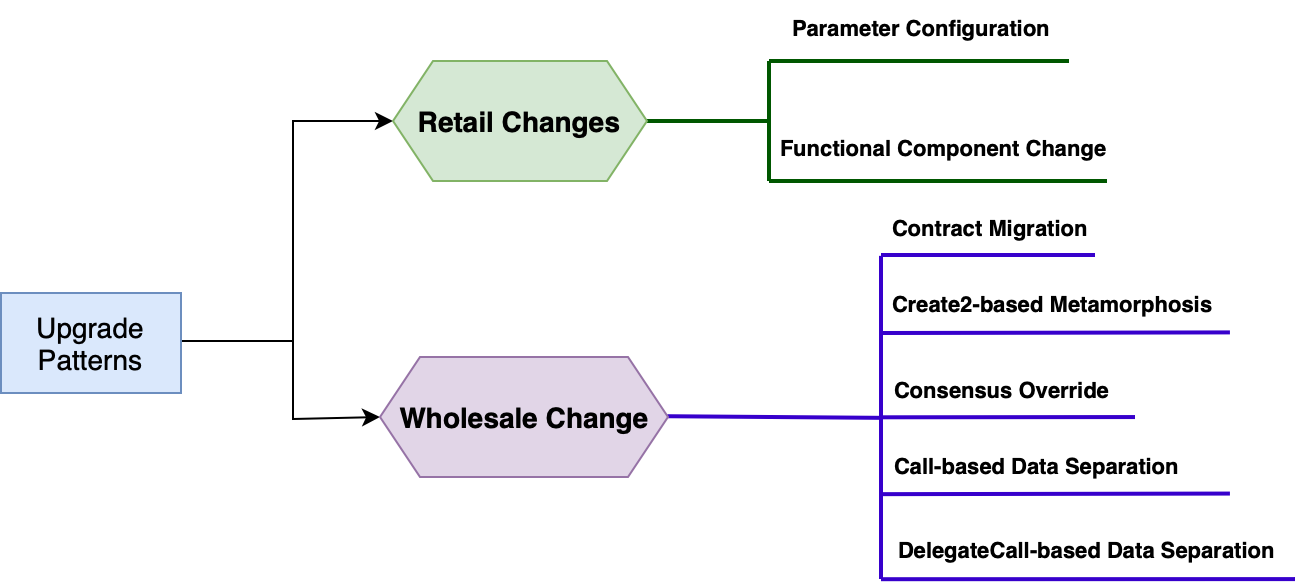
\includegraphics[width=0.8\textwidth]{figures/New_Classification.png}
  \caption{Classification of upgradeability patterns.\label{fig:class}}
\end{figure}

A variety of upgradeability patterns have been proposed for smart contracts. Most leverage Ethereum-specific operations and memory layouts and are not applicable to other blockchain systems.


\subsection{Parameter Configuration}
\label{sec:parameter}

We first categorize upgradeability patterns into two main classes: \textit{retail changes} and \textit{wholesale changes}. A pattern for retail change does not enable the replacement of the entire contract. Rather, a component of the contract is pre-determined (before the contract is deployed on Ethereum) to allow future upgrades, and the code is adjusted to allow these changes. 

The simplest upgrade pattern is to allow a system parameter, that is stored in a state variable, to be changed. This requires a \textit{setter function} to overwrite (or otherwise adjust) the variable, and access control over who can invoke the function. For example, in decentralized finance (DeFi), many services have parameters that control fees, interest rates, liquidation levels, \etc Adjustments to these parameters can initiate large changes in how the service is used (its `tokenomics'). A DeFi provider can retain control over these parameters, democratize control to a set of token holders (\eg stability fees in the stablecoin project MakerDao), or lock the parameters from anyone's control. In Section~\ref{sec:governance}, we dive deeper into the question who can upgrade a contract. 

% = = =

\subsection{Functional Component Change}
\label{sec:component}

While a parameter change allows an authorized user to overwrite memory, a functional component change addresses modifications to the code of a function (and thus, the logic of the contract). In the EVM, code cannot be modified once written and so new code must be deployed to a new contract, but can be arranged to be called from the original contract. 

One way to allow upgradable functions is deploying a helper contract that contains the code for the functions to be upgradeable. Users are given the address of the primary contract, and the address of this secondary contract is stored as a variable in the primary contract. Whenever this function is invoked at the primary contract, the primary contract is pre-programmed to forward the function call, using the opcode \texttt{Call}, to the address it has stored for the secondary contract. To modify the logic of the function, a new secondary contract is deployed at a new address, and an authorized set of individuals can then use a parameter change in the primary contract to update the address of the secondary contract.

The DeFi lending platform Compound~\footnote{\url{https://compound.finance}} uses this pattern for their interest rate models~\footnote{\url{https://github.com/compound-finance/compound-protocol/blob/v2.3/contracts/InterestRateModel.sol}} which are tailored specifically for each asset. The model for one asset can be changed without impacting the rest of the contract~\cite{openzeppelinPost}.

Upgradeable functional components need to be pre-determined before deploying the primary contract. Once the primary contract is deployed, it is not possible to add upgradeability to existing functions. It also cannot be directly used to add new functions to a contract. Finally, this pattern is most straightforward when the primary contract only uses the return value from the function to modify its own state. Thus, the function is either `pure' (relies only on the parameters to determine the output) or `view' (can read state from itself or other contracts, but cannot write state). If the function modifies the state of the primary contract, the primary contract must either expose its state variables to the secondary contract (by implementing setter functions), or it can run the function using \texttt{Delgatecall} if the secondary contract has no state of its own. 

This upgrade pattern suggests a way forward for wholesale changes to the entire contract: create a generic ``proxy'' contract that forwards all functions to a secondary contract. To work seamlessly, this requires some further engineering (Sections~\ref{sec:callbased} and \ref{sec:delegatecall}).


\subsection{Consensus Override}
\label{sec:hardfork}

The two previous patterns enable portions of a smart contract to be modified. The remaining patterns strive to allow an entire contract to be modified or, more simply, replaced. The first wholesale pattern is not a tenable solution to upgradeability as it as only been used rarely under extraordinary circumstances, but we include it for completeness. 

Immutability is enforced by the consensus of the blockchain network. If participating nodes (\eg miners) agreed to suspend immutability, they can in theory allow changes to a contract's logic and/or state. If agreement is not unanimous, the blockchain can be forked into two systems---one with the change and one without. In 2016, a significant security breach of a decentralized application called ``the DAO'' caused the Ethereum Foundation to propose overriding the immutability of this particular smart contract to reverse the impacts of attack. In the unusual circumstances of this case, it was possible to propose and deploy the fix before the stolen ETH could be extracted from the contract and circulated. Nodes with a philosophical objection to overriding immutability continued operating, without deploying the fix, under the name Ethereum Classic.

% = = =

\subsection{Contract Migration}
\label{sec:migration}

The simplest wholesale upgrade pattern is to deploy a new version of the contract at a new address, and then inform users to use the new version---called a ``social upgrade.'' One example is Uniswap\footnote{\url{https://uniswap.org}}, which is on version 3 at the time of writing. Versions 1 and 2 are still operable at their original addresses. 

Contract migration does not require developers to instrument their contracts with any new logic to support upgradeability, as in many of the remaining patterns, which can ease auditability and gas costs for using the contract. However for most applications, there will be a need to transfer the data stored in the old contract to the new one. This is generally done in one of two ways. The first is to collect the state of the old contract off-chain and load it into the new contract (\eg via its constructor). If the old contract was instrumented with an ability to pause it, this can eliminate race-conditions that could otherwise be problematic during the data migration phase. The second method, specific to certain applications like tracking a user's balance of tokens, is to have the user initiate (and pay the gas) for a transfer of their balance to the new contract.
 
 % = = =

\subsection{\texttt{CREATE2}-based Metamorphosis}
\label{sec:metamorphic}

Is it possible to do contract migration, but deploy the new contract to the \textit{same} address as the original contract, effectively overwriting it? If so, developers can dispense with the need for a social upgrade (but would still need to accomplish data migration). At first glance, this should not be possible on Ethereum, however a set of opcodes can be ``abused'' to allow it: specifically, the controversial\footnote{\href{https://www.reddit.com/r/ethereum/comments/lx32kv/expectations\_for\_backwardsincompatible\_changes/}{``Expectations for backwards-incompatible changes / removal of features that may come soon.'' V. Buterin, Reddit r/ethereum, Mar 2021.}} \texttt{SELFDESTRUCT} opcode and the 2019-deployed \texttt{CREATE2}. 

Consider a contract, called Factory, that has the bytecode of another contract, A, that Factory wants to deploy at A's own address. \texttt{CREATE2}, which supplements the original opcode \texttt{CREATE}, provides the ability for Factory to do this and know in advance what address will be assigned to contract A, invariant to when and how many other contracts that Factory might deploy.  The address is a structured hash of A's ``initialization'' bytecode, parameters passed to this code, the factory contract's address, and a salt value chosen by the factory contract.\footnote{Specifically: $\mathsf{addr} \leftarrow \mathcal{H}(\mathtt{0xff} \| \mathsf{factoryAddr} \| \mathsf{salt} \| \mathcal{H} (\mathsf{initBytecode} \| \mathsf{initBytecodeParams}))$} Most often, A's initialization bytecode contains a copy of A's actual code (``runtime'' bytecode) to be stored on the EVM, and the initialization code is prepended with a simple routine to copy the runtime code from the transaction data (calldata) into memory and return. Importantly, however, the initialization bytecode might not contain A's runtime bytecode at all, as long as it is able to fetch a copy of it from some location on the blockchain and load it into memory. In order for \texttt{CREATE2} to complete, the address must be empty, which means either (1) no contract has ever been deployed there, or (2) a contract was deployed but invoked \texttt{SELFDESTRUCT}.

Assume the developer wants to deploy contract A using metamorphosis and later update it to contract B.\footnote{\href{https://medium.com/@0age/the-promise-and-the-peril-of-metamorphic-contracts-9eb8b8413c5e}{``The Promise and the Peril of Metamorphic Contracts.'' 0age, Medium, Feb 2019.}} The developer first deploys a factory contract with a function that accepts A's (runtime) bytecode as a parameter (which includes the ability to self destruct). The factory then deploys A at an arbitrary address and stores the address in a variable called codeLocation. The factory then deploys a simple `transient' contract using \texttt{CREATE2} at address T. This contract performs a callback to the factory contract, asks for factory.codeLocation, and copies the code it finds there into its own storage for its runtime bytecode and returns. As a consequence, A's bytecode is now deployed at address T. 

To upgrade to contract B, the developer calls \texttt{SELFDESTRUCT} on A. Mechanically, the consequences of \texttt{SELFDESTRUCT} on the EVM are only realized at the end of the transaction. In a followup transaction, the developer calls the factory with contract B's bytecode. The factory executes the same way placing a pointer to B in factory.codeLocation. Importantly, it generates the same address T when it invokes \texttt{CREATE2} since the `transient' contract is identical to what it was the first time---this contract does not contain contract A or B's runtime code, it just contains abstract instructions on how to load code. The result is contract B's runtime bytecode being deployed at address T where contract A was. 
  

As it is concerning that a contract's code could completely change, we note that metamorphic upgrades can be ruled out for any contract where either: it was not created with \texttt{CREATE2}, it does not implement \texttt{SELFDESTRUCT}, and/or its constructor is not able to dynamically modify its runtime bytecode. 

% = = =

\subsection{\texttt{CALL}-based Data Separation}
\label{sec:callbased}

To avoid migrating the stored data from an old contract to an upgraded contract, a contract could instead store all of its data in an external ``storage'' contract. In this pattern, calls are made to a ``logic'' contract which implements the function (or reverts if the function is not defined). Whenever the logic contract needs to read or write data, it will call the storage contract using setter/getter (aka accessor/mutator) functions. An upgrade consists of (1) deploying a new logic contract, (2) pausing the storage contract, (3) granting the new logic contract access to the storage contract, (4) revoking access from the old contract, and (5) unpausing the storage contract. 

An important consideration is that the layout of the storage contract cannot be changed after deployment (\eg we cannot add a new state variable). This can be side-stepped to some extent by implementing a mapping (key-value pair) for each primitive data type. For example, a new uint state variable can be a new entry in the mapping for uints. This is called the Eternal Storage pattern (ERC930). It however requires that every data type be known in advance, and is challenging to use with complex types (\eg structs and mappings themselves).

A variant of this pattern can introduce a third kind of contract, called a proxy contract, to address the social upgrade problem. In this variant, users permanently use the address of the proxy contract and always make function calls to it. The proxy contract stores a pointer (that can be updated) to the most current logic contract, and asks the logic contract to run the function using \texttt{CALL}. Unlike the functional component pattern (Section~\ref{sec:component}), the proxy will catch and forward \textit{any} function (including new functions deployed in updated logic contracts) using its fallback function.  With or without proxies, this pattern is very powerful, but instrumenting a contract to use it requires deep-seated changes to the contract code. As our measurements will show, it has fallen out of favour for the cleaner \texttt{DELEGATECALL}-based pattern (Section~\ref{sec:delegatecall}) that addresses the same issues with simpler instrumentation. 


% = = =

\subsection{\texttt{DELEGATECALL}-based Data Separation}
\label{sec:delegatecall}

This pattern is a variant on the idea of chaining each function call through a sequence of three contracts: proxy, logic, and storage. The first modification is reversing the sequence of the logic and storage contracts: a function call is handled by the proxy which forwards it to the storage contract (instead of the logic contract). The storage contract then forwards it to the logic contract using \texttt{DELEGATECALL} which fetches the code of the function from the logic contract but (unlike \texttt{CALL}) runs it in the context of the contract making the call---\ie the storage contract. When upgrading, a new logic contract is deployed, the proxy still points to the same storage contract, and the storage contract points to the new logic contract. Since the proxy and storage contracts interact directly and are both permanent, the functionality of both can be combined into a single contract. It is common for developers to call this the `proxy contract,' despite it being a combination of a proxy and a storage contract. 

This pattern is generally cleaner than using the previous \texttt{CALL}-based pattern because the logic contract does not need any instrumentation added to it. It is an exact copy of what the contract would look like if the upgrade pattern was not being used at all. However this does not mean the pattern in a turn-key solution. Each new logic contract needs to be programmed to respect the existing memory layout of the storage contract, which has evolved over the use of all the previous logic contracts. The logic contract also needs to be aware of any functions implemented by the storage contract itself---if the same function exists in both the storage contract and the logic contract (called a function clash), the storage function will take precedence.


The main issue with function clashes is that the proxy contract needs, at the very least, to provide an admin (or set of authorized parties) the ability to change the address of the logic contract it delegates to. This can be addressed in four main ways:

\begin{enumerate}

\item Developers are diligent that no function signature in the logic contract is equal to the signature of the upgrade function in the proxy contract (note that signatures incorporate a truncated hash of the function name, along with the parameters types, so collisions are possible). 

\item As found in the \emph{universal upgradeable proxy standard (UUPS)} (EIP-1822): implement the upgrade function in the logic contract, which will run in the context of the proxy contract. Its exact function signature must be hardcoded into the proxy contract. Every logic contract update must include it or further updates are impossible.

\item As found in the \textit{beacon proxy} pattern (EIP-1967): deploy another contract, called the beacon contract, to hold the address of the logic contract and implement the setter function for it. The proxy contract will get the logic contract address from the beacon every time it does a \texttt{DELEGATECALL}. The admin calls the beacon contract to upgrade the logic contract, while normal users call the proxy contract to use the DApp. 

\item As found in the \textit{transparent proxy} pattern (EIP-1538): inspect who is calling the proxy contract (using \texttt{msg.sender()})---if it is the admin, the proxy contract catches the function call and if it is anyone else, it is passed to the proxy's fallback function for delegation to the logic contract. 

\end{enumerate}

A drawback of the entire \texttt{DELEGATECALL}-based pattern is that logic contracts need to be aware of the storage layout of the proxy contract. In a stand-alone contract, the compiler (\eg Solidity) will allocate state variables to storage locations, and using \texttt{DELEGATECALL} does not change that, however new logic contracts need to allocate the same variables in the same order as the old contract, even if the variables are not used anymore. This can be made easier with object-oriented patterns: each new logic contract extends the old contract (inheritance-based storage). Other options include mappings for each variable type (eternal storage) or hashing into unique memory slots (unstructured storage). The \textit{Diamond Storage} pattern (EIP-2535) breaks the logic contract into smaller clusters of one or a few functions that can be updated independently, and each can request one or more storage slots in a storage space managed by the proxy contract itself. 


\section{Evaluation Framework}
\label{app:eval}

% !TEX root = ../main.tex

    



\begin{table*}[ht!]

    \renewcommand{\arraystretch}{1}
    
    
    \begin{tabular*}{0.9\textwidth}{@{\extracolsep{\fill}} lcccccccccccc}
    
    \textit{Method} &
    \headrow{Can replace entire logic} & 
    \headrow{No need to migrate state from old contract} &  
    \headrow{User endpoint address unchanged} &
    \headrow{No need to instrument source} &
    \headrow{No need to deploy a new contract to upgrade} &
    \headrow{No indirection between contracts} & 
    \headrow{No downtime to upgrade} &
    \headrow{No function selector clashes} &
    \headrow{No storage clashes} & 
    \headrow{ } & 
    \headrow{ } \\ \hline 
    
    Parameter Configuration 	&	  &\full&\full&\full&\full &\full&\full&\full&\full&&\\
    Component Change 	        &	  &\full&\full&\prt	&      &\prt &\full&\full&\full&&\\
    Contract Migration			&\full&     &     &\full&	   &\full&\full&\full&\full&&\\ 
    Create2 metamorphosis 		&\full&     &\full&\full&      &\full&	   &\full&\full&&\\
    Call-based 		            &\full&\full&     &     &	   &	 &\full&\full&\full&&\\ 
    DelegateCall-based 			&\full&\full&\full&\prt	&	   &     &\full&     &     &&\\ \hline 
    \\
                                                                                        
    \end{tabular*}
    
    \caption[Evaluation of Upgradeability Patterns]{An evaluation of upgradeability patterns. \full~ indicates the upgrade method is awarded the benefit in the corresponding column. \prt~partially awards the benefit. Empty cells shows that the method does not satisfy the property.} 
    \label{tab:eval}
    \end{table*}
      





%%%%%%%%%%%%%%%%%%%%%%%%%%%%%%%%%%%%%%%%%%%%%%%%%%%%%%%%%%%%%%%%%%%%%%%%%%%%%%%%%%%%%%%
%%%%%%%%%%%%%%%%%%%%%%%%%%%%%%%%%%%%%%%%%%%%%%%%%%%%%%%%%%%%%%%%%%%%%%%%%%%%%%%%%%%%%%%




In this section, we compare and evaluate different methods discussed in previous section and explain the consequences regarding each method to the users and developers of Dapps.
Table~\ref{tab:eval} summarizes the pros and cons of each upgradeability pattern, omitting consensus override as it is only used in emergencies. The detail of criteria and properties that are used to assess each method, and also take-aways from the evaluation are described in further sections.

\subsection{Properties}

There are some characteristics that can help the designer to decide which method should be used on the system and add upgradeability to the Dapp. In this part we pencil out these criteria and evaluate different methods based on these criteria. In this part we describe and specify what it means that each row of our table receives a full dot (\full), partial dot (\prt), or nothing. 

\subsubsection{Can replace entire logic}
An upgradeability method in which the admin is able to replace the entire logic of the system earns a full dot (\full) otherwise it receives nothing.

\subsubsection{No need to migrate state from old contract}
In some patterns, there is no need to collect data from the old version and push it to the new contract which receive a full dot (\full). On the other hand, patterns which required to migrate data from old version receive nothing.

\subsubsection{User endpoint address not changed}
In some upgradeability methods, after the upgrade process, users must call a new contract address to use the Dapp. It is equivalent to having 2 different Dapps at the end of the upgrade. Alice uses Dapp X which uses one of the upgradeability patterns at address A before the upgrade. After upgrade, she may be unaware that upgrade happened and use the previous address (receive full mark (\full)) or she may need to use address B instead which receive nothing.

\subsubsection{No need to instrument source}
Upgradeability patterns in which the developers do not need to change any part of the original code to add the upgrade method receives nothing. The methods in which the developers do not need to change the whole code but should add a proxy contract or change just one component of the system receive half dot (\prt) and patterns in which the developers should change the whole code to add upgradeability receive full mark (\full).


\subsubsection{No need to deploy a new contract}
In some upgradeability patterns, the admin needs to deploy a new smart contract in the process of upgrade which receives nothing. Upgradeability methods which do not need to deploy a new contract for the process of upgrade receive a full dot (\full).

\subsubsection{No indirection between contracts}  
Indirection happens if the first external message need be forwarded from a contract to another using one of the \texttt{CALL}, \texttt{STATICCALL}, or \texttt{DELEGATECALL} opcodes. Upgradeability methods that do not need any indirections receive a full dot (\full). An upgradeability pattern that contains indirections which adds an extra gas because of adding one or more layers of indirection awarded nothing. An upgradeability method in which not all but just a portion of the incoming transactions need indirection receive half dot (\prt). 


\subsubsection{No downtime to upgrade}
Patterns which have a downtime of the Dapp in the upgrade event receive full dot (\full) otherwise it receives nothing. 

\subsubsection{Function Selector Clashes}
Upgradeability methods in which the developer should take care of function selector risks due to the using of \texttt{DELEGATECALL} opcode receive full dot (\full), otherwise receive nothing. 

\subsubsection{Storage Clashes}
Upgradeability methods in which the developer should take care of storage clashes risks in two contracts due to the using of \texttt{DELEGATECALL} opcode receive full dot (\full). 



%%%%%%%%%%%%%%%%%%%%%%%%%%%%%%%%%%%%%%%%%%%%%%%%%%%%%%%%%%%%%%%%%%%%%%%%%%%%%%%%%%%%%%%%%%%%%%%%%%%
%%%%%%%%%%%%%%%%%%%%%%%%%%%%%%%%%%%%%%%%%%%%%%%%%%%%%%%%%%%%%%%%%%%%%%%%%%%%%%%%%%%%%%%%%%%%%%%%%%%

\subsection{Evaluation Framework: Take-Aways}
\label{app:eval2}

In this section we discuss about the consequence of each upgrade methods regarding the criteria we mentioned in the previous part for users and developers that want to use the upgradeability pattern or uses a Dapp that uses one of the mentioned patterns.

\subsection{Speed of an Upgrade}
Upgrade events of a Dapp consists of two different processes. First a way to come to an agreement for changing the system, and then a way to implement and execute the change. The First part depends on the reason behind the upgrade. If the upgrade is to patch a bug, then the process to come into agreement is very fast but if the goal behind upgrade is to add new functionality or change a logic, it usually starts with a proposal and after some discussions, if the agent that responsible for the decision agree with the proposal, the execution part will be started. We won't discuss the first process because it depends on the type of agent discuss in \ref{sec:governance}.
After coming into agreement about the change, the speed that the admin can implement and execute the upgrade depends on three criteria discussed above: \textit{No need to deploy a new contract to upgrade}, \textit{No need to migrate state from old contract}, and \textit{having a downtime in the upgrade process}.

\textit{Parameter change} method is the fastest way to execute the upgrade because there is no need to deploy a new contract, and no need to migrate state and no downtime in the system.
\textit{Component change} method change is not as fast as parameter change method but faster than other types because the admin needs to deploy a specific smart contract which is a small component of the system and also update an address variable inside the main contract that points to that specific component and change it to the address of the new version of that component. But there is no need to migrate data and there is no downtime needed for this upgrade method.

\textit{Migration} method has a slow upgrade process. The reason is that the admin needs to deploy a new contract and also the admin or users should transfer the data from old version to the newer version. In most migration processes the developer team deploy a \textit{Migrator} contract and users should use this Migrator contract to withdraw their funds/data from the previous version and move it to the newer version. But, there is no downtime in the Dapp and no need to change a state variable.

\textit{Call-based} and \textit{DelegateCall-based} are very similar to each other in the speed of upgrade. These two are not as quick as \textit{Retail changes} because the developer needs to implement and deploy the \textit{whole logic} contract to the blockchain and then change the pointer addresses inside the storage/proxy contract to the newer version.
On the other hand these two approaches are faster than \textit{Migration} because as mentioned before, there is no need to migrate data. There is no downtime in these methods.

\textit{Metamorphic} method is the slowest way to upgrade a system which uses this method because similar to the migration plan there is a need to deploy a contract and migrate the state to the newer version but there is a difference between these two. In metamorphic method, the admin first should \textit{Self-Destruct} the previous version in a single transaction and after that transaction send a contract creation transaction to deploy the newer version. Because self-destruct happened at the end of the transaction, the process of upgrade happens on two different transactions which is a downtime to the system. This downtime could be a gap between order of the two transaction in a single block or could be gap between blocks that these two transactions included into blockchain. 


\subsection{Cost of Upgrade}

One of the main differences between upgradeability approaches is how much does the upgrade process costs for the admins and users. The cost of upgrade mostly depends on two criteria explained above: 1) no need to deploy a new contract, 2) no need to migrate a the state to newer version.

\textit{Parameter change} method is the cheapest method in the upgrade event because there is no need to deploy a new contract or migrate data.
\textit{Component change} is in the middle, because there is a need to deploy a new contract (however it is cheaper comparing to methods in which we should deploy the whole logic), but there is no need for data migration.
\textit{Migration} plan is very expensive in the upgrade event because we need to deploy a new contract and migrate the data from the old version which is very expensive.
\textit{Call-based} and \textit{DelegateCall-based} are very similar to each other in the cost of upgrade which is more expensive than component change, but cheaper than migration. In both the admin must deploy the a contract containing the whole logic, but there is no need to migrate the whole data.
\textit{Metamorphic} method is the most expensive method we have because we need to deploy a new contract, migrate data to the newer version and also we need to self-destruct the previous version before the upgrade event which adds cost to the upgrade process.


\subsection{Gas overhead for users}
Sometimes in upgradeability patterns, we have a tradeoff between adding a feature to the pattern to improve it and increasing the cost (gas needed for the transactions) for users that want to interact with our Dapp.

In patterns that needs indirection, such as \textit{Call-based}, \textit{Delegatecall-based}, and \textit{Component change} pattern an extra cost will be added to the users, because for all or some of the transactions to the Dapp, our system needs to forward the calls to another contract using Call or Delegatecall opcode to the users. 
Also in \textit{Delegatecall-based} pattern to mitigate the function selector clashes or storage clashes, we need to add some other checks to our code which also increases the cost of interacting with the Dapp.
Also there are some other ideas that addresses some limitations of one type of upgradeability pattern, but increases the cost for users. For instance, in \textit{Call-based} approach one of the problems is that after upgrade users should use a new address for using the Dapp but adding a \emph{Registry} contract can help to mitigate this. Using Registry contract, all other contracts should ask the registry to find out the latest version of the contract and then calls to the newer version which adds a gas cost to the users. 

\subsection{Useability}
Upgradeability patterns differ in term of Useability and it depends on three criteria explained above; \textit{User endpoint address unchanged}, \textit{No need to migrate state from old contract} and \textit{Downtime in upgrade events}.

Patterns in which the endpoint address is changing after upgrade event, \textit{Migration} and \textit{Call-based} is not user friendly because each time that the upgrade happens, the user must use the newer address. So there is need to make awareness about this address change which is a hard action and need to socially interact with the all users and make them aware of the change. We have two main type of users in the Dapp ecosystem, normal user or another smart contract (Dapp) that uses our system. Regular users which uses the official interface (website) of the project may do not sense any changes, but users that work with the smart contract directly or via their own interface (e.g, Centralized Exchanges), or other Dapps that uses the smart contract must have a way to upgrade the address they uses to use the newer version and if they did not implement a way to upgrade this address then their Dapp will face problems. So these patterns are make problems for composability of the ecosystem.

In most of \textit{Migration} plan upgrade events, users are responsible for the migration of their data using a migrator contract (for instance, the user must withdraw the fund and use a migrator contract to push the data into the newer version) which add costs to the user and it is not user friendly. This is one reason that make the migration plans very hard because some users are not doing the process of migration and stay on the previous version which is like having a fork for the Dapp in side of the Dapp team (e.g, Uniswap V2 and V3).
In \textit{Metamorphic} pattern as mentioned before there is a downtime during the upgrade. So users cannot work with the Dapp on that exact time which is not user friendly.


\subsection{Dealing with two different new versions}
In \textit{Migration} and \textit{Call-based} pattern we will come up with two different Dapps after each upgrade event. So, a decision must be made for the previous version. One possible choice could be shutting down the old version. It can be done by self-destructing the old version, or by having a pausing mechanism to stop the older version functionality. In migration plan it is not regular to stop the previous version because in most migration plans, users are responsible to move their funds and data from the previous version to the new one and we cannot force them to do that, so we cannot stop the smart contract. 
The other option could be having a mechanism that after the upgrade, all calls to the previous version just be forwarded to the newer version which add costs and have some limitations like we cannot call the new functions defined in the newer version using the old version. This option is doable in Call based patterns. The other problem of this option is that if we upgrade a system more than one time then the calls to the first version should be redirected through lots of contracts to reach to the newer version. Also it adds complexity because developers must maintain more than one contract~\cite{tobBlogPost}.


\subsection{System Complexity} \label{sysComplexity}

Using upgradeability patterns will add to complexity of our system but the degree of complexity varies and depends on the pattern. 
\textit{Parameter Change} method does not change the system in general but just adding a mechanism to change pre-specified variables in the system. The most important issue about this pattern is that the developer team must limit the boundary of these parameter for the security of the system. For instance in MakerDao platform~\footnote{\url{https://makerdao.com/}}, Stability fee is changeable but if this variable be changed to 100\% then the whole system will be halted, so it should be limited.
\textit{Component Change} pattern is very similar to the parameter change, but a whole component could be changed and finding the safe boundary of changes and limiting this boundary is a bit harder.
\textit{Migration} plans for upgradeability does not change any complexity to the system because we do not need to change any part of system to add this type of upgradeability to it. The only important issue regarding this pattern is that we must be sure that there is a way to collect data from the old version like having getter functions for reading data and also having a withdraw function for users to collect data and funds from previous version and push or deposit it to the newer version.
Using \textit{Call-based} patterns adds higher degree of complexity to the system compared to previous patterns. As discussed before, in this pattern we must be sure that the storage and logic contract is divided and there is not any storage variable inside the logic contract. This is one of the main security issues that found in the Dapps using this pattern regarding Trail of Bits company reports~\cite{tobBlogPost}. To add a way in storage contract to define new variables, developers uses the eternal Storage pattern for their storage contract which is very hard to apply for complex data structures in Ethereum such as mappings or structures. This is another source of complexity using Call-based pattern.
\textit{Delegate-call} pattern adds complexity to the code because of using \textit{Delegate-call} opcode in its logic. As mentioned above because of using this opcode, the developer should take care of storage clashes and also function selector clashes. Other than these two there are some other limitations and risks of using this patterns. For instance, we cannot have a \textit{Constructor} function on the logic contract, because constructor functions is used to initialize specific variables at deployment time and if we have a constructor inside the logic, then storage of implementation contract will be changed and not storage of proxy contract. To mitigate this problem we can add a regular function named \textit{Initialize} function inside the implementation and make sure that this function can be called \emph{once} to act just like a constructor function. 
\textit{Metamorphic} pattern is proposed recently and not well-tested yet. There are some risks to this pattern as well. We should be sure that we have a mechanism to self-destruct the contract. Otherwise we cannot redeploy a new version and so our contract won't be upgradeable. The other important issue related to Metamorphic pattern is that the developer must know that each time they want to upgrade the system the whole storage will be wiped out and need to re-initiate the whole state after re-deployment. 

%%%%%%%%%%%%%%%%%%%%%%%%
%%%%%%%%%%%%%%%%%%%%%%%%

\section{Finding Upgradeable Contracts} 
\label{sec:proxyFinding}

We now design a series of measurement studies to shed light on the prevalence of the various upgrade patterns. We exclude retail changes from our measurements, because variable changes and external function calls are too commonplace to distinguish. We focus on wholesale patterns, and devote the most effort to finding contracts using the \texttt{DELEGATECALL}-based data separation pattern (Section~\ref{sec:delegatecall}) as these are the most widely used and there are various sub-types (UUPS, beacon, \etc). The other types of wholesale patterns are: 
\begin{itemize}
\item \textbf{Consensus override:} Only 1 occurrence to date (the DAO attack~\cite{dhillon2017dao}).
\item \textbf{Contract migration:} Not detectable in code; relies on social communication of the new address.
\item \textbf{\texttt{CREATE2}-based metamorphosis.} Already measured by Frowis and Bohme~\cite{frowisnot} in a broader study of all uses of \texttt{CREATE2}. They found 41 contracts between March 2019 and July 2021 that upgraded using this pattern.
\item \textbf{\texttt{CALL}-based data separation.} We conducted a quick study of 93K contracts with disclosed source code~\cite{smart_contract_sanctuary}. We identified the Eternal Storage pattern using regular expressions and found 140 instances, the newest having been deployed over 3.5 years old. We conclude this pattern is too uncommon today to pursue a deeper bytecode-based on-chain measurement.  
\end{itemize}


\subsection{Methodology} 

\begin{figure}[t!]
 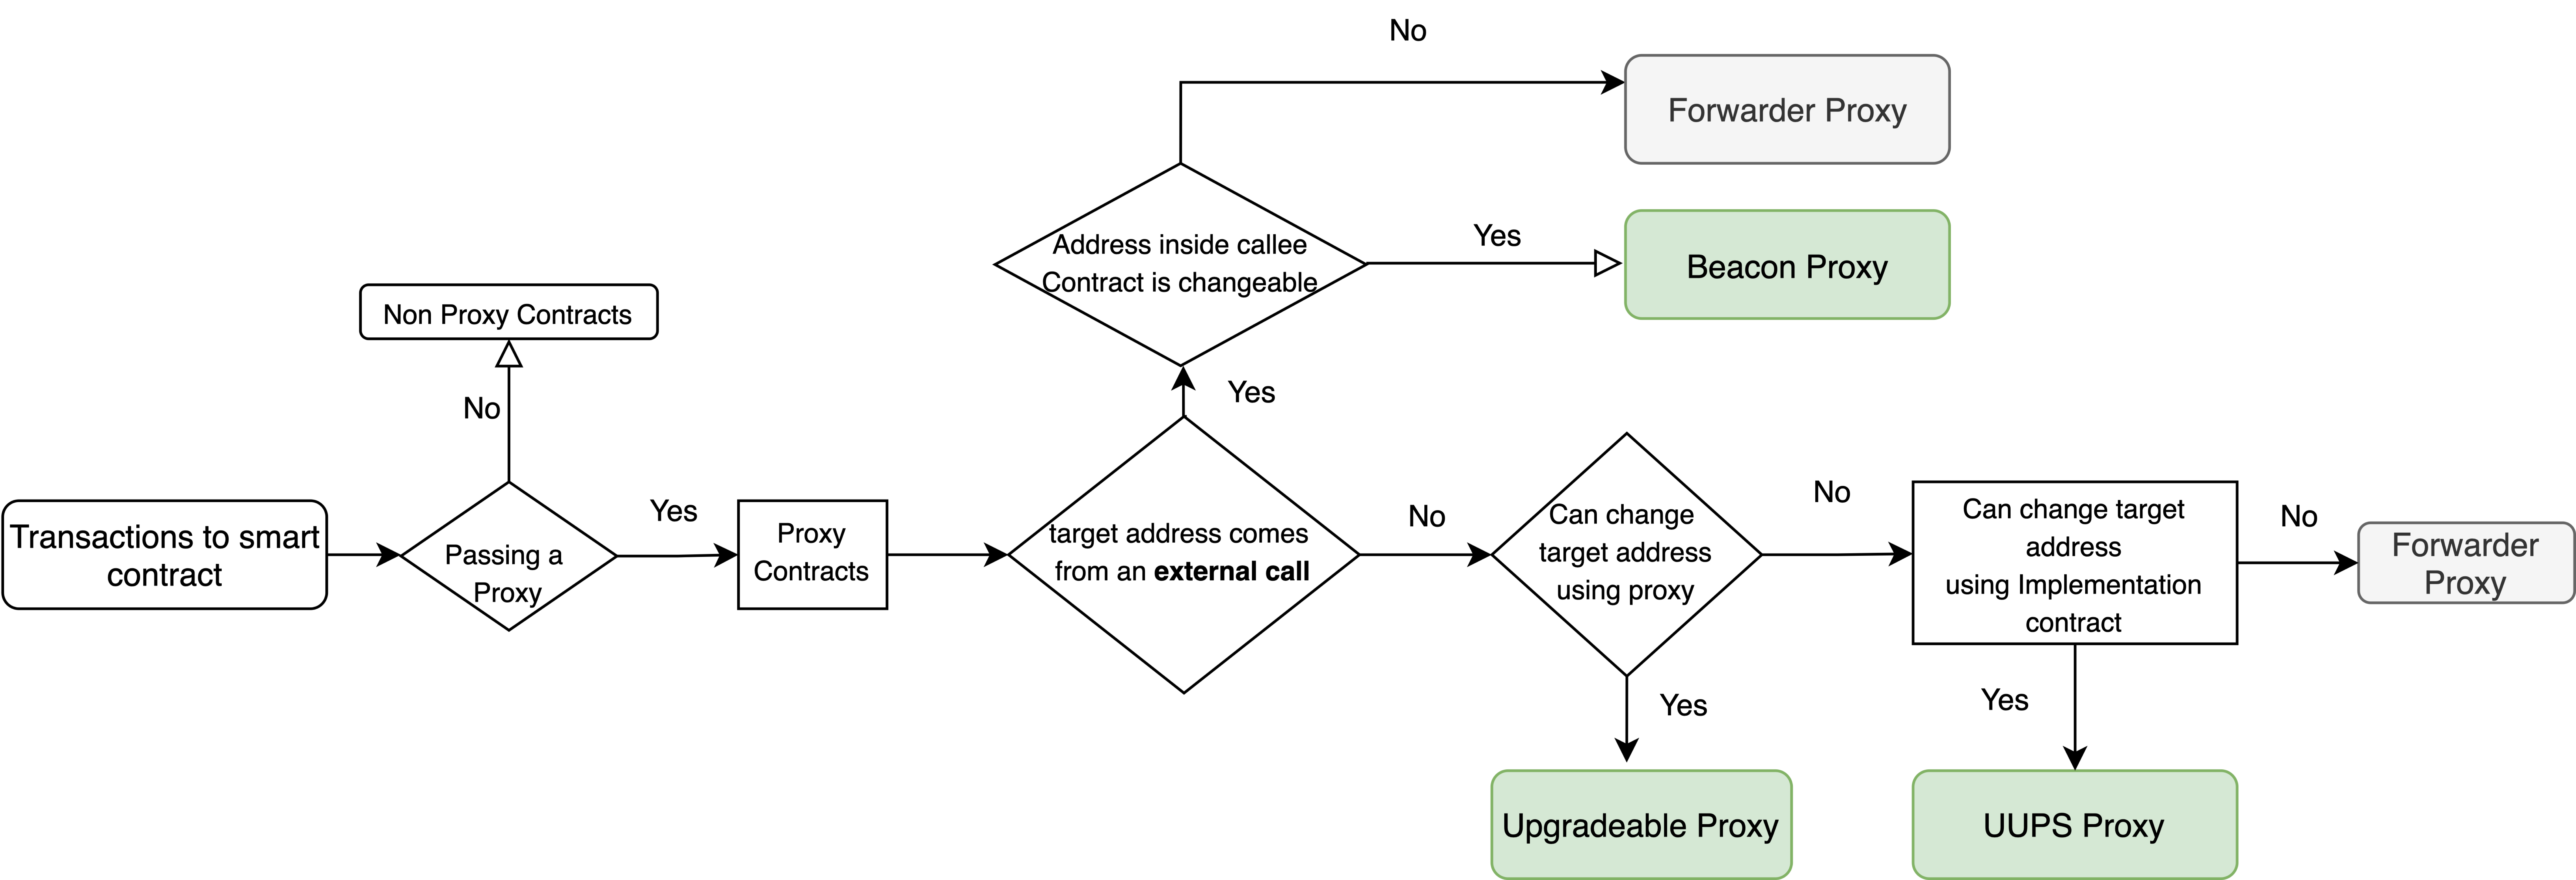
\includegraphics[width=1\textwidth]{figures/New-method.png}\label{flowchart}
 \caption{Flowchart for distinguishing upgradeable contracts (green) from forwarders, and for determining the upgradeability pattern type.}
\end{figure}

% % %

\paragraph{Finding proxies.} While not every use of a proxy contract is for upgradeability (\eg minimal proxies~\cite{minimalProxy}, \texttt{DELEGATECALL} forwarders~\cite{delegatecallForwarders}, \etc), all \texttt{DELEGATECALL}-based upgradeability variants have the functionality of a proxy. We therefore start by measuring the number of contracts with a proxy component, and then filter out the \textit{Forwarders} which do not enable upgradeability. To identify proxies, we examine every \texttt{DELEGATECALL} action and see if it was proceeded by a call with an identical function selector to the contract making the \texttt{DELEGATECALL} action, which indicates   the contract does not implement this function and instead caught it in its fallback function, and is now forwarding it to another contract at, what we will call, the \textit{target address}. We used an Ethereum full archival node\footnote{\url{https://archivenode.io/}} and replayed each transaction in a block to obtain Parity VM transaction traces. \texttt{DELEGATECALL} is one \texttt{callType} of an \texttt{action} within a trace. Specifically, if the data of two consecutive actions of a transaction are equal and a \texttt{DELEGATECALL} is in the second action, it shows that the transaction passes the fallback function (if any other function in the contract is called, other than fallback, then the first four bytes of the data will be changed). The \texttt{DELEGATECALL} indicates the fallback transferred the whole data to the target address without altering it, which means the contract implements a proxy.

\paragraph{Distinguishing forwarders and upgradeability patterns.} In an upgradeable contract, the target address for the \texttt{DELEGATECALL} must be modifiable. If it is fixed, we tag it as a forwarder. We define five common patterns for determining the target address cannot be changed:

\begin{enumerate}
 \item The target address is hardcoded in the contract.
 \item The target address is saved in a constant variable type.
 \item The target address is saved in an immutable variable type and the deployer sets it in a constructor function.
 \item The target address is defined as an unchangeable storage variable.
 \item The proxy contract grabs the target address by calling another contract but there is no way the callee contract can change this address.
\end{enumerate}

In the first three situations, the target address will be appeared in the runtime bytecode of the contract. For every proxy-based \texttt{DELEGATECALL}, we obtain the target address from the transaction's \texttt{to address}, and we obtain the caller's bytecode by invoking \texttt{eth\_getCode} on the full node. If we find the target address in the bytecode, we mark it as a forwarder. 

In the fourth case, we find where the target address is stored by the contract by decompiling the contract, with \textit{Panoramix}\footnote{\url{https://github.com/palkeo/panoramix}}, locating the line of code in the fallback function that makes the \texttt{DELEGATECALL}, and marking the storage slot for the target address. We parse the code and check if an assignment to that slot happens in any function in the contract. The process is explained in Section~\ref{app:assignment} in detail. If any assignment is found, we should be sure that the other variable assigned to the target address variable comes from the input of that function. If these conditions are satisfied, there is a function inside the contract that can change the target address and we mark the proxy as an upgradeable proxy contract. 

Recall in the Universal Upgradeable Proxy Standard (UUPS) pattern, the logic contract implements a function to update the target address that is run in the proxy contract's context using \texttt{DELEGATECALL}. This is a sub-case of the fourth case, where we check the logic contract instead of the proxy contract. If we determine the logic contract can assign values to the logic contract in any function, we tag it as UUPS.

In the fifth case, we rewind the transaction trace from the proxy-based \texttt{DELEGATECALL} and look for the target address being returned to the proxy contract in another action. If we find it being returned by a contract, we apply the methodology from the fourth case to this contract. If the target address is modifiable, we mark it as using the Beacon proxy upgradeability pattern. All contracts that remain after performing all of the checks above are marked as forwarders. 


 %%%%%%%%%%%%%%%%%%%%%%%%%%%%%%%%%%%%%%%%%%%%%%%%%%%%%%%%%%%%%%%%%%%%%%%%%%%%%%%%%%%%%%%%%%%%%%%%%%%%%%%%%%%%%%%%%%%%%%%%%%%%%%%%%%%%%%
 \subsection{Assignment Checker Module}
\label{app:assignment}

\begin{figure}[t!]
 \centering
 \includegraphics[keepaspectratio,height=20cm, width=30cm]{figures/Upgradeability_finder-3.png}
 \caption{Upgradeability Proxy Contract Finder}
 \label{fig:finderModule}
\end{figure}

The whole measurement process is depicted on figure~\ref{fig:finderModule}. We need a module to check whether the admin can change target address on the proxy contract,using a function in the proxy contract, implementation contract or beacon contract. For this purpose the module must get the \textit{Bytecode} of the proxy,implementation or beacon address as input and find the variable name and also its storage slot of the target address. Then checks to find out is there any function inside the contract that gives the admin the ability to change the target address.

We use bytecode decompiler named \textit{Panoramix decompiler} \footnote{\url{https://github.com/palkeo/panoramix}} to decompile the bytecode into well-formatted python language codes. The decompiled code gives us all storage variables of the related contract and the storage slots of those variables in a function named \textbf{Storage}. On the other hand, the decompiled code will tell us if a function is \textit{Payable} or not. Among these Payable functions the one that does not have name or its name is fallback is the \textit{fallback} function of the contract. So we will try to find the line of code that \textit{Delegate Call} happened on it and collect these lines. Now that we have storage variable names and storage slots of these variables and also the line of code inside fallback that have the delegatecall, we will check to find the target address variables. We are doing that by checking if one of the storage variables inside Storage function is used in the line of code that contains delegate call. We will add them to an array of implementation addresses.

There is two other steps here. First finding other variable names with the same storage slots as the implementation addresses we found from the first step by checking the Storage function and also finding another variables that being assigned to those implementation variables in some other part of the code. We will add these two type of variables to the implementation addresses as well.

Now that we have a list for implementation addresses, we will search through the code to find if any assignment happened to one of them. If yes we will pick the variables that is assigned to target variable and then check if this assignment happened in a specific function and to one of the inputs of that function. In this case this function will be the upgrade function because the caller of this function can upgrade the target address by calling this function with desired input. 

To summarize what we did, we find all possible variables in the code that can change the target address inside the contract and check if there is any function inside them that can assign new address to the target address variable.

The whole process is depicted on figure~\ref{assignmentFinder}.

\begin{figure}[t]
 \centering
 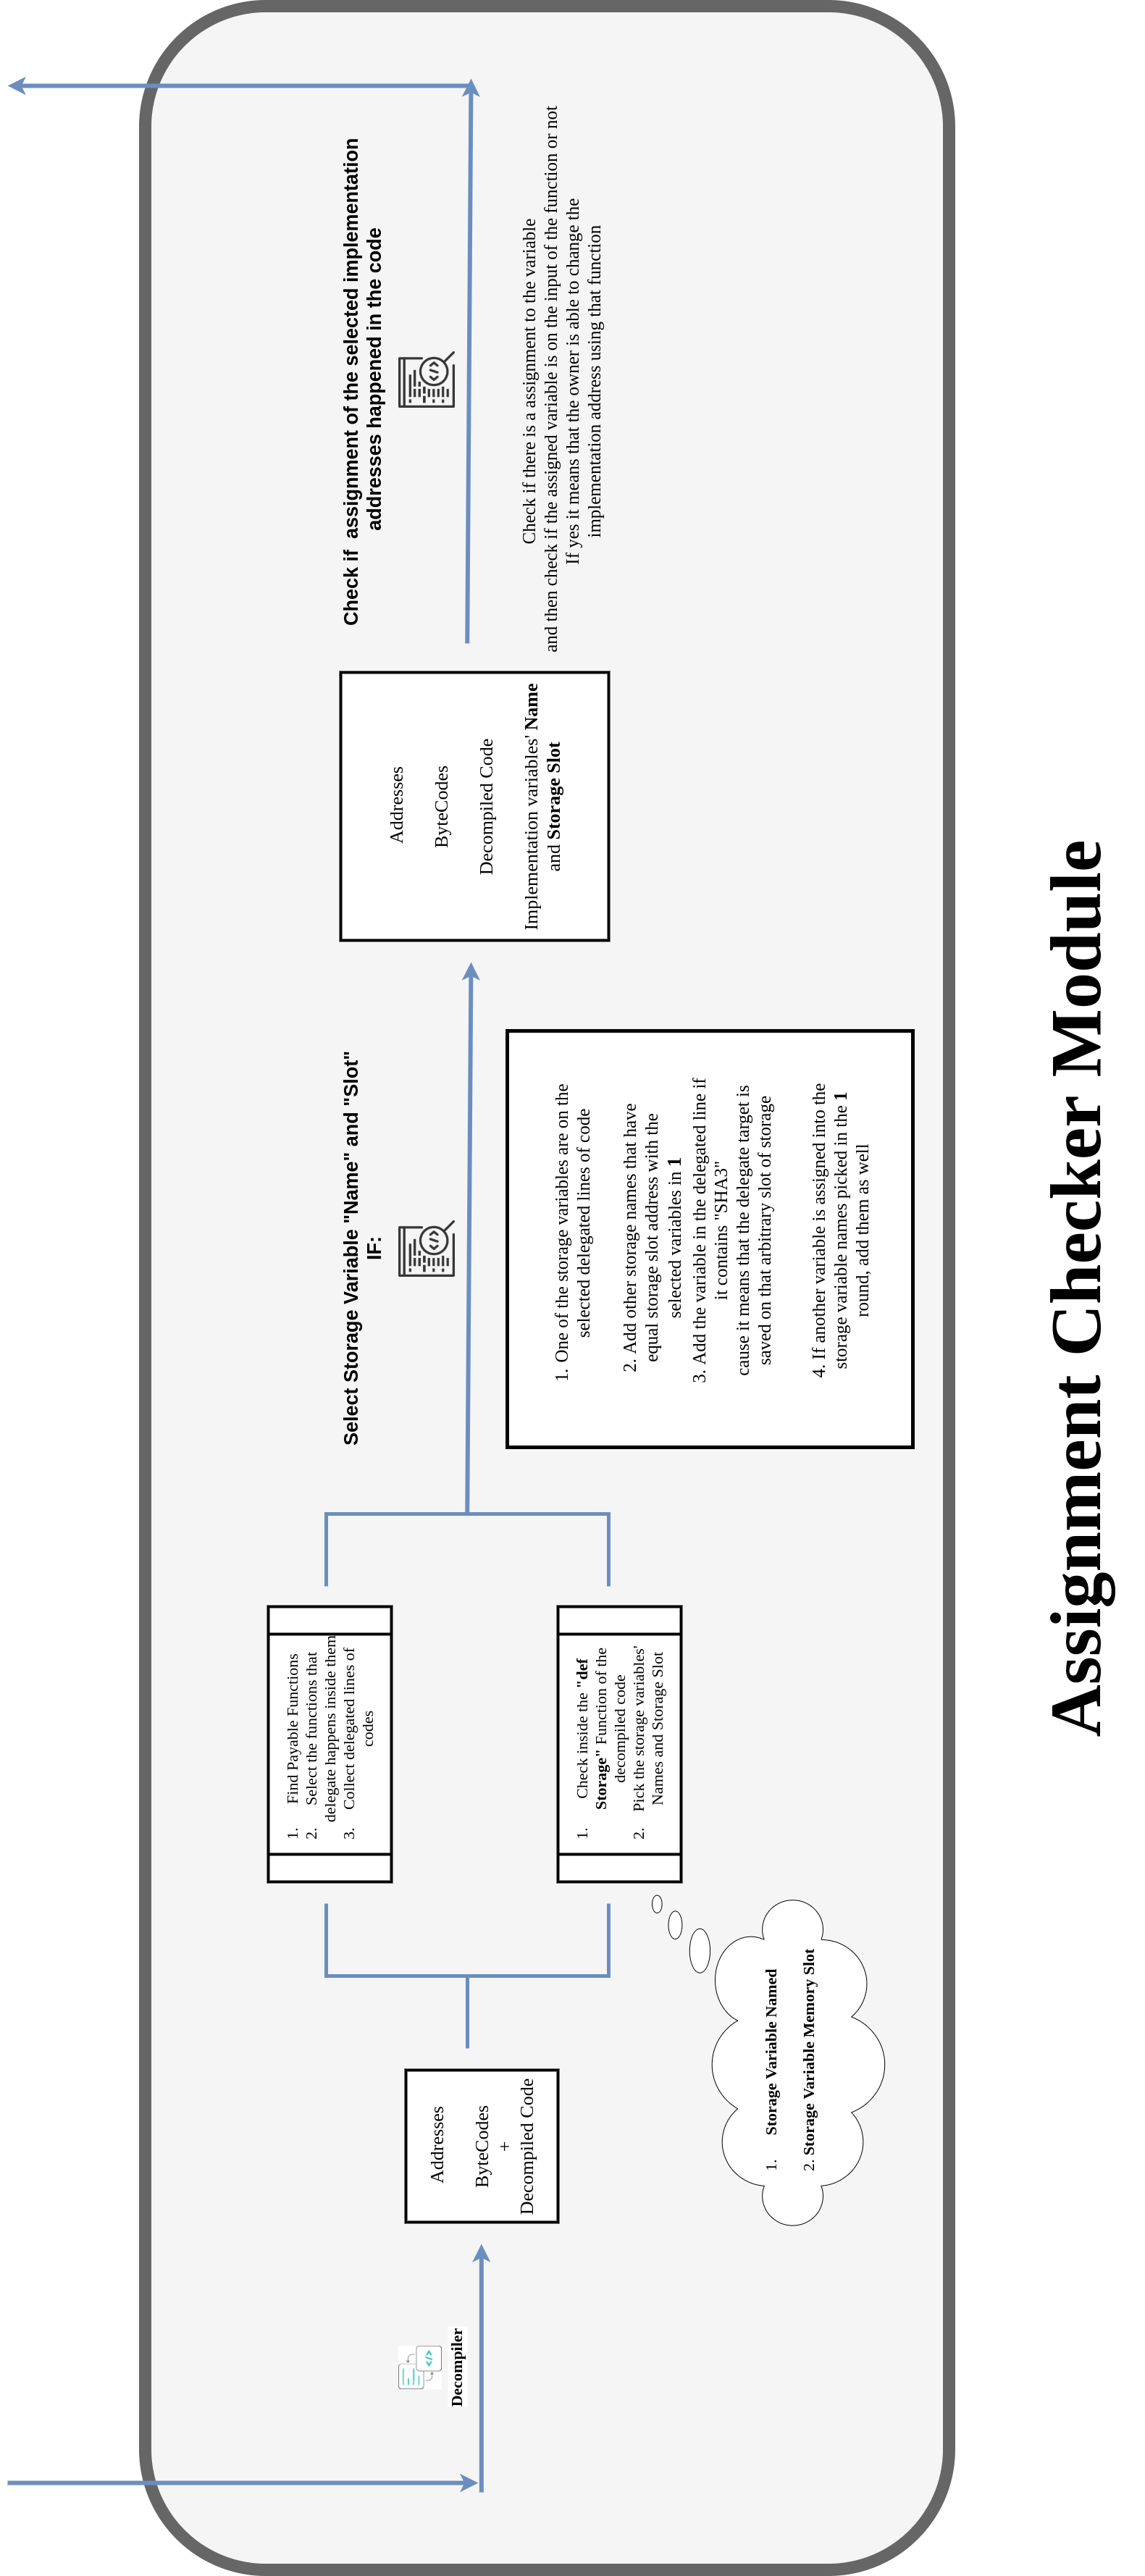
\includegraphics[keepaspectratio,height=20cm, width=30cm]{figures/Assignment_finder.png}
 \caption{Assignment CheckerModule}
 \label{assignmentFinder}
\end{figure}

 %%%%%%%%%%%%%%%%%%%%%%%%%%%%%%%%%%%%%%%%%%%%%%%%%%%%%%%%%%%%%%%%%%%%%

 \subsection{Results}

 \begin{table}[t]
 \centering
 \begin{tabular}{|l|r|}
 \hline
 Proxy Contracts (Total) & 1,427,215  \\ \hline 
 Proxy Contracts (Filtered) & 13,088  \\ \hline 
 Regular Upgradeable Contracts & 7,470  \\ \hline
 UUPS & 403  \\ \hline
 Beacon & 352  \\ \hline
 \end{tabular}
 \caption{\label{tab:updata} Results of each \texttt{DELEGATECALL}-based upgrade pattern for the time-period {Sep-05-2020} to {Jul-20-2021} (2,064,595 blocks).}
 \vspace{-10pt}
 \end{table}
 
 Our measurements cover block number \texttt{10800000} to \texttt{12864595}, which corresponds to the time-period \texttt{Sep-05-2020} to \texttt{Jul-20-2021}, and are reported in Table~\ref{tab:updata}. While we found 1.4M unique proxy contracts, many of these share a common implementation contract and are part of the same larger upgradable system. As one example, the NFT marketplace OpenSea~\footnote{\url{https://opensea.io}} gives each user a unique proxy contract. After clustering contracts, we find 13K unique systems.  
 
 For the 8,225 upgradeable systems (regular, UUPS and beacon), we randomly sampled 150 contracts and manually verified they were upgradeable proxy contracts. We also sampled 150 contracts from the forwarders to verify they are not upgradeable, however we did find 2 false-negatives. Our model did not catch these contracts because a failure happened when decompiling them and our assignment checker detector in turn failed. Note that for UUPS contracts, the implementation contracts are much larger and harder to analyze than the proxy contract itself.


 %%%%%%%%%%%%%%%%%%%%%%%%
 %%%%%%%%%%%%%%%%%%%%%%%%

 \section{Finding the Admin}
\label{sec:governance}

If a contract is upgradeable, someone must be permissioned to conduct upgrades. We call this agent the admin of the contract. In the simplest case, the admin is a single Ethereum account controlled by a private signing key, called an externally owned account (EOA). A breach of this key could lead to malicious updates, as in the case of the lending and yield farming DeFi service Bent Finance ~\cite{bentFinanceHack}. Bent Finance deployed a \textit{Transparent Upgradeable Proxy} with an EOA admin that was breached (unconfirmed if via an external hack or insider attack). The EOA pushed an updated logic contract\footnote{\url{https://etherscan.io/address/0xb45d6c0897721bb6ffa9451c2c80f99b24b573b9}}  which moved tokens valued at \$12M USD into the attacker's account\footnote{0xd23cfffa066f81c7640e3f0dc8bb2958f7686d1f} and then upgraded the logic contract to a clean version to cover-up the attack. Based on \textit{The State of DeFi Security 2021}~\cite{certikReport} report by Certik,\footnote{\url{certik.com}} ``centralization risk'' is the most common attack vector for hacks of DeFi projects. 
 
Control over upgradeability typically falls into one of three categories: 

\begin{enumerate}
\item \textbf{Externally owned Address (EOA):}
One private key controls upgrades. It is highly centralized and one malicious admin or compromised private key could be catastrophic. It is also the fastest way to respond to incidents. An EOA may also pledge to delegate their actions to an off-chain consensus taken on any platform, such as verified users on \textit{Discord} or \textit{Snapshot}, however with no guarantee they will abide by it. In our measurements, we cannot distinguish this subtype as these are off-chain, social arrangements. 

\item \textbf{Multi-Signature Wallet:}
Admin privileges are assigned to a multi-signature wallet, requiring transactions signed by at least $m$ of a pre-specified $n$ EOAs.   This distributes trust, and tolerates some corruption of EOAs or loss of keys. There is no guarantee different EOAs are operated by different entities and may be security theatre put on by a single controlling entity.

\item \textbf{On-Chain Governance Voting:} A system issues a governance token and circulates it amongst its stakeholders. Updates are decided through a decentralized voting scheme where the weight of the vote from an EOA (or contract address) is proportionate to how many tokens it owns. This system is potentially highly decentralized, but the degree depends on the distribution of tokens (\eg if a single entity controls a majority of tokens, it is effectively centralized). Voting introduces friction: (1) a time delay to every decision---some critical functionality might bypass the vote and use quicker mechanisms (\eg global shutdown in MakerDAO), and (2) on-chain network fees for each vote cast.

\end{enumerate}

\subsection{Methodology}

We conduct our measurement on the 7,470 regular upgradeable contracts from Section~\ref{sec:proxyFinding}. The process can be divided into two main parts: finding the admin account's address and finding the admin type (EOA, multi-sig, or decentralized governance).

\paragraph{Finding the admin account's address.} EIP-1967 suggests specific arbitrary slots for upgradeable proxy contracts to store the \textit{admin address}.\footnote{Storage slot 0xb53127684a568b3173ae13b9f8a6016e243e63b6e8ee1178d6a717850b5d6103} We first check this specific storage slot using \texttt{eth\_getStorageAt} on the full node. If it is non-zero, we mark what is stored as the admin address. 
For non-EIP-1967 proxies, we use a process that is very similar to how we found the storage slot of the target address in Section~\ref{sec:proxyFinding}. We first find the function in which the admin can change the \textit{target address} (upgrade function). This function is critical and should only be called by the admin. We extract the access control check and mark the address authorized to run this function as the admin address.

\paragraph{Finding the admin type.} Having the admin address, we can check if the account is an EOA by invoking \texttt{eth\_getCode} on the address from the full node: if it is empty, it is an EOA. Otherwise, it is a contract address. The most common multisig contract is Gnosis Safe.\footnote{\url{https://gnosis-safe.io/}} We automatically mark the admin type as multi-sig if we detect Gnosis safe. We then switch the manual inspection to find other multi-signature wallets (\eg MultiSignatureWalletWithDailyLimit, \etc) and add them to the data set. 

In some cases, the admin address is itself a proxy contract---a pattern known as an Admin Proxy. This adds another layer of indirection. We are reusing our methodology for identifying proxy contracts to exact the real admin account, and the proceed as above. Further details of the methodology and implementation are provided below:

\subsubsection{EIP-1967.}
As mentioned above EIP-1967~\footnote{\url{https://eips.ethereum.org/EIPS/eip-1967}} suggested specific arbitrary slots for upgradeable proxy contracts to store implementation contract's address and \textit{Admin address}\footnote{Storage slot 0xb53127684a568b3173ae13b9f8a6016e243e63b6e8ee1178d6a717850b5d6103 for admin}.

In first step we use \textit{eth\_getStorageAt} method of an Ethereum full archival node to search the EIP-1967 specified storage slot for admins on our 7,470 proxy contracts. If the result of this method is non-zero it means that the proxy uses EIP-1967 standard because the specified storage slot is an arbitrary slot and one can store variable in this slot just by defining this slot which means that they used EIP-1967.

So, for non zero results, we capture the address which is the address of admin of the proxy. Now we try to find the type of these admin addresses. Having the address of the admin we use \textit{eth\_getCode} method to check the code of the admin account. If the code is empty, it means that this account is not a smart contract so it is an EOA. we find \textit{900} EOA admins that their proxy uses EIP-1967 standard.

The remained admin addresses are contract because their account keeps code. This contract can be multi signature smart contract wallets. The most widely used multi signature wallet is Gnosis Safe\footnote{\url{https://gnosis-safe.io/}} wallets. We automatically checked if the code of the admin address is the Gnosis wallet multi signature patterns. After picking Gnosis safe wallets we manually checked \%10 of the remained addresses to find if they used other patterns for their multi signature wallet and we found some other patterns (e.g. MultiSignatureWalletWithDailyLimit, etc.). After Finding all these types we checked the admin codes to see whether they are multi signature wallets. We find \textit{255} admin accounts that uses multi signature wallets as their admin.

There is another class of admin contracts named \textit{Admin Proxy} contracts. These admin proxy contracts are another layer of re-direction between the real admin and the Dapp's proxy contract. The admin proxy contracts are proxy contracts that redirect the messages from the real admin into the Dapp's proxy. The only person who can use admin proxy is the admin (a.k.a owner) of the admin proxy. So we first filter the admin proxy contracts using the codes we get from the previous part and then try to find the owner of the admin proxy contracts. The owner of admin proxy contract (the real admin) also can be EOA, Multi-sig or governance contract. Finding the owner of the admin proxy contract, we used \textit{eth\_getCode} method to check the code of these account and find out if they are EOAs or Multi-signatures or governance schemes. Doing this we find \textit{1202} EOA admin accounts and \textit{567} multi signature admins. We marked the remained proxy admin addresses as Governance/Not Known admin types and we have \textit{462} of them. There were also non admin proxy contracts which use EIP-1967 but they were not EOA or Multi signatures. We marked them as Governance/Not Known admin types and we have \textit{53} of them.

\subsubsection{Non EIP-1967.}
For proxy contracts which not use EIP-1967, the problem is we don't know where the admin address is saved in the proxy contract's storage (what is the storage slot of the admin address). It can be saved in a storage slot of the contract or be hardcoded in the smart contract\footnote{There are some other possible ways to store the admin address for instance saving it in another contract and each time make an external call to get the address but to our knowledge this pattern is not widely used as a standard}. 

So there are two ways that the admin address is saved in the proxy contract. It can be saved as a storage variables or it can be hardcoded as a fixed address.

In storage variable case, the first question is in which storage slot the admin address is stored. So, the first step is to find the storage slot of the admin address variable. Also for the fixed address we should find the fixed address of the admin directly.

To find the slot of the storage variable in which admin address is saved, we first find the function in which the proxy can be upgraded. For finding the upgrade function we exactly do what we did in \ref{sec:proxyFinding} part. We first find the storage variable in which we saved the implementation address and then we find a function in which the implementation address can be changed using the inputs of that specific function. 

The upgrade function of a proxy contract is a critical function and the only account that can call this function should be the admin of the proxy contract. So, there should be an access control check inside the upgrade function to check whether transaction sender is equal to the admin address or not.
So, after finding the upgrade function we search for conditionals that checks the caller of the transaction and by doing that we can find the admin address or the storage variable in which the admin address is stored.


If the admin address is stored in a storage variable, then we should find the storage slot of that specific storage variable. For finding the storage slot we do what we did in \ref{sec:proxyFinding} part by using \textit{def storage} function of the decompiler and check the storage slot of the storage variable we found, and the admin address is saved on it. 
Now we have the storage slot of the admin address and we should start doing all the things we did for EIP-1967 in the previous part. 
In the EIP-1967 the storage slot for admin address was pre-specified and we do not need to find the slot but in this case we use the above methodology to find the slot but the further steps are the same as EIP-1967.
So, by using the \textit{eth\_getCode} method for admin address inside the storage slot we find above, we can check wether the admin is EOA, Multi-sig, Governance, Proxy admin or not known.
In this part we find \textit{1313} EOA addresses and \textit{104} multi-sig admins. Also by checking proxy admins we find \textit{92} EOA addresses and \textit{16} Multi signatures that uses proxy admin as a level of indirection. 

In another case the admin address may be stored directly in a specific arbitrary storage slots. In this type the compiler will specify the address using the \textit{sha3} hash notation. In this case same as above we find the conditional check on the transaction sender and then find the storage slot in that line and hash of that pre-specified string. 
By finding this arbitrary storage slot and doing the same processes we did in the previous part we find \textit{2} EOA addresses and \textit{10} Multi-sig addresses.

The only case that is left is proxy contracts, in which the address of the admin is hardcoded inside them. It very straight forward. We find the upgrade function and the access control check on the caller of the transaction and then pick the fixed admin address and do the same processes mentioned above to find the admin types. There are \textit{49} EOAs, \textit{36} multi-signature admins and \textit{160} governance and not known admin addresses. 

\subsection{Results}

\begin{table}[t]
\centering
\begin{tabular}{|l|r|r|r|r|r|r|}
\hline      &\multicolumn{2}{c|}{EIP-1967} & \multicolumn{4}{c|}{Non-EIP-1967}         \\
\hline
Type 				& \makecell{Regular\\Admins} & \makecell{Admin\\Proxy} 	& \makecell{Regular\\Admins} 	& \makecell{Admin\\Proxy} & \makecell{Arbitrary\\Slots} &  \makecell{Fixed\\Address}  \\ \hline 
EOA 				& 900  	& 1202		& 1313		& 92			& 2		& 49 		\\ 
Multisig 			& 255  	& 567		& 104		& 16			& 10		& 36		\\ 
Governance/Other 	& 53  	& 462		& 			& 			& 		& 160 	\\ \hline
\end{tabular}
\caption{\label{tab:admindata} Results of each admin type in upgradeable contracts for the time-period {Sep-05-2020} to {Jul-20-2021} (2,064,595 blocks).}
\vspace{-10pt}
\end{table}

Of 7470 proxies, 3558 are controlled by an EOA address, 988 are controlled by a known multi-signature wallet, and 2924 addresses are remaining. Table~\ref{tab:admindata} breaks down each sub-category for these. Of the latter 2924 addresses, these are either decentralized governance or another unknown type. After manual inspection, we note some of the unknown contracts use undefined or new patterns for implementing multi-sig contracts; our model has false negatives in detecting multi-signatures. The results demonstrate significant centralization risk in upgradeability: 48\% of systems could be upgraded with the breach of a single signing key, and an additional 13\% by potentially a small number of signing keys.

%%%%%%%%%%
%%%%%%%%%%


\section{Attacking Universal Upgradeable Proxy Standard (UUPS) contracts} 
\label{sec:attackUUPS}
In this section, we described one of the use-cases of the dataset provided in section~\ref{sec:proxyFinding}. In Section~\ref{sysComplexity}, we discussed that one of the main challenges to the \texttt{DELEGATECALL}-based data separation pattern (Section~\ref{sec:delegatecall}) is that the constructor inside the implementation contract cannot initialize the proxy itself. So instead, there should be a regular function inside the implementation contract named \textit{Initialize} function that can be called just once after deployment by the proxy contract and has the same functionality as the constructor function. Therefore, the contract creator must call the initialize function quickly after deploying the proxy contract. The Initialize function does not have any access control because it is considered to be called once, and this function is responsible for defining the owner. So, before calling this function, the owner's address is not set, and there is no way to have an access control check for the sender. This is why there should be a check to ensure that this function can just be called once at deployment and not after. 
The proxy contract deployer will define and initialize the address of the contract owner via the initialize function. So if the deployer forgets to initialize the contract, any external address can call initialize function and change the owner of the contract to her desired address, and take control of the contract.

The \texttt{Initialize} function can also be called from the implementation contract itself (instead of calling the function by proxy contract). This call will alter the storage of the implementation contract and not the proxy contract. Suppose the deployer forgets to call the \texttt{Initialize} function directly from the implementation contract. Any malicious address can call this function from the implementation contract and change the owner inside the implementation contract, and take control of this contract. 
This malicious actor can change the storage of the implementation contract by calling functions inside it. However, it is not a risk to the system because the proxy contract is responsible for keeping the data in this system and not implementing it. There should be a risk to the system if this malicious actor can change the logic of the implementation contract or self-destruct it. Changing the logic of the implementation contract is not doable in typical cases because implementation contracts are not supposed to be upgradeable. However, there are ways to self-destruct the implementation contract. 

There are two main ways to self-destruct a contract: 1)if the implementation contract has \texttt{SELFDESTRUCT} inside its logic and by calling it. 2)Having a \texttt{DELEGATECALL} or \texttt{CALLCODE} to another contract that has \texttt{SELFDESTRUCT} logic inside~\cite{frowisnot}.

So, we should check if the implementation contract uses \texttt{SELFDESTRUCT} or has \texttt{DELEGATECALL} or \texttt{CALLCODE} to an address that a malicious party can control. If there is a way, the malicious party can self-destruct the implementation contract, and all calls to the proxy will fail. It is a Denial of Service (DoS) attack on the Dapp.
If the Dapp has an upgrade function inside its proxy contract, then the admin of the proxy contract can upgrade into a new version of the implementation contract. This attack was explained in December 2020 by  Trail of Bits team when they audited the code of Aave, a lending project~\cite{aaveBreak}.

Nevertheless, what if the upgrade function is inside the implementation contract and not the proxy contract. As mentioned in Section~\ref{sec:delegatecall}, in UUPS upgradeable contracts, the upgrade function resides in the implementation contract. So there is no way to upgrade the system by the proxy contract. Therefore, if an attacker takes control of the implementation contract by calling the initialize function directly from the implementation contract and then self-destruct it, there is no way to upgrade it. Consequently, the proxy will be locked forever. 
All UUPS contracts that used the Openzepplin UUPS library, whose implementation contact is not initialized, are susceptible to this attack. Because there is a function in the implementation contract of this library named \textit{upgradeToAndCall}, in which the owner can change a target address and then delegate call into the newly changed target address. This attack vector was found in September 2021 and announced by OpenZepplin team~\cite{securityAdvise,uupsAttacks}. There is an easy way to mitigate this attack by calling the initialize function directly from the implementation contract. 

We try to check all UUPS contracts that we find in Section~\ref{sec:proxyFinding} that if any of them can be exploited in this way. We check all of them manually, and the method of checking them is described below:

\begin{enumerate}
\item Check if the implementation contract is not initialized
\item Find initialize function inside the implementation contract
\item check if anybody can call this initialize function directly from the implementation contract and change the owner of the contract
\begin{itemize}
\item Filter those that have a modifier that blocks direct calls to the implementation contract (there is a modifier that just let transactions that come from the proxy contract and blocks direct calls to the implementation contract itself)
\end{itemize}
\item Check if there is a way inside the implementation to self-destruct 
\item Check if there is a function in the implementation contract which has a delegate call to a target address
\item Check if the target address is changeable by a malicious actor
\end{enumerate}

After reviewing the list above, we found 15 contracts in our data set that were exploitable until September 9, 2021. The openzeppelin team patched them by initializing the contract. An attacker could deploy a new malicious contract that executes self-destruct on any calls to it. Then take control of the implementation contract by calling the initialize function them. Afterward, the attacker finds the function inside the implementation contract with a delegate call inside it and finds the target address. There should be a function inside the implementation contract to change the address to the malicious contract that the attacker deployed recently. The attacker calls the function to execute a delegate call into the malicious contract and then self-destruct the implementation contract.

We find 61 UUPS contracts that are not initialized, and anybody can take control of these implementation contracts. However, because these contracts do not use delegate calls or self-destruct, they are not exploitable by this type of attack.

%%%%%%%%%%%%%%%%%%%%%%
%%%%%%%%%%%%%%%%%%%%%%

\section{Concluding Remarks}

In this chapter, we find that \texttt{DELEGATECALL}-based data separation is the most prominent upgrade pattern in Ethereum in recent years. Our evaluation framework gives some hint as to why this is the case. It avoids the need for a social upgrade, as in contract migration or the \texttt{CALL}-based pattern (without a proxy). \texttt{CREATE2}-based metamorphosis was recently made possible (with the introduction of \texttt{CREATE2}) and its use might grow over time, however it shares one major drawback with contract migration: the need to migrate the whole state from the old contract for each update, even if the update is makes minor changes to the logic of the contract. Metamorphic contracts also run the risk of Ethereum removing the \texttt{SELFDESTRUCT} opcode they rely on.  A drawback of \texttt{CALL}-based patterns is the heavy instrumentation each new contract needs before it can be deployed, whereas in a \texttt{DELEGATECALL}-based (along with migration and \texttt{CREATE2}-based) upgrade pattern, developers can simply deploy the new logic contract exactly as it is written. Putting these reasons together, \texttt{DELEGATECALL}-based pattern is an attractive option on balance. 


The main take-away from studying upgradeability on Ethereum is that immutability, as a core property of blockchain, is oversold. Immutability has already been criticized for being dependent on consensus---both technical and social~\cite{walch2016path}---however the widespread use of upgradeability patterns further degrades immutability. Finally, as we show, the prominence of contracts that can be upgraded with a single private key (\ie externally owned account) calls into question how decentralized our DApps (decentralized applications) really are. If the upgrade process is corrupted through a key theft or by a rogue insider, the whole logic of the contract can be changed to the attacker's benefit. 

One recent application of our research was finding all contracts that implement the UUPS upgrade pattern, which become important when a vulnerability was discovered in one of the best-known libraries for implementing UUPS. We describe how we can find potentially vulnerable contracts in Section~\ref{sec:attackUUPS}. While others had found some contracts by looking for specific artifacts left by the UUPS library, we improved the state of the art by looking for the generic pattern of UUPS. 

A final discussion point concerns Layer 2 (L2) solutions, such as optimistic rollups and zk-rollups~\cite{mccorry2021sok}. For the readers that are already familiar with them, their central component is a bridge contract that let computations be performed off of Ethereum (layer 1) and have just the outputs validated on Ethereum. If the bridge contracts is upgradeable, the rules for accepting L2 state are also upgradeable which means every L2 contract is de facto upgradeable even it does not implement an upgrade pattern. We saw Ethereum override the consensus of the network to revert the DAO hack, which was a rare and contentious event. If a similar attack happened on a L2, reverting would be much simpler and not require a hard fork: the L2 could simply update the bridge contract. For this reason, the consensus override upgrade pattern may be less rare in the future. 


\chapter{Oracles: From the Ground Truth to Market Manipulation} \label{ch:oracle}

\textit{
This chapter is adapted from work co-authored by Shayan Eskandari\footnote{Shayan Eskandari and Mehdi Salehi are considered equal first authors} and Catherine Gu, and supervised by Jeremy Clark. It was published at the 2021 ACM Conference on Advances in Financial Technologies (AFT)~\cite{eskandari2021sok}. It appeared as a `systemization of knowledge (SoK)' paper which `are not surveys of prior academic work but rather organization of results presented informally by the open-source community or used in operational projects.'
}

\section{Introduction} \label{sec:intro}

With billions of dollars at stake, decentralized networks are prone to attacks. It is essential that the smart contracts, which govern how systems are run on these networks, are executed correctly. Public blockchains, like Ethereum, ensure the correct execution of smart contract code by taking the consensus of a large, open network of nodes operating the Ethereum software. For consensus to form, many nodes need to make decisions based on the exact same input data. Hypothetically, if a decision requires nodes to fetch data or use a service provider outside of the blockchain, there can be no guarantee that every node in a global network has the same access and view of this external source. For this reason, blockchains only execute on internal sources: data and code provided in a current transaction, or past data and code already stored on the blockchain.

Many potential decentralized applications seem very natural until the designer hits the `oracle problem' and realizes an interface to the external world is required. An oracle is a solution to this problem. It is a service that feeds off-chain data into on-chain storage. The trust model of oracles vary---some data comes with cryptographic certification while other data is assumed to be true based on trusting the oracle, or a set of oracles. Oracle-supplied data cannot easily be changed or removed once finalized on-chain, allowing disputes over data accuracy to be based on a public record. Leveraging this immutability is one approach to incentivizing oracles to post truthful information.

We aim to construct in this chapter a systematization of knowledge (SoK) of implementation choices for oracles, facilitated by breaking down the operation of an oracle into a set of modules. For each module, we explore potential system vulnerabilities and discuss attack vectors. We also aim to categorize all the significant oracle proposals of different projects within a taxonomy we propose. The goal of this SoK is to help the reader better understand the system design for oracles across different use cases and implementations.

\section{Preliminaries}

Ethereum~\cite{wood2014ethereum} is a prominent public blockchain with the largest developer headcount. While oracles are applicable to any blockchain, we will adopt Ethereum as a concrete example of a blockchain for the purposes of explaining each concept in this chapter. Ethereum is inspired by Bitcoin but adds a verbose language for programming \textit{smart contracts} that execute on the \texttt{Ethereum Virtual Machine (EVM)}. All transactions and executions are verified by a decentralized network of nodes. Solidity is the main high-level programming language used by developers for developing smart contracts and decentralized applications (DApps). Smart contracts are small code bases that live on a blockchain. In short, smart contracts can be seen as blackbox applications that get inputs from a user and follow the code flow to the output, which can update the state of the contract and trigger monetary transactions. 

\paragraph{Methodology.} We found papers and other resources by examining the proceedings of top ranked security, cryptography, and blockchain venues; attending blockchain-focused community events; and leveraging our expertise and experience. Our inputs include academic papers, industry whitepapers, blog and social media posts, and talks at industry conferences on blockchain technology, Ethereum, and decentralized finance (DeFi). 


\paragraph{Oracle Use-Cases.} Oracles have been proposed for a wide variety of applications. Based on our reading, most of the use-cases fall into one of the main categories below.

\begin{itemize}

\item \textbf{Stablecoins}~\cite{clark2019sok,MSS20,PHP+19,gu2020empirical,MAKERDAOOracle} and \textbf{synthetic assets}~\cite{SCM21} require the exchange rate between the asset they are price-targeting and the price of an on-chain source of collateral. 
\item \textbf{Derivatives}~\cite{eskandari2017feasibility,biryukov2017findel,synthetix} and \textbf{prediction markets}~\cite{clark2014decentralizing,peterson2015augur} require external prices or event outcomes to settle on-chain contracts.
\item \textbf{Provenance systems}~\cite{RKYCC19,tian2016agri} require tracking information of real world assets like gold, diamonds, mechanical parts, and shipments.
\item \textbf{Identity}~\cite{KL17,maram2021candid} and other on-chain reputation systems require knowledge of governmental records to establish identities.
\item \textbf{Randomness}~\cite{chainlinkvrf} can only be produced deterministically on a blockchain. In order to use any non-deterministic random number, an external oracle is needed to feed the randomness into the smart contract. \textbf{Lotteries}~\cite{pooltogether} and \textbf{games}~\cite{etheroll} are examples. Additionally, cryptographic tools like verifiable random functions (VRF)~\cite{micali1999verifiable,goldbe-vrf-01} and verifiable delay functions (VDFs)~\cite{bunz2017proofs,crypto-2018-28858} can mitigate, respectively, any predictability or manipulability in the randomness.
\item \textbf{Decentralized exchanges} can use prices from an external oracles to set parameters. On-chain market makers~\cite{hertzog2017bancor} uses such prices to minimize the deviation from the external market prices and tailor the pricing function. Additionally, some use oracles to provide sufficient liquidity near the mid-market price for more efficient automated market making~\cite{dodopmm,cofixwhitepaper,cofixblog}.
\item \textbf{Dynamic non-fungible tokens (NFTs)}~\cite{chainlinknft} are crypto-collectables that can be minted, burned, or updated based on external data. For example, sports trading cards which depends on the real-time performance of a player.
\end{itemize}

\section{Related Work}

Given this chapter is a systemization of knowledge (SoK), we will review work on oracles themselves throughout the chapter. In this section, we only discuss other works with a similar goal of providing an overview of different approaches to oracle design, operation, and security. Al-Breiki et al. \cite{al2020trustworthy} present a trust-based categorization of oracle systems, as well as the type of interaction that the on-chain component of the oracle has with the off-chain components. 
Liu and Szalachowski \cite{liu2020first} focus on oracles in the decentralized finance (DeFi) ecosystem, presenting technical architectures and a measurement study on deviations between external market prices and on-chain data from commonly used price oracles.
Lo et al.~\cite{lo2020reliability} propose a framework for assessing the reliability of oracles and ranked them based on the failure probability rate.
Angeris and Chitra \cite{angeris2020improved} analyze the logic behind Automated Market Maker (AMM) projects (\eg Uniswap~\cite{adams2019uniswap} and Balancer~\cite{balancer}) and discuss how these projects could be used as price feeder oracles for other systems.
Williams and Peterson \cite{williams2019decentralized} map oracle systems into two groups---requesters and reporters--- and perform a game theoretical analysis of three defined scenarios between requesters and reporters.

By contrast, in our work, we inspect 17 different oracle systems\footnote{To our knowledge, a much larger set than other research on oracle systems.} and breakdown their design decisions and mechanism implementations (listed in Table~\ref{tab:classification}). We also discuss theoretical and possible attacks on the different building blocks of the oracle systems. Comparatively, we look at a broader types of oracles, including price oracles, binary outcome oracles, and oracle systems, for any type of data such as weather condition information.

% !TEX root = ../main.tex


% = = = = = = = = = = = = = = = = = = = = = = = = = = %
% = = = Modular Work Flow Overview
% = = = = = = = = = = = = = = = = = = = = = = = = = = %

\section{Modular Work Flow} \label{overview_workflow}

% = = = = = = = = = = = = = = = = = = = = = = = = = = %
For our main contribution, we deconstruct how an oracle operates into several modules that generally operate sequentially (but in some solutions, certain steps are skipped) and then we study each module one-by-one. An overview of the work flow is as follows:


\begin{description}
	\item \ref{ground_truth} \textbf{Ground Truth}: The goal of the oracle system is to relay the ground truth (\ie the real true data) to the requester of the data. 

	\item \ref{data_sources} \textbf{Data Sources}: Data Sources are entities that store or measure a representation of the ground truth. There are a diverse set of data sources: databases, hardware sensors, humans, other smart contracts, \etc

	\item \ref{data_feeders} \textbf{Data Feeders}: Data feeders report off-chain data sources to an on-chain oracle system. In order to incentivize truthful data reporting, an oracle system can introduce a mechanism to select data feeders from a collection of available data providers. The incentive mechanism can be collateral-based, such as staking, or reputation-based to find a reliable set of data feeders for each round of selection.
	
	\item \ref{data_feeder_selection} \textbf{Selection of Data Feeders}: The process of determining which data feeders should be used in an oracle system can be categorized into two main types: centralized and decentralized selection.

	\item \ref{aggregation} \textbf{Aggregation}: When data is submitted by multiple data feeders, the final representation of the data is an aggregation of each data feeder's input. The aggregation method can be random selection or algorithmic rule-based, such as using weighted average (the mean) or majority opinion. The design of the aggregation method is one of the most important aspects of an oracle system, as intentional manipulation or unintentional errors during the aggregation process can result in untruthful data reporting by the oracle system.
	
	\item \ref{dispute_phase} \textbf{Dispute Phase}: Some oracle designs allow for a dispute phase as a countermeasure to oracle manipulation. The dispute phase might correct submitted data or punish untruthful data feeders. The dispute phase might also introduce further latency.
	
	\end{description}
	
\begin{figure}[t!]
    \centering
    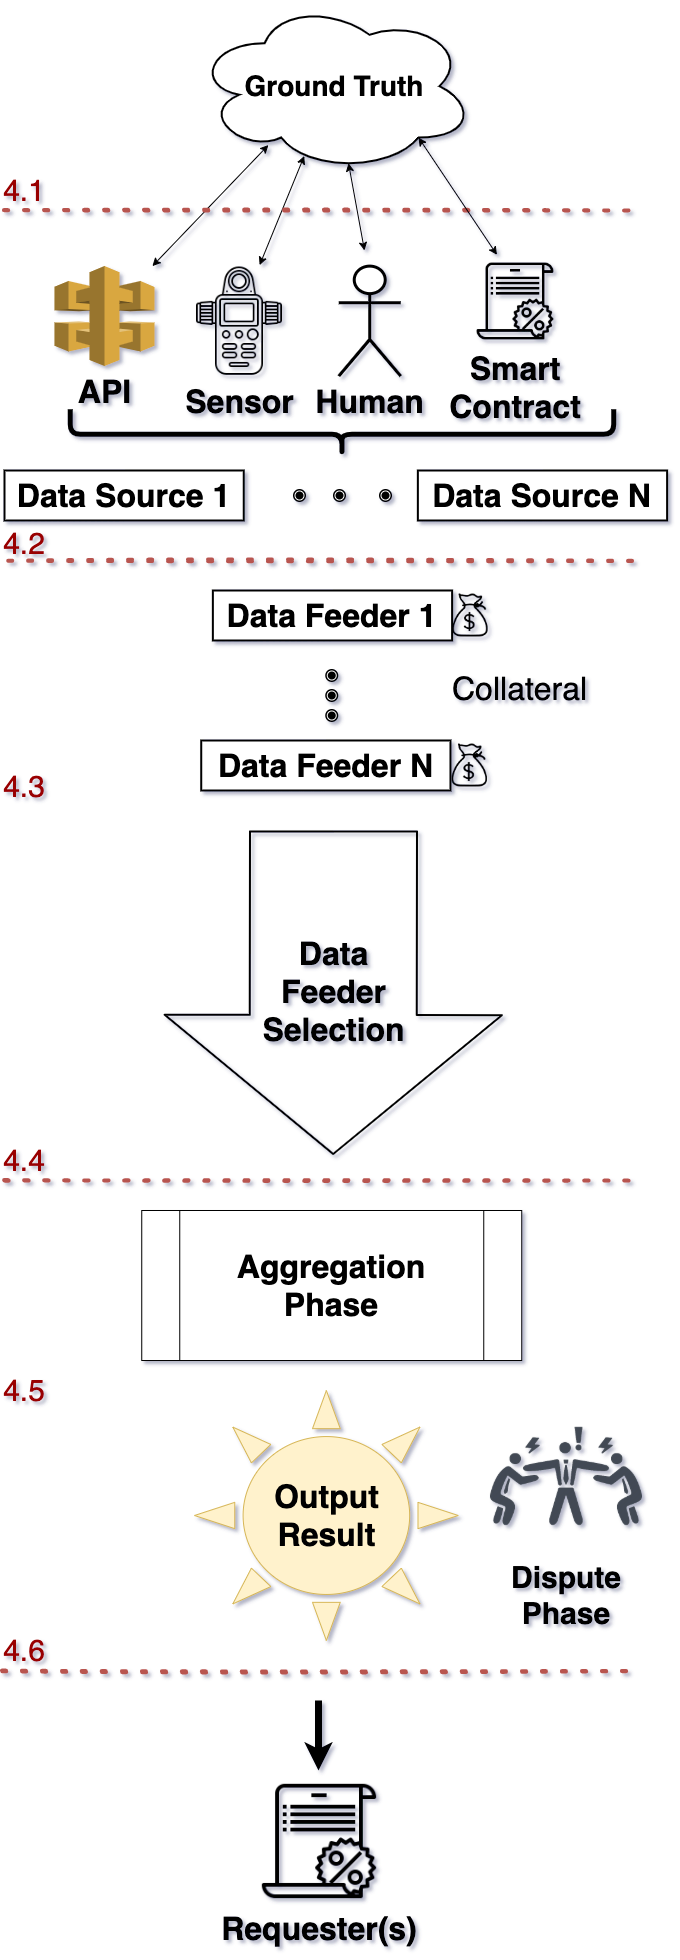
\includegraphics[width=0.35\textwidth]{figures/data_flow_vertical.png}
    \caption[Modular Framework for Oracles]{A visualization of our oracle workflow as described in the text.}
    \label{fig:dataflow}
\end{figure}	
	
	
	
The steps above are visualized in Figure~\ref{fig:dataflow}. Next we dive deeper into the modular workflow by trying to further define each module. As appropriate, we also discuss feasible attacks on the modules and possible mitigation measures.

% = = = = = = = = = = = = = = = = = = = = = = = = = = %
% = = = Ground Truth
% = = = = = = = = = = = = = = = = = = = = = = = = = = %

\subsection{Ground Truth}\label{ground_truth} 

While not a module itself, ground truth is the initial input to an oracle system. Oracle designers cannot solve basic philosophical questions like \textit{what is truth?} However it has to be understood (i) what the data actually represents and (ii) if it is reliable. Data is sometimes sensitive to small details. Consider a volatility statistic for a financial asset: basics like which volatility measure is being used over what precise time period are obvious, but smaller things like the tick size of the market generating the prices could be relevant~\cite{firat2002knowledge}. When data is aggregated from multiple sources, minor differences in what is being represented (called \emph{semantic heterogeneity}) can lead to deviations between values~\cite{madnick2006improving,worboys1991semantic,hakimpour2001resolving}.

While oracle systems will attempt to solve the issue of malicious participants who mis-report the ground truth, it does not address the fundamental question of whether the ground truth itself is reliable. Some philosophers argue truth is observed, and observations require a `web of beliefs' that is subject to error (for its consequences in security, see~\cite{HvO17}). Reliability is judged by the assumptions made about the data source, described next. 

% = = = = = = = = = = = = = = = = = = = = = = = = = = %
% = = = Data Sources
% = = = = = = = = = = = = = = = = = = = = = = = = = = %

\subsection{Data Sources}\label{data_sources}

Data Sources are defined here as passive entities that store and measure the representation of the ground truth. Common types of data sources include \texttt{databases}, \texttt{sensors}, \texttt{humans}, \texttt{smart contracts}, or a combination of them. Depending on how data sources gather and retrieve the ground truth, different attack types arrise. Using a hybrid of data sources (if possible) could reduce the reliability on a single point of input. We describe each common type and their security considerations.

\subsubsection{Humans.}\label{humansDatasource}
A human may provide the requested data, either by direct observation or by indirectly relaying data from another data source. Humans are prone to errors which is the main risk of this data source. Human errors include how the data is retrieved, how the data collector interprets the truth, and if data is relayed from a reliable source. Researchers have categorized human errors into the following three types (from least to most probable): very simple tasks, routine tasks, and complicated non-routine tasks~\cite{lo2020reliability}. An example for each category is, respectably, reading Bitcoin's exchange rate from an unverified source, inputting the data into the system, and configuring the oracle system.

Humans may also act maliciously and deliberately report wrong data when they perceive it will benefit them. As we will see in further modules, a robust oracle system will use incentives and disputes to promote truthful statements. 

% Biases, social engineering

% \todo{add wiki nigeria election problem . also lazy voters, single source of truth (wiki)}
 %Talking about importance of using different data sources ...

% JC: 
% Fake news - what is the oracle angle? how often is a human's perception of the news the input to a smart contract? Seems vaguely related but we need to tighten it if we want to include it. 

% SE: What are the attacks: Look for prediction market attacks and see if anything fits in here. How much does it cost to attack a prediction market? 

\subsubsection{Sensors.} Sensors are electronic devices that collect raw data from the outside world and make it available to other devices. The data source may use more than one sensor to obtain the desired data. One example from traditional finance is the weather derivative, first introduced by the Chicago Mercantile Exchange (CME)~\cite{muller2000weather}. These instruments use weather data provided by trusted institutions, such as the National Climate Data Center,\footnote{\url{https://www.ncdc.noaa.gov/}} which collects weather data through a network of sensors.

Provenance is a highly cited application of blockchain, where products are tagged and traced through out the supply chain, including transportation, for management and/or certification~\cite{tian2016agri,mondal2019blockchain,zelbst2019impact}. The tags could be visual (barcodes) or electronic (RFID). A host of attacks on RFID have been proposed outside of blockchain oracles~\cite{alizadeh2012survey}. Blockchain technology does not solve some important trust issues: ensuring the proper tag is affixed to the proper product, each product has one tag, each tag is affixed to only one product, and tags cannot be transferred between products. This is called the \textit{stapling} problem~\cite{RKYCC19}. 

Sensors can produce noisy data or malfunction. The hardware of a sensor can also be modified when remote or physical access is unauthenticated (or weakly authenticated as many sensors are constrained devices). Probably the highest profile sensor attack (outside of blockchain) is Stuxnet~\cite{langner2011stuxnet}---malware that manipulated the vibration sensors, the valve control sensors, and the rotor speed sensors of Iran's nuclear centrifuges, causing the system to quietly fail~\cite{stuxnetattack}.

\subsubsection{Databases and application programming interfaces (APIs).} % TODO Shayan - Check server/connection section for duplicates - data provision / TLSNotary, etc

The most common mechanism used by software to fetch data is to use an API to obtain the data directly from a centralized database. A database is a set of tables that collect system events, while the API is an interface with the database. For example, a financial exchange keeps track of information in a database about every trade that has been executed. A data source that needs the daily traded volume of an asset could use the appropriate API of the exchange's database to extract the data from the related table in the database.

An active attacker can attack the system from two points. Modifying the data at rest in the database, or modifying the data in transit before and after the API call. 

\subsubsection{Smart Contracts.}

Smart contract could be used as a data source similar to a database. Decentralized finance (DeFi) applications on Ethereum include decentralized exchange services like Uniswap~\cite{adams2019uniswap}, or other oracles that operate on-chain. For instance API3 oracle~\cite{benligiraydecentralized} uses other on-chain oracles, called \textit{dAPIs}, as their data source. These oracles are whitelisted through voting by API3 token holders.

\textit{Automated Market Makers} (AMMs)~\cite{wang2020automated} are an on-chain alternative to centralized exchanges. Liquidity providers collateralize the contract with an equally valued volume of two types of cryptoassets. A mathematical rule governs how many assets of the one type are needed to purchase assets of the other. A well-known example of such mathematical rule is the \textit{Constant Function Market Makers} (CFMM) to calculate the exchange rates of tokens in a single trade~\cite{uniswapexplained}. The idea behind AMM was first raised by Hanson's logarithmic market scoring rule (LMSR) for prediction markets~\cite{hanson2003combinatorial}. A class of DeFi projects (\eg Uniswap~\cite{adams2019uniswap,adams2021uniswap} and Balancer~\cite{balancer}) uses CFMM to automate their market-making process. One of the utilizations of AMM is the ability to measure the price of an asset in a fully decentralized way, which addresses the \textit{pricing oracle problem}~\cite{angeris2020improved}.


% add details and possible attacks (whale attack) for cofixwhitepaper and nestwhitepaper. also include possibility of Oracle malfunction for dodopmm and how it might react to such misinformation - PMM attacks

One potential attack vector to the auto price discovery mechanism in an AMM is to manipulate prices provided by an algorithm, since the algorithmic rules used by an AMM is written in the smart contract and therefore how prices are quoted by the AMM can be calculated in advance. One real case example on \textit{bZx} is described in Section~\ref{oracle_smart_contract}. In addition to market manipulation, \textit{smart contract vulnerabilities}~\cite{atzei2017survey,chen2020survey} could possibly be used to influence the data coming from the Oracle, which we will discuss more in section~\ref{smart_contract}.


% JC: this is described at the end
%Using a real case example, a margin trading DeFi platform, \textit{bZx}, was attacked in what is known as a flash loan attack~\cite{bzxPeckShield,bzxflashloanattack,qin2020attacking}. A flash loan allows anyone to borrow large amounts of crypto funds on leverage at very low cost to execute a series of trades within one atomic transaction so long as the full borrowed amount can be returned at the end of that atomic transaction. In the bZx attack, an adversary executed a trade at an unrealistic price to corrupt the price discovery data on Uniswap, which was then subsequently consumed and used by another DeFi service. The adversary gained more from corrupting the second DeFi service than from losing the trades in the first trade by manipulating the prices. A solution to fix this issue, as implemented in Uniswap V2, is to introduce time frames (TWAP) for price discovery over several blocks (\eg mean price in the last 10 blocks), which mitigates the vulnerabilities caused by flash loans. However, AMM is still nonetheless prone to high-capital market manipulations. % TODO: reduce the size of this paragraph


% = = = = = = = = = = = = = = = = = = = = = = = = = = %
% = = = Data Feeders
% = = = = = = = = = = = = = = = = = = = = = = = = = = %

\subsection{Data Feeders}\label{data_feeders} 

Data feeders are entities who gather and report the data from a data source (Section~\ref{data_sources}) to the oracle system. 
A common configuration consists of an \textit{external feeder} which draws from off-chain data sources and deposit the data to an on-chain module. In case the data source is already on the blockchain, the data feeder step can be skipped.

It is not common to assume data feeders are fully honest, however a variety of threat models exist. Generally, this module will not attempt to determine if the data has been falsified (the later sections data selection (Section~\ref{data_feeder_selection}), data aggregation (Section~\ref{aggregation}) and dispute phase (Section~\ref{dispute_phase}) modules will deal with this issue); rather it will consist of tunnelling the data through the feeder with some useful security provisions. We discuss most important security provisions to achieve data integrity, confidentiality, and non-repudiation on any specific data. 


\subsubsection{Source Authentication.}\label{source_authentication}
Data integrity can be enhanced by authenticating the source of the data and ensuring message integrity is preserved. It is sufficient to have the source sign the data, assuming the source's true signature verification (\ie public) key is known to the recipient of the data. This is most appropriate for sources like humans and sensors (although sensors may use a lightweight cryptographic alternative to expensive digital signatures~\cite{sallam2018survey}).

Databases, websites, and APIs typically support many cryptographic protocols, including the popular HTTPS (HTTP over SSL/TLS) which adds server authentication and message integrity to HTTP data~\cite{clark2013sok}. However HTTPS alone is typically not sufficient, as the message integrity it provides can only be verified by a client that connects to the server and engages in an interactive handshake protocol. This client cannot, for example, produce a transcript of what occurred and show it to a third party (\eg a smart contract on Ethereum) as proof that the message was not modified. To turn HTTPS data into signed data (or something similar), a trusted third party can vouch that the data is as received. TLS notary~\cite{tlsnotary} and DECO~\cite{zhang2019deco} offer solutions that attest for the authenticity of HTTPS data. Town Crier~\cite{zhang2016town} uses Trusted Execution Environments (TEE) like Intel SGX~\cite{costan2016intel} to push the trust assumption onto TEE technology and, ultimately, the chip manufacturer.

\subsubsection{Confidentiality.}

% JC: Address reviewer comment here

For many smart contracts that rely on oracles, the final data is made transparent (\eg prices, weather, event outcomes). In a few cases, oracles feed data that is private (\eg identities, supply chain information) and the contract enforces an access structure of which entities under which circumstances can access it~\cite{maram2021candid}.

Confidentiality might also be temporary.  Given the fact that information submitted to the mempool is public, there is a natural risk on the oracle system that a data feeder uses another data feeder's information to self-report to the system. This form of collusion between data feeders is called \textit{mirroring attack~\cite{ellis2017chainlink}} in computer security literature. The data feeders are willing to freeload another data feeder's response to minimize their cost of data provision. They will also be confident that their data will not be an outlier and be penalized. To mitigate the risk of mirroring attacks, the oracle designer should consider mechanisms that ensure the confidentiality of the data sent by the data feeders. A popular technique to achieve confidentiality is to use a commitment scheme~\cite{brassard1988minimum}. In a commitment scheme, each data feeder should send a commitment of the plain data as an encrypted message to the receiver. Later, the sender can reveal the original plain data and verify its authenticity using the commitment.

\subsubsection{Non-Repudiation.} 
A non-repudiation mechanism assures that a party cannot deny the sender's proposal after being submitted to the system. Oracle systems might rely on cryptographic signature schemes to eliminate the risk of in-transit corruption and to create irrefutable evidence of the data being provided by a source, for use in the dispute phase (Section~\ref{dispute_phase}) as needed.

% = = = = = = = = = = = = = = = = = = = = = = = = = = %
% = = = Data Feeder Selection
% = = = = = = = = = = = = = = = = = = = = = = = = = = %

% !TEX root = ../main.tex

\begin{table*}[t!]

    \renewcommand{\arraystretch}{1.3}
    \footnotesize
    \centering
    
    \begin{tabular}{llcccccc}
    
    \textit{Category} &
    \textit{Example} & 
    \headrow{No Trusted Third Party} & 
    \headrow{Low latency} &  
    \headrow{Resilient to Sybil Attacks} &
    \headrow{Resilient to Targetted DoS Attacks} & 
    \headrow{Incentives are Endogenous} & 
    
\\ \hline 
    
Centralized          & \texttt{Maker V1 Oracle}			&	&\full	&\full 	&	& 	\\
Voting  		& \texttt{Maker V2 Oracle}			&\full	& 	& 	&\full	& 	\\
Staking      		& \texttt{Chainlink}, \texttt{ASTRAEA} 	&\full	&\full	&\prt	&\full	&\full	\\ 
 	\hline
                                                                                       
    \end{tabular}
    
    \caption[Evaluation of Data Feeder Selection]{Evaluation Framework on selection of data feeders. For details see Section~\ref{evaluation_framework}}
    \label{tab:data_feed_selection}
    \end{table*}
      
    
    
    
    
    
    
    
    
    
    
    
    
    
    

\subsection{Selection of Data Feeders}\label{data_feeder_selection} 

In order to ensure correct data is fed into the system, the design must select legitimate data feeders and weed out less qualified and malicious participants. In a non-adversarial environment, the design might aggregate all the incoming data without any selection, skipping this step.

The earliest designs for oracle systems, such as Oraclizeit~\cite{bernanioraclize} and PriceGeth~\cite{eskandari2017feasibility}, were designed using just one single data feeder; however, to improve data quality and the degree of decentralization, more complex oracle systems such as ChainLink~\cite{ellis2017chainlink} involves selecting qualified data feeders to aggregate an output that is expected to be more representative of the ground truth.

This process can be categorized into two main types: centralized and decentralized selection, with decentralized selection having multiple approaches through voting and staking. Centralized selection and decentralized selection through voting, create an allowlist of legitimate data feeders, in contrast to selecting based on the algorithmic criteria in decentralized selection through staking. 

\subsubsection{Centralized (Allowlist) Selection.} A centralized selection is a permissioned approach where a centralized entity selects a number of data feeders directly without the involvement of other participants in the network. A centralized selection is analogous to having an allowlist for authorized data feeds (\eg Maker Oracle V1~\cite{MAKERDAOOracle}). 
Compared to a decentralized approach, centralized selection is fast and direct. However the trust footprint on the central entity is large: it must solely select legitimate data feeders and also have high availability to update the allowlist as needed.


\subsubsection{Decentralized (Allowlist) Selection through Voting.} By decentralizing the selection process, the goal is to distribute the trust from a single entity to a collective decentralized governance.
Voting distributes trust and provides a degree of robustness against entities failing to participate, however it adds latency and introduces the threat that an actor can accumulate voting rights to sway the vote~\cite{makerdaoflashloanattack}, or even to do distrust and destroy the system (\eg Goldfinger attack~\cite{kroll2013economics}). 

For instance, in Maker V2 oracle~\cite{MAKERDAOOracle}, the selection of the data feeders is done through a decentralized governance process~\cite{gu2020empirical}. MKR\footnote{MakerDAO Governance Token} token holders vote on the number of authorized data feeders and who these data feeders can be~\cite{coinmonkMKRgovernance}. 


Note that sometimes voting processes can provide the illusion of decentralization while not being much different than a centralized process in practice. To illustrate, consider a project with a governance token, in which most tokens are held by a few individuals where the project leaders advocate for their preferences and there is no established venue for dissenting opinions. If voters only inform themselves from one source of information, that source becomes a de facto centralized decision maker. 
%This is generally true of decentralized governance and not specific to oracle modules or systems. 

\subsubsection{Decentralized Selection through Staking.} Like voting, staking attempts to utilize a token to align the incentives of the participants with the current functioning of the system. Mechanically, it works different: data feeders post collateral against the data they provide. In the dispute phase~\ref{dispute_phase}, any malicious data feeders will be punished by losing a portion or all of their collateral (called \textit{slashing}). Even without slashing, the collateral amount acts as a barrier to entry for participants and rate-limits participant.  

The stake can be both in token value and reputation of the data feeder. As an example, in Chainlink~\cite{ellis2017chainlink} protocol has a reputation contract that keeps track of the accuracy of data reporting of different feeders. The \texttt{ExplicitStaking} module in Chainlink 2.0 defines the number of Link tokens each oracle node must stake to become a data feeder, while the service agreement of the Chainlink oracle defines the circumstances in which a node's stake will be slashed~\cite{chainlinkExplicitStaking}. Put together, the incentives for selected data feeders to act honestly are avoiding reputational loss, avoiding loss of stake and penalty fees, and maintaining good standing for future income. In terms of selection, the data selection module forms a leaderboard, based on collateral and reputation, to select the highest ranked data feeders from all available feeders.

Another approach, introduced by ASTRAEA~\cite{adler2018astraea}, uses a combination of game theory and collateralization between different actors in the system (Voters and Certifiers) to achieve equilibrium on what the final data should be. 

A staking-based selection module avoids a central trusted third party, but it can add latency for adding/remove data feeds and other adjustments. It is also open to sybil attacks by design, while working to ensure these attacks have a significant cost for the adversary. 

One challenge for designing a staking mechanism is setting a high enough punishment (slashing) mechanism to thwart malicious actions. Projects like UMA~\cite{umawhitepaper}, another smart contract oracle design, dynamically adjust staked collateral needed for each round to ensure that \textit{Cost of Corruption} (CoC) is higher than the projected \textit{Profit from Corruption} (PfC). Profit from Corruption is defined by the data requester, in which UMA contracts require higher collateral to finalize the data from the data feeders. It is also important that participants are incentivized to file correct disputes---ones that will ultimately lead to identifying misbehaviour. If disputes are filed on-chain, the disputer will have to pay gas costs that need to be ultimately reimbursed by the resolution process. 

% Some additional mitigations can be introduced. For example, in Chainlink, a Certification Service performs spot-checking of \textblue{answers compared tog trusted data feeders (I don't understand)} and also performs off-chain security audits of \textblue{nodes (feeders? what is a node?)} and their internal controls. This does prevent exit scams where nodes operate honestly to gain reputation before one destructive action. 

% When financial positions in other smart contracts are relying on oracle data, a malicious selection module could profit. It is difficult to determine when this amount, called the \textit{Profit from Corruption (PoC)}~\cite{umawhitepaper}, starts to outweigh the reputational damage and lost future earnings for the central entity (the \textit{Cost of Corruption (CoC)}). Because these numbers are not transparent or endogenous within the module, it is difficult to assign the risk of an exit scam by the central selection module which is a drawback of this approach.

Decentralized selection is done by the holders of some scarce token, typically a governance token specific to the oracle service. The simplest decentralized mechanism to hold a vote amongst token holders, who are indirectly incentivized (we call this an \textit{exogenous incentive}) cast informed votes since they hold a token tied to the success of the system (\eg TruthCoin~\cite{sztorc2015truthcoin}). In a staking system, token holders are directly incentivized (a \textit{endogenous incentive}) to vote `correctly' (this remains to be defined but assume for now it means they vote in a way that will not be disputed) by posting some amount of their tokens as a fidelity bond. Stakers stand to be rewarded with new tokens and/or penalized (collateral slashed) depending on the performance of the data feeders they vote for.

% Is this a good place for schellingCoin? Statistical selection using the output of the data feeders? 
%https://medium.com/witnet/on-oracles-and-schelling-points-2a1807c29b73

Additionally a protocol could introduce a random selection within the data feeders to decrease the chance of sybil attacks. As an example Band Protocol~\cite{bandwhitepaper}, choses a random validator from top 100 staked participants for their oracle system. 

Another approach used by Tellor oracle~\cite{tellorWhitepaper} is a simple Proof of Work (PoW) algorithm for each round of data. The first 5 miners to submit their desired data alongside the solution to the mining puzzle are selected as the data feeders of the round. The selection is based on the hash power of each data feeder and randomness nature of proof of work consensus.
%maybe better define why this random selection makes any differences!



\subsubsection{Evaluation Framework on the selection of data feeders}\label{evaluation_framework}
To compare designs for data feeder selection, we provide an evaluation framework. The definition of each evaluation criteria (\ie column of the table) follows, specifying what it means to receive a full dot (\full), partial dot (\prt) or to not receive a dot. 

\emph{No Trusted Third Party.} \textit{A selection process that is distributed or decentralized among several equally-powerful entities earns a full dot (\full). A process that relies on a single entity for critical functions is not awarded a dot.}

The voting and staking processes are decentralized amongst multiple token holders (\full). As the name implies, the centralized process uses a trusted third party (no dot).

\emph{Low Latency.} \textit{A selection process that can move from proposal to finality within a single transaction is awarded a full dot (\full). A process that requires multiple rounds of communication or communication among several entities is not awarded a dot.}

The centralized process can make selection decisions unilaterally (\full). The voting process involves a round of communication with all of the participants (no dot). The staking process draws feeders unilaterally from an established leaderboard (\full). 

\emph{Resilient to Sybil Attacks.} \textit{A selection process that only allows unique feeders to participate is awarded a full dot (\full). The evaluation does not consider what specific method is used to determine entities are unique but assumes it works reasonably well (not strictly infallible). A process that is open to multiple fake feeders controlled by the same adversary is awarded a partial dot (\prt) if each additional feeder created by the adversary has a material financial cost. If there is no material cost to creating additional fake feeders, the process receives no dot.}

The centralized process manages an allowlist based on real world reputations. We assume this reasonably prevents sybils (\full). The staking process admits sybils but deters them by requiring staked tokens for each, which is costly (\prt). The voting process does not deter sybils from entering the election but relies instead on the voting process to not select them (no dot).   

\emph{Resilient to Targeted Denial of Service Attacks.} \textit{A selection process that only halts when multiple entities to go offline or fail is awarded a full dot (\full). If critical functionalities cannot be performed with the failure of a single entity, but the basic selection process can proceed, it is awarded a partial dot (\prt). If the process can be fully halted by the failure of a single entity, it is awarded no dot.}

The voting and staking processes can proceed until enough honest participants fail that a dishonest majority remains (\full). By contrast, a failure with the central entity in a centralized process can prevent critical functionalities, like updating the allowlist (\prt).

\emph{Incentives are Endogenous.} \textit{Every selection process should have the ability to remove untruthful feeders. Some selection processes might go beyond this and incentivize feeders to provide truthful information. Processes are awarded a full dot (\full) if the awards/punishments can be realized by the selection process itself. If the selection process relies only on external incentives (\eg damage to reputation), it is awarded no dot. The evaluation does not consider how information is determined to be truthful or not. Endogenous means the design is simpler but does not imply it is more secure (\cf \cite{FoBo19}).}

The staking process requires feeders to post collateral that can be taken (\ie slashed) for malicious behavior (\full). Centralized and voting processes do not use internal incentives (no dot).

% = = = = = = = = = = = = = = = = = = = = = = = = = = %
% = = = Aggregation
% = = = = = = = = = = = = = = = = = = = = = = = = = = %

\subsection{Aggregation of Data Feeds}\label{aggregation} 

Aggregation is the process of synthesizing the selected data feeds into one single output. The quality of the output depends on the data feed selection (see Section~\ref{data_feeder_selection}) and the aggregation process used. To highlight the importance of designing an aggregation method correctly, consider the case of Synthetix, a trading platform~\cite{synthetix} that used the \textit{average} (or \textit{mean}) of two data feeders as their aggregation method. An attacker leveraged this to manipulate one of the two feeders by inflating the real price by 1000x. Mean aggregation is highly sensitive to outlier data and the attack resulted in Synthetix's loss of several million dollars~\cite{synthetixIncident}.

\subsubsection{Statistical Measures.}

The three core statistics for aggregation are mean, median and mode. Many oracle systems use the median as the aggregated output, by selecting the middle entry of a list of ordinal data inputs. Unlike the mean, the median is not skewed by  outliers, although it assumes the inputs have an appropriate statistical distribution where the median is a representative statistic for the underlying ground-truth value. For example, if we believe data from the feeders is normally distributed with possible outliers, the median is appropriate. However if we believe it is bi-modally distributed, then discretizing and computing the mode (most common value) of the data is more appropriate. The mode is useful for non-numeric data (and nominal numbers). An approximation to the mode is picking a data input at random, however access to randomness from a smart contract is a well-documented challenge~\cite{chatterjee2019probabilistic,bunz2017proofs,chainlinkvrf}. Oracle projects like Chainlink do not prescribe a fixed aggregation method and let the data requesters select one.

To improve the quality of simple statistics such as the median and the mode, weights can be applied in the calculation. For instance, to mitigate manipulation of price data, one can choose to use \textit{time-weighted average price} (TWAP)~\cite{uniswaporacle}, or liquidity volume, or both~\cite{adams2021uniswap}. Typically, the liquidity and trading volume of a market correlates with the quality of the price data. To illustrate, Uniswap V2 uses TWAP over several blocks (\eg mean price in the last 10 blocks) to reduce the possibility of market manipulation in a single block (\eg via flash loans~\cite{qin2020attacking}). In Uniswap V3, TWAP is optimized for more detailed queries including the liquidity volume and allowing users to compute the geometric mean TWAP~\cite{adams2021uniswap}.

\subsubsection{Stale Data.}

Some use cases require frequent updates to data, such as weather data and asset prices. Stale data can be seen as valid data and pass the selection criteria, but it will reduce the aggregated data quality. Projects like Chainlink rank feeders based on historic timeliness. A naive approach ignores this issue and always uses the last submitted data of a data feeder even if the data feeder has not updated its price for some specific period. This approach is problematic if the underlying data is expected to change frequently. An example occurred on Black Thursday 2020~\cite{blackthursdayMaker} to MakerDao when Maker's data feeders could not update their feeds because of very high network congestion. After a significant delay in time, feeds were updated. The price had shifted by a large amount and the reported data jumped, leading to sudden, massive liquidations that were not adequately auctioned off. 

% = = = = = = = = = = = = = = = = = = = = = = = = = = %
% = = = Dispute Phase
% = = = = = = = = = = = = = = = = = = = = = = = = = = %

% % !TEX root = ../main.tex


% Dispute:
% 	- Rows: 
% 		Preventive: Staking (collateral or reputation),   
% 		Corrective: Reversion, (Reconciliation), Recursive
% 	- Columns: Reliance of single trusted party, low latency (finality in 2 mins? ), availability, data quality (Accuracy), cost effective, influenced by external economics (economical exogenous)


\begin{table*}[ht!]

    \renewcommand{\arraystretch}{1.3}
    
    \centering
    
    \begin{tabular*}{0.9\textwidth}{@{\extracolsep{\fill}} llccccccccccccc}
    
    \textit{Category} &
    \textit{Example} & 
    \headrow{No single trusted party} & %
    \headrow{Low latency} &  %
    \headrow{Availability} &
    \headrow{Data Accuracy} & % Data quality
    \headrow{Economical Exogenous} &
    \headrow{ROW} & %
    \headrow{ } & % Something about format decay
    \headrow{ } \\ \hline 
    
    \textbf{Preventive:}    & 	&	&	&\full	&	&\full	&\full	&&\\
    Staking (collateral or reputation)    &	&	&\prt	&\full	&\prt	&\full	&		&&\\
    \textbf{Corrective:}	&				&\prt	&\full	&\full	&	&	&\full		&&\\ 
    Reversion    &  		&\prt	&\full	&\full	&	&\full	&\full		&&\\ % data quality
    (Reconciliation)    & 		&	&\full	&\full	&\prt	&	&		&&\\ 
    Recursive    & 			&	&	&	&	&	&\full		&&\\ 
    % Column 8	&				&\prt	&\full	&	&	&	&\full	&&\\
    \\
                                                                                        
    \end{tabular*}
    
    \caption{CAPTION. \full~ indicates the category of client is awarded the benefit in the corresponding column. \prt~partially awards the benefit. Details provided inline.}
    \label{tab:prims}
    \end{table*}
      
    
    
    
    
    
    
    
    
    
    
    
    
    
    

\subsection{Dispute Phase}\label{dispute_phase} 

%Note: Dispute phase refers to this phase, Dispute resolution refers to the dispute module that can be on any phase.

%Centralized: MakerDAO v2
%Chainlink~\cite{ellis2017chainlink} 
%ASTRAEA~\cite{adler2018astraea} 
%Tellor~\cite{tellorWhitepaper}
%UMA~\cite{lambur2019data}
%Augur~\cite{peterson2015augur}

The dispute phase is used to safeguard the quality of the final output and give the stakeholders a chance to mitigate inclusion of wrong data. Dispute resolution can be an independent module after the aggregation phase or it can be implemented at any other oracle module (\eg at the end of every aggregation~\ref{aggregation} or data feeder selection~\ref{data_feeder_selection}). Most oracle systems do dispute resolution internally, but market specialization has produced firms that provide outsourced dispute resolution as service (\eg Kleros~\cite{kleros}). To systemize the landscape, we first distinguish between systems that aim to detect (and remove) bad data providers and systems that vet the data itself. We then iterate how data is determined to be valid or invalid for the purposes of a dispute. Finally, we illustrate the consequences of a successful dispute: what happens to the disputed data and what happens to its provider. 


\subsubsection{Provider-level and Data-level Vetting}\label{provideranddatavetting}

Dispute resolution can be \textit{provider-oriented} or \text{data-oriented}. Under a \textit{provider-oriented} regime, the focus is on selecting honest data providers and using disputes to remove data providers from serving as oracles in the future. In the optimistic case that providers are honest, oracle data is available immediately, however if an honest provider is corrupted, it will have a window of opportunity to provide malicious data before being excluded. One illustration of a provider-oriented system is operating a centralized allowlist of data providers (\eg MakerDAO v2) where providers can be removed. Chainlink~\cite{ellis2017chainlink}  strives to decentralize this functionality, where a reputation-based leaderboard replaces the allowlist. 

In a \text{data-oriented} regime, the focus is vetting the data itself. This can result in a slower system as oracle data is staged for a dispute period before it is finalized, however it can also correct false data (not merely remove the corrupted data feeder from future submissions). One illustration of a data-oriented system is Tellor~\cite{tellorWhitepaper,tellordispute}, where data is staged for 24 hours before finalization. If it is disputed, a period of up to 7 days is implemented to resolve the dispute. It is also possible that a system allows the resolution itself to be further disputed with one or more additional rounds. In Augur~\cite{peterson2015augur} for instance, the dispute step may happen in one round (takes maximum 1 day) or may contain other rounds of disputes that can last more than 7 days. 

%Dispute phase is a double-edged sword for oracle systems. This process allows all participants to make the system safe. However, this phase could also be used by attackers to change a correct data, punish honest data feeders or even halt or delay the system given the latency cost implicit to the dispute design. There is a relation between the power of disputers and the time you gave them to dispute the results. The more time the system give to the disputers, the more halting risk probability it has.


\subsubsection{Determining the Truth}

In the optimistic case, an oracle system will feed and finalize truthful data, while disputes enable recourse for incorrect data. However disputes also introduce the possibility of two types of errors.
\begin{table*}
	
	\begin{center}
	\begin{tabular}{l|l|l}
	& No Disputes & Disputed \\ \hline
	Data is correct & Correct & False Positive \\
	Data is incorrect & False Negative & Correct \\
	\end{tabular}
	\end{center}
	\caption{Errors in Dispute Process}

\end{table*}
Dispute resolution in oracle systems focus on false positives. Incentivizing the discovery of false positives is present in some staking-based systems, however false negatives are not otherwise dealt with. In order to resolve a false positive, correct data must be used as a reference but, of course, if correct data is available as a reference, then it could replace the entire oracle system. That leaves two reasons for why an oracle system might still exist: (a) the reference for correct data is too expensive to consult on a regular basis, or (b) there is no reference for correct data and it must be approximated. 

If feeders are placed on an allowlist by a trusted party, disputes could be filed with the trusted party and manually verified. As far as we know, this is the only example of (a), although (a) is the basis for other blockchain-based dispute resolution protocols like optimistic roll-ups~\cite{KGCWF18}. The rest of the truth discovery mechanisms are based on (b) approximating the truth. 

A \textit{statistical approach} is selecting, from a set of values proposed by different feeders, the median of the values (\eg appropriately distributed continuous numerical data) or the mode (\eg non-continuous or non-numerical data). It is possible to augment this approach by having feeders \textit{stake} collateral in some cryptocurrency (\eg a governance token for the oracle project), and this collateral is taken (\textit{slashed}) from the feeder if their data deviates from the median by some threshold. If the amount slashed is payed, in part or in full, to the entity that filed and/or supported a dispute on the data, this incentivizes feeders to help reduce false negative errors in addition to false positives. One challenge is setting an acceptable threshold for slashing. A large threshold tolerates moderately incorrect data without punishment, while a small threshold could punish data feeders that are generally honest but faulty, slow, or reporting on highly volatile data. 

If a governance token exists for the oracle project, a related approach is to introduce \textit{voting} on disputed data by any token holder, and not limit the decision to just the feeders. In Augur~\cite{peterson2015augur} and ASTRAEA~\cite{adler2018astraea}, disputers vote to change the tentative outcome because they believe that outcome is false. Voting occurs over a window of time which extends the time to resolve disputes. By comparison, statistical mechanisms can be applied automatically and nearly instantly after the data is aggregated. However voting incorporates human judgement which might produce better outcomes in nuanced situations.

One final truth discovery mechanism is \textit{arbitrage} which is applicable in the narrow category of exchange rates between two on-chain tokens. This can be illustrated by the NEST oracle~\cite{nestwhitepaper} where data feeders assert the correct exchange rate between two tokens by offering a minimum amount of both tokens at this rate (\eg 10 ETH and 39,000 USDT for a rate of ETH/USDT = 3900). If the rate is incorrect, other participants will be given an arbitrage opportunity to buy/sell ETH at this rate, an action that can correct the price. This is very similar to drawing a price from an on-chain exchange, like Uniswap, and suffers from he same issue: an adversary can manipulate the oracle price by spending money. It is secure when the \textit{Cost of Corruption} (CoC) is greater than the \textit{Profit from Corruption} (PfC), however PfC can never be adequately accounted for because profit can come from extraneous (extra-Ethereum) factors~\cite{FoBo19}. The UMA~\cite{lambur2019data} oracle system has data feeders provide their own PfC estimates for the data they provide. 

\subsubsection{Consequences for Incorrect Data}

We now consider the consequences for disputed data that has been determined to be incorrect. In provider-oriented dispute resolution, incorrect data has consequences for the data feeder (see next subsection) but not the data itself. By the time the dispute is resolved, it is \textit{too late} to change the data itself. 

In data-oriented dispute resolution, data that has been deemed incorrect can either be \textit{reverted} or \textit{corrected}. Reversion means the outcome result will be annulled and the system should start from scratch to obtain new data, while corrected data will reflect a new undisputed value. The difference between the two is essentially in the complexity of the dispute resolution system. For reversion, a collective decision is taken to accept or reject data --- a binary option that is known in advanced. By contrast, correcting data requires new data to be proposed and then a collective decision to be made on all the proposals which is more complex but does not avoids rerunning the oracle workflow.

These differences also impact \textit{finality}: when should oracle data be considered usable? Dispute periods, re-running the workflow, and allowing resolved disputes to be further disputed can all introduce delays. To illustrate, consider  Augur~\cite{peterson2015augur} which implements a prediction market on binary events. Any observer with an objection to a tentative outcome can start a dispute round by staking REP (Augur's native token) on the opposite outcome. Dispute windows are 24 hours and then extended to 7 days for disputes on disputes. If the total staked amount exceeds 2.5\% of all REP tokens, the market enters a 60-day settlement phase called a fork window when all REP holders are obliged to stake on the final outcome. 

\subsubsection{Consequences for Data Feeder}

If data has been deemed incorrect through disputes or rejected for being an outlier, the feeder who provided the data might face consequences like being banned, slashed, or suffering reputational loss. It is also possible that there is \textit{no consequence} for the feeder other than the data being discarded. For example, in a sensor network, results from faulty sensors could have their data filtered out but continue to contribute data in expectation that they will be repaired in the future. 

In oracle designs based on allowlists, a feeder could be \textit{banned} or temporarily suspended for providing incorrect data. For dispute resolution based on staking, a feed could suffer \textit{economic loss} by having their stake taken from them. It is important to reiterate that this economic loss does not necessarily outweigh the utility of attempting to corrupt oracle data. The profit from corruption depends on where the data is being used, which could be within larger system than the blockchain itself~\cite{FoBo19}. Finally, a feeder might suffer \textit{reputational loss} for providing incorrect data. One can imagine this would be the case if, for example, the Associated Press misreported the outcome of the 2020 US Presidential election after announcing that it would serve as an oracle for this event on Ethereum.

Another illustration of these options is Chainlink, which maintains a decentralized analogue to a leaderboard where feeders are ranked according to the amount of LINK (Chainlink's token) they stake, as well as their past behavior in providing data that is timely and found to be correct. Data feeders with the outlier data will be punished by losing their collateralized LINK tokens and reducing their reputation score on the reputation registry. The lost of tokens is a direct cost, while the loss of reputation could impact their future revenue. 



% = = = = = = = = = = = = = = = = = = = = = = = = = = %
% = = = Taxonomy of the Attacks
% = = = = = = = = = = = = = = = = = = = = = = = = = = %

\subsection{Classification of Current Oracle Projects} \label{oracle_categories}



% !TEX root = ../main.tex

\begin{table*}[t!]
	\scriptsize
	\centering
	\begin{tabular}{lllllllll}

&
\headrow{Data Source} &

\headrow{Selection Mechanism} & %maybe change this to type of selection? decentralization of selection? 
\headrow{Staking} &

\headrow{Aggregation Mechanism} &

\headrow{\underline{P}rovider/\underline{D}ata Vetting} &
\headrow{Determining the Truth} &
\headrow{Consequences}  \\

\hline

		\multicolumn{1}{c|}{\textit{Oracle} } &   \multicolumn{1}{c|}{} &   \multicolumn{2}{c|}{\makecell{Data Feeder}} &  \multicolumn{1}{c|}{} &  \multicolumn{3}{c}{Dispute} &  \multicolumn{1}{c}{} \\
	
	\hline

	\makecell{ChainLink~\cite{ellis2017chainlink}}	& \multicolumn{1}{|c|}{API}  & \multicolumn{1}{c|}{\makecell{Reputation, \\ Staking}} &  \multicolumn{1}{c|}{\full} & \multicolumn{1}{c|}{\makecell{Statistical \\ Measure}} & \multicolumn{1}{c|}{P} & \multicolumn{1}{c|}{\makecell{Statistical \\ Measure}} & \multicolumn{1}{c}{S} &  \multicolumn{1}{c}{}\\

	\hline

	\makecell{UMA~\cite{umawhitepaper}}	& \multicolumn{1}{|c|}{Human, API}  & \multicolumn{1}{c|}{FCFS$^{\dagger}$} &  \multicolumn{1}{c|}{\full} & \multicolumn{1}{c|}{\none} & \multicolumn{1}{c|}{D} & \multicolumn{1}{c|}{Staking} & \multicolumn{1}{c}{S} &  \multicolumn{1}{c}{}\\

	\hline

	\makecell{Augur~\cite{peterson2015augur}}	& \multicolumn{1}{|c|}{Human}  & \multicolumn{1}{c|}{\makecell{Single \\ Source$^{\star}$}} &  \multicolumn{1}{c|}{\full} & \multicolumn{1}{c|}{\none} & \multicolumn{1}{c|}{D} & \multicolumn{1}{c|}{Voting} & \multicolumn{1}{c}{S} &  \multicolumn{1}{c}{}\\

	\hline

	\makecell{Uniswap~\cite{uniswaporacle}}	& \multicolumn{1}{|c|}{Smart Contract}  & \multicolumn{1}{c|}{\none} &  \multicolumn{1}{c|}{\none} & \multicolumn{1}{c|}{TWAP} & \multicolumn{1}{c|}{\none} & \multicolumn{1}{c|}{\none} & \multicolumn{1}{c}{\none} &  \multicolumn{1}{c}{}\\

	\hline

	\makecell{MakerDAO V1~\cite{MAKERDAOOracle}}	& \multicolumn{1}{|c|}{Human, API}  & \multicolumn{1}{c|}{\makecell{Centralized \\ Allowlist}} &  \multicolumn{1}{c|}{\none} & \multicolumn{1}{c|}{Median} & \multicolumn{1}{c|}{\none} & \multicolumn{1}{c|}{\none} & \multicolumn{1}{c}{\none} &  \multicolumn{1}{c}{}\\

	\hline

	\makecell{MakerDAO V2~\cite{MAKERDAOOracle}}	& \multicolumn{1}{|c|}{Human, API}  & \multicolumn{1}{c|}{\makecell{Decentralized \\ Allowlist}} &  \multicolumn{1}{c|}{\none} & \multicolumn{1}{c|}{Median} & \multicolumn{1}{c|}{P} & \multicolumn{1}{c|}{Voting} & \multicolumn{1}{c}{B} &  \multicolumn{1}{c}{}\\

	\hline

	\makecell{NEST~\cite{nestwhitepaper}}	& \multicolumn{1}{|c|}{Human}  & \multicolumn{1}{c|}{\none} &  \multicolumn{1}{c|}{\full} & \multicolumn{1}{c|}{\none$^{\star\star}$} & \multicolumn{1}{c|}{D} & \multicolumn{1}{c|}{Arbitrage} & \multicolumn{1}{c}{L} &  \multicolumn{1}{c}{}\\

	\hline

	\makecell{Band protocol~\cite{bandwhitepaper}}	& \multicolumn{1}{|c|}{API}  & \multicolumn{1}{c|}{\makecell{Random \\ Selection}} &  \multicolumn{1}{c|}{\full} & \multicolumn{1}{c|}{\makecell{Statistical \\ Measure}} & \multicolumn{1}{c|}{P} & \multicolumn{1}{c|}{Staking} & \multicolumn{1}{c}{S} &  \multicolumn{1}{c}{} \\

	\hline

	\makecell{Tellor ~\cite{tellordispute}}	& \multicolumn{1}{|c|}{Human, API}  & \multicolumn{1}{c|}{PoW} &  \multicolumn{1}{c|}{\full} & \multicolumn{1}{c|}{Median} & \multicolumn{1}{c|}{P} & \multicolumn{1}{c|}{Staking} & \multicolumn{1}{c}{\makecell{S \\ B}} &  \multicolumn{1}{c}{} \\

	\hline

	\makecell{ASTRAEA~\cite{adler2018astraea} \\ TruthCoin ~\cite{sztorc2015truthcoin}}	& \multicolumn{1}{|c|}{Human}  & \multicolumn{1}{c|}{Staking} &  \multicolumn{1}{c|}{\full} & \multicolumn{1}{c|}{Mode} & \multicolumn{1}{c|}{D} & \multicolumn{1}{c|}{Voting} & \multicolumn{1}{c}{S} &  \multicolumn{1}{c}{} \\
	

	\hline

	\makecell{Provable~\cite{bernanioraclize} \\ PriceGeth ~\cite{eskandari2017feasibility}}	& \multicolumn{1}{|c|}{API}  &   \multicolumn{1}{c|}{\none} & \multicolumn{1}{c|}{\none} & \multicolumn{1}{c|}{\none} & \multicolumn{1}{c|}{\none} & \multicolumn{1}{c|}{\none} & \multicolumn{1}{c}{\none} &  \multicolumn{1}{c}{} \\
	

	\hline

	\makecell{DIA Oracle ~\cite{DIAOracle}}	& \multicolumn{1}{|c|}{\makecell{API, \\ Smart Contract}}  &   \multicolumn{1}{c|}{\none} & \multicolumn{1}{c|}{\none} & \multicolumn{1}{c|}{\none} & \multicolumn{1}{c|}{D} & \multicolumn{1}{c|}{Staking} & \multicolumn{1}{c}{B} &  \multicolumn{1}{c}{} \\

	\hline

	\makecell{DECO ~\cite{zhang2019deco} \\ TownCrier ~\cite{zhang2016town}}	& \multicolumn{1}{|c|}{\makecell{HTTPS}}  &   \multicolumn{1}{c|}{\none} & \multicolumn{1}{c|}{\none} & \multicolumn{1}{c|}{\none} & \multicolumn{1}{c|}{\none} & \multicolumn{1}{c|}{\none} & \multicolumn{1}{c}{\none} &  \multicolumn{1}{c}{} \\

	\hline

	
	\makecell{API3~\cite{benligiraydecentralized} $\char`\\$w Kleros~\cite{kleros}}	& \multicolumn{1}{|c|}{Oracles}  &   \multicolumn{1}{c|}{\makecell{Decentralized \\ Allowlist}} & \multicolumn{1}{c|}{\full} & \multicolumn{1}{c|}{\makecell{Statistical \\ Measure}} & \multicolumn{1}{c|}{P} & \multicolumn{1}{c|}{Voting} & \multicolumn{1}{c}{\makecell{S \\ B}} &  \multicolumn{1}{c}{}\\

	\hline
	% \makecell{API3 ~\cite{zhang2019deco}}	& \multicolumn{1}{|c|}{\makecell{Oracles}}  &   \multicolumn{1}{c|}{Decentralized Allowlist} & \multicolumn{1}{c|}{\full} & \multicolumn{1}{c|}{\none} & \multicolumn{1}{c|}{P} & \multicolumn{1}{c|}{Outsourcing} & \multicolumn{1}{c|}{B} \\

	% \hline
	\end{tabular}
	\captionsetup[tabular]{singlelinecheck=off}
	\caption[Evaluation of Existing Oracles]{A classification of the existing oracle implementations using the modular framework described in Section~\ref{overview_workflow}. \\ {\full} indicates the properties (columns) are implemented in the corresponding oracle (rows), and $\times$ indicates the property is not applicable. \\ $\dagger$ First Come First Serve $\star$\textit{The Market Creator assigns the designated reporter} $\star$$\star$  \textit{{The series of reported prices will be sent to requester without aggregation (See~\ref{provideranddatavetting})}}
	\label{tab:classification}}

\end{table*}






% The old table! 
% !TEX root = ../main.tex


% Please add the following required packages to your document preamble:
% \usepackage{multirow}
% \usepackage{graphicx}
% \usepackage[table,xcdraw]{xcolor}
% If you use beamer only pass "xcolor=table" option, i.e. \documentclass[xcolor=table]{beamer}
% \begin{table*}[ht!]
% 	\centering
% 	% \begin{adjustbox}{width=\textwidth,center}
% 		\begin{tabular*}{0.9\textwidth}{cccccc|c|c|ccc}
% 	\cline{7-8}
% 	\multicolumn{1}{l}{}                                                                                          & \multicolumn{1}{l}{}                                     & \multicolumn{1}{l}{}                                                                          & \multicolumn{1}{l}{}                                                                                                                                                                                        & \multicolumn{1}{l}{}                                                                                                                                                                               & \multicolumn{1}{l|}{}                                                                      & \multicolumn{2}{l|}{\cellcolor[HTML]{68CBD0}Data Feeders} & \multicolumn{1}{l}{}                                     & \multicolumn{1}{l}{}                                       & \multicolumn{1}{l}{}                                \\ \hline
% 	\rowcolor[HTML]{68CBD0} 
% 	\multicolumn{1}{|c|}{\cellcolor[HTML]{00D2CB}Type}                                                            & \multicolumn{1}{c|}{\cellcolor[HTML]{00D2CB}}            & \multicolumn{1}{c|}{\cellcolor[HTML]{00D2CB}Description}                                      & \multicolumn{1}{c|}{\cellcolor[HTML]{00D2CB}Example}                                                                                                                                                        & \multicolumn{1}{c|}{\cellcolor[HTML]{00D2CB}Degree centrality (1-5)}                                                                                                                               & Data Source                                                                                & Selection                     & Collateralization         & \multicolumn{1}{c|}{\cellcolor[HTML]{68CBD0}Aggregation} & \multicolumn{1}{c|}{\cellcolor[HTML]{68CBD0}Dispute Phase} & \multicolumn{1}{c|}{\cellcolor[HTML]{68CBD0}Server} \\ \hline
% 	\multicolumn{1}{|c|}{}                                                                                        & \multicolumn{1}{c|}{}                                    & \multicolumn{1}{c|}{Markets (Decentralized Exchanges)}                                        & \multicolumn{1}{c|}{Uniswap~\cite{adams2019uniswap}}                                                                                                                                                        & \multicolumn{1}{c|}{1}                                                                                                                                                                             & Smart Contract                                                                             &                               &                           & \multicolumn{1}{c|}{}                                    & \multicolumn{1}{c|}{}                                      & \multicolumn{1}{c|}{}                               \\ \cline{3-11} 
% 	\multicolumn{1}{|c|}{}                                                                                        & \multicolumn{1}{c|}{\multirow{-2}{*}{Internal-External}} & \multicolumn{1}{c|}{Prediction Markets}                                                       & \multicolumn{1}{c|}{Augur~\cite{peterson2015augur}}                                                                                                                                                         & \multicolumn{1}{c|}{1}                                                                                                                                                                             & Human                                                                                      &                               & X                         & \multicolumn{1}{c|}{X}                                   & \multicolumn{1}{c|}{X}                                     & \multicolumn{1}{c|}{}                               \\ \cline{2-11} 
% 	\multicolumn{1}{|c|}{}                                                                                        & \multicolumn{1}{c|}{}                                    & \multicolumn{1}{c|}{Centralized Push Update}                                                  & \multicolumn{1}{c|}{\begin{tabular}[c]{@{}c@{}}PriceGeth~\cite{eskandari2017feasibility}\\ DIA Oracle~\cite{DIAOracle}\end{tabular}}                                                                        & \multicolumn{1}{c|}{5}                                                                                                                                                                             & Database                                                                                   &                               &                           & \multicolumn{1}{c|}{(x)}                                 & \multicolumn{1}{c|}{}                                      & \multicolumn{1}{c|}{X}                              \\ \cline{3-11} 
% 	\multicolumn{1}{|c|}{}                                                                                        & \multicolumn{1}{c|}{}                                    & \multicolumn{1}{c|}{Distributed Push Update}                                                  & \multicolumn{1}{c|}{\begin{tabular}[c]{@{}c@{}}ChainLink Price Feeds~\cite{ellis2017chainlink}\\ MakerDAO Oracle V2~\cite{MAKERDAOOracle}\\ Compound Open Price Feed~\cite{compoundPriceFeed}\end{tabular}} & \multicolumn{1}{c|}{3}                                                                                                                                                                             & Selective\footnote{Data provider can select any of the possible methods to fetch the data} & X                             &                           & \multicolumn{1}{c|}{X}                                   & \multicolumn{1}{c|}{}                                      & \multicolumn{1}{c|}{X}                              \\ \cline{3-11} 
% 	\multicolumn{1}{|c|}{\multirow{-5}{*}{\begin{tabular}[c]{@{}c@{}}Feed\\ (Call Query)\end{tabular}}}           & \multicolumn{1}{c|}{\multirow{-3}{*}{External-External}} & \multicolumn{1}{c|}{Decentralized Push Update}                                                & \multicolumn{1}{c|}{NEST Oracle~\cite{nestwhitepaper}}                                                                                                                                                      & \multicolumn{1}{c|}{1}                                                                                                                                                                             & Human                                                                                      & \multicolumn{1}{l|}{}         & X                         & \multicolumn{1}{l|}{}                                    & \multicolumn{1}{c|}{X}                                     & \multicolumn{1}{l|}{}                               \\ \hline
% 	\multicolumn{1}{|c|}{\begin{tabular}[c]{@{}c@{}}Request-Response\\ (2 Transactions)\end{tabular}}             & \multicolumn{1}{c|}{Centralized}                         & \multicolumn{1}{c|}{1 Entity}                                                                 & \multicolumn{1}{c|}{\begin{tabular}[c]{@{}c@{}}Oraclizeit~\cite{bernanioraclize}\\ TownCrier~\cite{zhang2016town}\end{tabular}}                                                                             & \multicolumn{1}{c|}{4 \footnote{We consider technologies such as SGX and TLSNotary to be an additional trust within the system, however it will be a thirdparty trust and not the data provider.}} & Database                                                                                   &                               &                           & \multicolumn{1}{c|}{}                                    & \multicolumn{1}{c|}{}                                      & \multicolumn{1}{c|}{X}                              \\ \hline
% 	\multicolumn{1}{|c|}{}                                                                                        & \multicolumn{1}{c|}{Distributed}                         & \multicolumn{1}{c|}{\begin{tabular}[c]{@{}c@{}}2+ Entities \\ (Cryptoeconomics)\end{tabular}} & \multicolumn{1}{c|}{\begin{tabular}[c]{@{}c@{}}ChainLink~\cite{ellis2017chainlink} \\ Tellor~\cite{tellorWhitepaper}\end{tabular}}                                                                          & \multicolumn{1}{c|}{3}                                                                                                                                                                             & Selective                                                                                  & X                             & X                         & \multicolumn{1}{c|}{X}                                   & \multicolumn{1}{c|}{X}                                     & \multicolumn{1}{c|}{X}                              \\ \hline
% 	\multicolumn{1}{|c|}{}                                                                                        & \multicolumn{1}{c|}{Decentralized}                       & \multicolumn{1}{c|}{Game Theory to reach equilibrium}                                         & \multicolumn{1}{c|}{\begin{tabular}[c]{@{}c@{}}ASTRAEA~\cite{adler2018astraea}\\ TruthCoin~\cite{sztorc2015truthcoin} \\ UMA~\cite{umawhitepaper}\end{tabular}}                                             & \multicolumn{1}{c|}{2}                                                                                                                                                                             & Human                                                                                      &                               &                           & \multicolumn{1}{c|}{X}                                   & \multicolumn{1}{c|}{X}                                     & \multicolumn{1}{c|}{}                               \\ \hline
% 	\multicolumn{1}{|c|}{\begin{tabular}[c]{@{}c@{}}Subscribe-Response \\ (1 Event , 1 Transaction)\end{tabular}} & \multicolumn{1}{c|}{}                                    & \multicolumn{1}{c|}{1+ Entity}                                                                & \multicolumn{1}{c|}{}                                                                                                                                                                                       & \multicolumn{1}{c|}{}                                                                                                                                                                              &                                                                                            &                               &                           & \multicolumn{1}{c|}{}                                    & \multicolumn{1}{c|}{}                                      & \multicolumn{1}{c|}{X}                              \\ \hline
% 	\end{tabular*}%
% % \end{adjustbox}
% \caption{Taxonomy of Oracles}
% 	\label{tab:oracles_table}
% 	\end{table*}



In Table~\ref{tab:classification}, we present a classification of several oracle implementations using the modular framework described in this section. This table showcases a wide variety of approaches, as well as some specialization on specific modules (\eg TownCrier and Deco on data source and Kleros on dispute resolution). We caution that blockchain projects can change how they work very quickly, new projects will emerge, and current projects will be abandoned. Table~\ref{tab:classification} has a limited shelf-life of usefulness, however the workflow itself (modules, sub-modules, and design choices) is based on general principles and intended to have long-lasting usefulness. We exclude modules described in section~\ref{Interoperability} from this table as the infrastructure and implementation can differ for different use-cases of the oracle.
While we can find some sort of implementation for most of the projects listed in table~\ref{tab:classification}, it is hard to determine which one's are deployed in "production". Many have testnet or sidechain deployments, some are academic work and some have code but not clear if there are actual users.

% !TEX root = ../main.tex

% = = = = = = = = = = = = = = = = = = = = = = = = = = %
% = = = Blockchain Interactions
% = = = = = = = = = = = = = = = = = = = = = = = = = = %

\section{Interacting with the Blockchain}\label{Interoperability}

While the initial inputs to an oracle are generally \textit{off-chain} (with the exception of pulling data from another smart contract) and the final output is by definition \textit{on-chain}, the oracle designer will choose to implement the intermediary modules---data feeder selection, aggregation and dispute resolution---as either off-chain or on-chain. Generally, on-chain modules are preferred for transparency and immutability, while off-chain modules are preferred for lower costs and greater scalability. 

To illustrate, Chainlink and NEST Protocols were ranked \#5 and \#7 respectively in gas usage among all DApps on Ethereum.\footnote{Based on Huobi DeFiLabs Insight on September 2020 ~\cite{huobiDeFiLabs}} This ranking was achieved mainly because they implement all modules fully on-chain. Later, Chainlink implemented an off-chain reporting (OCR) protocol~\cite{chainlinkocr} with the goal of reducing the gas costs associated with on-chain transactions. This protocol uses digital signatures to authenticate feeders and a standard (\eg Byzantine fault tolerant~\cite{castro2002practical}) consensus protocol between Chainlink nodes.

At some point, an oracle system must move on-chain and start interacting with the underlying blockchain. We assume for the purpose of illustration that Ethereum is the blockchain being used. Data flow from an off-chain module to a smart contract involves the following three components which we detail in this section. 

\begin{description}
	
	\item[\ref{offChainInfrastructure}] \textbf{Off-chain Infrastructure}: Assuming at least one module is off-chain, an infrastructure is required to monitor requests for oracle data from the blockchain, gather the data from the data sources, implement a communication network between data feeders, and create a final transaction to be sent to the blockchain infrastructure.
	

	\item[\ref{blockchainInfrastructure}] \textbf{Blockchain Infrastructure}: Off-chain infrastructure will pass the data as a transaction to blockchain nodes, which relay transactions and use a consensus algorithm agree on new blocks. The nodes run by miners are discussed in particular as they dictate the order of transactions in every block they mine. 


	\item[\ref{smart_contract}] \textbf{Smart Contracts}: The transaction triggers a state change in a smart contract on the blockchain, typically a contract owned by the oracle which is accessible from all other contracts. Alternatively, the oracle could write directly into a data consumer's contract (called a \textit{callback}).
	
\end{description}

% = = = = = = = = = = = = = = = = = = = = = = = = = = %
\subsection{Off-chain Infrastructure}  \label{offChainInfrastructure}

Depending on the oracle design, there can be different types of off-chain infrastructure. If financial data is pulled from Uniswap's oracle~\cite{uniswaporacle}, there is no off-chain infrastructure needed because the oracle is already a fully on-chain oracle. For other applications, off-chain infrastructure could consist of a single server (\eg TownCrier~\cite{zhang2016town}) or many nodes that intercommunicate through their own consensus protocol (\eg Chainlink OCR~\cite{chainlinkocr}). Availability and DOS-resistance~\cite{sonar2014survey} are core requirements of off-chain infrastructure, specially in oracle systems working with time-sensitive data and high update frequency. In this section we describe different possible components of the off-chain infrastructure.

\subsubsection{Monitoring the Blockchain}

For oracles that are capable of returning a custom data request made on-chain (called \textit{request-response oracles}), every data feeder needs to monitor the oracle's smart contract for data requests. The common implementation consists of a server subscribing to a blockchain node for specific events. 

% JC: I can't parse this, don't think we need it:
% Upon receiving the data request event, the oracle will continue the process to fetch the data and send it to the blockchain through the data feeders network. 

\subsubsection{Connection to Data Source}

The data feeder requires a connection to the data source~\ref{data_sources} to fetch the desired data. This connection can be an entry point for an adversary to manipulate the data however it is possible to mitigate this issue by integrating message authentication  (recall source authentication in Section~\ref{source_authentication}). Examples include relaying HTTPS data (\eg Provable~\cite{bernanioraclize} via TLS\-Notary~\cite{tlsnotary}) or from trusted hardware enclaves (\eg TownCrier~\cite{zhang2016town} via Intel SGX~\cite{costan2016intel}). Vulnerabilities with the web-server or SGX itself~\cite{brasser2017software} are still possible attack vectors.


\subsubsection{Data Feeders Network}

In order to increase the scalability of the oracle network, multiple data feeders might aggregate their data off-chain (\eg Chainlink OCR~\cite{chainlinkocr}). In OCR, a leader is chosen from the participants to gather signed data points from other nodes. Once consensus is achieved on the aggregated set of data, the finalized data, accompanied by the signatures, is  transmitted to the blockchain node. This reduces the costs as only one transaction is sent to the blockchain, while maintaining similar security as having each chainlink nodes send the data themselves. 

Like any network system, availability is essential to the operation of the oracle. To illustrate, in December 2020, MakerDAO's oracle V2 had an outage due to a bug in their peer-to-peer data feeder network stack~\cite{makerdaooutage}. We do not summarize all the literature on peer-to-peer network attacks, but denial-of-service attacks~\cite{wood2002denial} and sybil-attacks~\cite{douceur2002sybil} are critical to mitigate to ensure the availability of the network and the oracle.


\subsubsection{Transaction Creation}\label{transaction_creation}

In order to submit data to a blockchain, the data feeder is required to construct a valid blockchain transaction that includes the requested data. This transaction must be signed with the data feeder's private key to be validated and authenticated on-chain. The data feeders must protect the signing keys from theft and loss~\cite{EBSC15}, as this key can be used to impersonate the oracle. %TODO: anything to add about private key compromise? 

Transactions compete for inclusion in the next block by offering different levels of transaction fees, known as the gas fee in Ethereum. In time-sensitive oracle applications, the relay must specify an appropriate amount of gas according to market conditions. For instance, on `Black Thursday' in March 2020~\cite{blackthursdayMaker}, the Ethereum network was congested by high fee transactions and some oracles failed to adjust their price feed. To mitigate this problem, the module which is responsible for creating the final transaction must have a \textit{dynamic gas} mechanism for situations where gas prices are rapidly climbing. In this case, pending transactions must be canceled, and new ones must be generated with higher gas price, which may take a few iterations to get in. Dynamic fees depend directly on the network state and require a connection to the blockchain node to estimate the adequate gas price.

In addition, the data feeder's sending address on the blockchain must have sufficient funds to be able to pay the estimated gas price. It is crucial for the availability of the oracle that the data feeders monitor their account balance as spam attacks might drain their reserves with high gas fees, as happened to nine Chainlink operators in September 2020~\cite{chainlinkdosattack}.
% JC: Can meta-transactions help here?

\subsection{Blockchain Infrastructure}  \label{blockchainInfrastructure}

In this section, we discuss the blockchain infrastructure that is required by any entity interacting with the blockchain. While this infrastructure is not specific to oracles, we illustrate key points that can impact oracle availability. 

\subsubsection{Blockchain Node} % a better name? 

A blockchain node relays transactions to the other nodes in the network for inclusion in the blockchain. The node is responsible for storing, verifying, and syncing blockchain data. The availability of nodes is very important for the oracle system, as a blocked node cannot send transactions. Extensive research on network partitioning attacks apply to decentralized networks, with the main objective of surrounding an honest nodes with the malicious nodes~\cite{vasek2014empirical,neudecker2015simulation,zhang2019double,heilman2015eclipse,henningsen2019eclipsing}. This results in the node believing it is connected to the blockchain network when it is not.
 

\subsubsection{Block Creation}\label{block_creation}
Transactions that have been circulated to the blockchain network are stored in each node's \texttt{mempool}. Mining nodes select transactions from their \texttt{mempool} according to their priorities (\eg by highest gas price as in Geth~\cite{geth}, while respecting nonces). Front-running attacks~\cite{eskandari2019sok,daian2020flash} try to manipulate how miners sequence transactions. For example, someone might observe an unconfirmed oracle transaction in the mempool, craft a transaction that profits from knowing what the oracle data will be, and attempt to have this transaction confirmed before the oracle transaction itself (called an \textit{insertion attack}~\cite{eskandari2019sok}). This might be conducted by the miner themself. In this case, it is called \textit{transaction reordering}, and the profit miners stand to make from doing this is termed \textit{Miner Extractable Value (MEV)}~\cite{daian2020flash}). Other nodes or users on the network who can act quickly and offer high fees can also conduct front-running attacks. Users might also attempt a \textit{bulk displacement attack}~\cite{eskandari2019sok} that fills the consecutive blocks completely to delay reported data from oracles. There could be a profit motive for this attack if the oracle data becomes expired, or if the data feeder's collateral is slashed and redistributed to the attacker. 

Research on MEV (\eg Flashbots~\cite{flashbots}) has shown the possibility of new type of attacks based on reordering the transactions, such that if there's a high profit for changing the order of some transactions in a (few) blocks, miner is incentivize to use his hash rate to perform a reorganization attack\footnote{Also referred to as \textit{Time-bandit attacks}~\cite{daian2020flash}}~\cite{lin2017survey}, and profit from the execution of the newly ordered transactions. For instance, Uniswap uses the last price in a block to determine the average price (TWAP), in which a miner can add new trades while reordering the past trades with the goal of manipulating the price average to profit on other applications that uses Uniswap as price oracle. 

% = = = = = = = = = = = = = = = = = = = = = = = = = = %
\subsubsection{Consensus} \label{consensus}

The goal of the consensus algorithm used in the blockchain is to verify and append the next block of transactions to the blockchain. If the nodes do not come to agreement on a state change, a fork in the network happens with different nodes trying to finalize different forks of the blockchain. Given the network is decentralized, short-lived forks happens frequently in the network that generally are resolved within a few blocks~\cite{neudecker2019short}. All valid transactions in the abandoned fork will eventually be mined in the main chain, likely in a new order (called \textit{reorganization} or a \textit{reorg}). 

A reorg opens the possibility of attacks by using known, unconfirmed, transactions from the abandoned fork. To illustrate, consider Etheroll~\cite{etheroll}, an on-chain gambling game where users bet by sending a number that payouts if it is smaller than a random number determined by an oracle. To prevent front-running from the mempool, the Etheroll oracle would only respond when a bet was in a block. Despite this mitigation, in April 2020, the Etheroll team detected an ongoing front-running attack on their platform~\cite{etherollincident}. The attacker was betting rigorously and waiting for small forks---collected by Ethereum in \textit{uncle blocks}---where the original bet and oracle's random number response were temporarily discarded by the reorg. The attacker would place a winning bet with a high fee to front-run the original bet and eventual inclusion of the oracle's transaction in the reorganized chain. A general principle of this attack is that even if oracle data bypasses the mempool and is incorporated directly by miners, front-running through reorgs is still possible. 

There are two solutions to front-running through reorgs. The first is to delay the settlement of the bet by a few blocks to prevent issues caused by small reorganization forks. The second is to incorporate a hash of the request (\eg \textit{request-id}) in the response to prevents the request (\eg bet) from being swapped out once the response (\eg random number) is known.

Other consensus attacks~\cite{gramoli2020blockchain,bissias2016analysis,henningsen2019eclipsing} exist but are less related to oracles. We omit discussion of them.


\subsection{Smart Contracts}  \label{smart_contract}

Although oracles are usually designed to be the source of truth for on-chain smart contracts, some smart contracts can also be used as oracles by others even though they were not designed with the oracle use-case in mind. To expand this idea, oracles could be a \emph{'an end in itself'}, which is to say they are designed specifically to be used as a source of truth. These oracles fetch the data from external sources(\ref{data_sources}) and make it available on-chain (\eg PriceGeth~\cite{eskandari2017feasibility}).

By contrast, \emph{a means to an end} oracle is a contract that produces useful data as a byproduct of what it is otherwise doing. Examples are on-chain markets and exchanges like Uniswap and other automated market makers (AMMs). The markets are designed for facilitating trades but provide pricing information (\emph{price discovery}) that can be used by other contracts (\eg margin trading platforms) as their source of truth.

In this section we dive deeper in the relationship between the oracle's smart contract and the data consumer smart contract. We start by defining possible interaction models, and then discuss specific issues related to the oracle's contract and the consumer's contract. 

\subsubsection{Oracle Interaction Models}

A distinction in the oracle design is whether the interaction between with the consumer's contract is implemented as a \textit{feed}, a \textit{request-response}, or the related \textit{subscribe-response}.

A \textit{Feed} is a smart contract system that publishes the data for others to use. It does not require any requests to fetch the data and using an interval to update the data on its smart contract (\eg Maker DAO Oracle~\cite{MAKERDAOOracle}). From a technical aspect, in order to use a feed oracle, the data consumer smart contract only needs to query the oracle's smart contract and no additional transactions are needed. 

The \textit{Request-Response} model is similar to a client-server API request on traditional web development. The requester must send a request to the oracle's smart contract, which then is picked up by the off-chain module of the oracle to fetch the requested data from the data source. The data is then encapsulated in a transaction and sent back to the data requester smart contract through the oracle's smart contract. Due to the nature of this design, at least two transactions are needed to complete the work flow, one from the requester and another for the responder.

The \textit{Subscribe-Response} model is similar to Request-Response with one main difference, the request does not need to be in a transaction. If there is pre-arranged agreement, the oracle will watch for emitted events from the requester smart contract and respond to the requests. Alternatively, the requester is allowed to read the feed through an off-chain agreement (\eg API3~\cite{benligiraydecentralized}). 


\subsubsection{Oracle's Smart Contract}\label{oracle_smart_contract} 

In the oracle designs that implement some of the modules on-chain, the oracle's smart contract could include data feeder selection (Section~\ref{data_feeder_selection}), aggregation (Section~\ref{aggregation}), and dispute resolution (Section~\ref{dispute_phase}). In addition to these modules, the oracle's smart contract can be used as the data feed storage for other smart contracts to read from, or to authenticate the oracle's response on the consumer smart contract.  In the \textit{feed} model, the oracle's smart contract is where the consumer fetches the oracle data from. In the \textit{Request-Response} model, the data consumer smart contract (defined below in Section~\ref{data_consumer}) requires knowledge of the oracle's smart contract's address in advance, for the initial request and also verification of the oracle's response. For the rest of this section, we discussion potential attacks on the oracle's smart contract.

% Upgradeable smart contract model is used in some projects (\eg Chainlink) to let their team fix the bugs or even improve the system in unexpected events~\cite{upgradablesmartcontract}. In this design class, the attacker can change the logic of the oracle's smart contract by stealing the team's private key.

\paragraph{Implementation Flaws}
There are many known smart contract vulnerabilities that have been extensively discussed~\cite{attacksonethereum,chen2020survey} and possibly could affect the legitimacy of the oracle system. 

In many DeFi projects, a common design pattern is to use on-chain markets, such as Uniswap, for the price oracle, however, these systems were not designed to be used as oracles and are prone to market manipulation. The end result is that currently, the most prevalent attack vector in DeFi is oracle manipulation~\cite{defiattacksreport}. To illustrate this attack, consider the lending (and margin trading) platform bZx. It fetched prices from KyberSwap, a decentralized exchange, to calculate the amount of collateral of one cryptoasset is needed to back the loan of a different asset. In one attack on bZx~\cite{bzxPeckShield}, the attacker used a \textit{flash loan} to manipulate KyberSwap's sUSD/ETH exchange rate. The attacker then borrowed ETH with insufficient collateral because the bZx contract believed the collateralized sUSD was worth much more than it actually was. When the attacker absconded with the borrowed ETH, forgoing its collateral, and then unwound its other positions and repaid the flash loan, it profited at bZx's expense. Arguably bZx (the data consumer) is the flawed contract but the ease in which KyberSwap (the oracle contract) could be manipulated was not well understood at the time either. In reaction, decentralized exchanges embraced their role as a price oracle and hardened themselves against price manipulation by using aggregation methods like the \textit{Time-Weighted Average Price} (TWAP) (described in Section~\ref{aggregation}). 

\paragraph{Governance} % Economic Security
In order to remove the centralization of control in many DeFi projects, a governance model is introduced that uses a native token for voting and staking. The governance model for an oracle could propose, vote, and finalize changes to system variables like the approved data feeders on the oracle's allowlist or various fees. 

While a decentralized governance model removes the trust in a central entity, it does not remove the possibility of a wealthy entity (a \emph{whale}) taking control of the system by accumulating (or borrowing~\cite{qin2020attacking}) enough tokens to pass their proposals. In addition, logical issues in the governance implementation could result in tricking the voters into approving a proposal that has malicious consequences~\cite{nexusmutualbug}. 

As an example, in the MakerDAO platform, MKR token holders can vote to change parameters related to Maker's oracle module~\cite{MAKERDAOOracle}. An attacker in October 2020, used a flash loan to borrow enough MKR tokens to pass a governance proposal, aimed to change the list of consumer smart contracts and obtain read access to the Maker's oracle~\cite{makerdaoflashloanattack}. It could be more dangerous if the attacker planed to change the other parameters of the oracle such as \textit{Whitelisted data feeders} or \textit{bar} parameter : the sufficient number of data feeders for data feeder selection module. Potentially an attacker may pay a bribe to the MKR holders to buy their votes, or use a \emph{Decentralized Autonomous Organization (DAO)} to pay for the votes without having ownership of the tokens~\cite{darkdao}.

\subsubsection{Data Consumer Smart Contract} \label{data_consumer}

% JC: forget about this for this draft:
% https://www.theguardian.com/business/2017/jan/18/libor-scandal-the-bankers-who-fixed-the-worlds-most-important-number
% https://en.wikipedia.org/wiki/Libor_scandal#:~:text=The%20Libor%20scandal%20was%20a,major%20banks%20across%20the%20world.

The final point in the oracle workflow is the smart contract that needs the data for its business logic. Aside from any possible code vulnerabilities in this smart contract, there are common implementation patterns concerning the oracle workflow. 

In the \textit{feed} model, the data consumer smart contract relies on oracles to fetch the required data in order to function as intended. It is essential to use oracles with multiple data feeders and a proper aggregation methods. To illustrate the importance, consider the lending service Compound~\cite{compoundPriceFeed} which initially only used Coinbase Pro as their data feeder without any aggregation mechanisms~\cite{compoundcoinbasepro}. In November 2020, a faulty price feed on Coinbase Pro, resulted in undercollarization of Compound loans and a liquidation of \$89 million dollars of the collateral. This could have been prevented by using an oracle with sufficient data feeders and a proper aggregation mechanism. 
% how data feeders are incentivize to feed data? 
% check for stale data, timestamps

Due to the commonality of this issue, there has been some Ethereum Improvement Proposals (EIPs) to standardize the interface of the oracles implementing a \textit{feed} (\eg EIP-2362~\cite{eip2362}). An interface would allow data consumer smart contracts to easily switch between feeds or use multiple oracle feeds in their logic. 

In the \textit{request-response} model, the data consumer smart contract sends a request for specific data to the oracle's smart contract. In some projects this request contains more information like the data feeder selection method, aggregation algorithm and parameters for dispute phase (\eg Service Level Agreement in Chainlink). It is crucial that the data consumer smart contract, verifies the authenticity of the oracle response. Failure to verify the oracle's response could result in malicious data injection in the data consumer smart contract. To illustrate, the insurance service Nexus Mutual~\cite{nexusmutualbug} implemented an oracle's response function (or callback) without any proper access control. This opened the possibility of unauthorized entities providing data updates which would be wrongfully assumed to have originated from the oracle's smart contract. 

% !TEX root = ../main.tex


% = = = = = = = = = = = = = = = = = = = = = = = = = = %
% = = = Conclusion
% = = = = = = = = = = = = = = = = = = = = = = = = = = %

\section{Concluding Remarks}
In this chapter, we described a specialized modular framework to analyze oracles. After our systematization, we present the following discussion points and lessons learned from our work. 

\begin{enumerate}
    \item Many oracles projects introduce their own governance tokens that are used to secure the oracle system (\eg through staking). Two conditions seem necessary: the market capitalization of the token stays material and the token is evenly distributed. More consideration should be given to leveraging an existing token with these properties (even a non-oracle token) instead of creating new specialized tokens~\cite{vitalikuni}. Also a collapse in the value of the governance token threatens the entire system.

    \item Oracle systems with on-chain modules are expensive to run on public blockchains like Ethereum, which prices out certain use-cases that consume a lot of oracle data but do not generate proportional amount of revenue (\eg Weather data). 

    % In the feed oracles, the incentive of the data feeders to spend resources on updating the feed is not well defined. 

    \item Diversity in software promotes resilience in the system. If the oracle market coalesces  behind a single project, a failure within this project could cause cascading failures across DeFi and other blockchain applications.  

    \item While determining the profit from corrupting the oracle is a promising approach to thwarting manipulation (by ensuring the cost of corruption is greater), one can never capture the full extent of the potential profit. Attackers can profit outside of Ethereum by attacking oracles on Ethereum~\cite{FoBo19}.

\end{enumerate}

In summary of this chapter, the framework we present facilitates a modular approach in evaluating the security of any oracle design and its associated components that exist today or to be implemented in the future. As an example, the level of centralization can be measured using choke points such as aggregation~\ref{aggregation}, or how the data is proceeded to the blockchain~\ref{offChainInfrastructure}. In order to design a secure oracle, all modules must be rigorously stress tested to make sure it cannot be gamed by participants or malicious actors. In addition, many security auditors and analysis tools are specialized in detecting oracle-related attacks through code review of the smart contracts. Specially with the rise of DeFi smart contracts, the importance of a secure oracle system remain a paramount component of the decentralized blockchain ecosystem.



\chapter{Stablecoins and Synthetic Assets in DeFi} \label{ch:dai}


\textit{
This chapter is adapted from work supervised by Jeremy Clark and Mohammad Mannan, and published at the 2021 Workshop on Decentralized Finance (DeFi) co-located with Financial Cryptography and Data Security (FC)~\cite{salehi2021red}.
}


\section{Introductory Remarks}

Cryptocurrencies like Bitcoin (BTC) and Ether (ETH) are marked by extreme volatility in price relative to the US dollar (USD). As decentralized finance (DeFi) services mature on Ethereum, a critical component to their success is letting users choose between holding ETH and holding a stablecoin that targets USD (or some other metric of stability) in price.

Some stablecoins work like a hypothetical vending machine~\cite{CDM20}: Alice deposits two `coins' from a volatile currency (\eg a cryptocurrency like ETH) into the machine and it returns to her two new coins---a `black' coin that is stable and a `red' coin that is even more volatile in price than the original coins Alice put in. Together, the red and black coins are equal in value to the two input coins. The machine cannot reduce overall price volatility, but it can push volatility from the black coin onto the red coin. 

Consider the following example of such a stability mechanism. An asset is chosen that is considered stable by definition (\eg the US dollar). The vending machine is implemented as a decentralized app (DApp; \aka smart contract) on a blockchain (\eg Ethereum). Alice deposits an amount of ETH worth \$1.50 USD into the DApp. The DApp references a trusted oracle service for the current ETH/USD exchange rate to enforce this. The DApp holds the ETH as a deposit for future redemption, and returns to Alice a red coin and a black coin (\eg as ERC-20 tokens). Alice can sell one or both coins. In the future, the owner of the black coin can redeem it for ETH from the DApp, and receive the equivalent of \$1.00 USD. This assumes the initial deposit of \$1.50 USD worth of ETH is still worth at least \$1.00 USD at redemption time---if not, the black coin owner receives all of the collateral. The red coin holder receives any remaining ETH after the black coin holder is paid.

The key idea is that the black coin will nearly always be worth the equivalent of \$1.00 USD. This is true when ETH/USD increases in value, stays the same, or declines moderately. Only if it declines significantly does the black coin start to experience volatility in price---its redemption value will decrease at the same rate as ETH/USD itself. For the red coin, the redemption value increases and decreases as ETH/USD itself increases and decreases, however the gains and losses are amplified. This is an overview; we return to these details below.

\paragraph{Relation to Dai.} At the time of writing, the stablecoin \dai has (i) a market cap of \$800M (the largest of all non-centralized stablecoins); (ii) its parent service, Maker, locks \$1.2B worth of ETH (the third largest DeFi service, and the largest stablecoin); and (iii) it is the most supplied and most borrowed asset on the DeFi lending service Compound.\footnote{\url{https://compound.finance/markets}} \dai uses the red-black coin primitive---black coins are called \dai and a red coin is a \vault (\nee collateralized debt position or \cdp). However the system is immensely more complicated because it adds a number of features that the basic red-black coin primitive lacks: (1) interchangeability (fungibility) of black coins across multiple producers, (2) a liquidation process to incentivize red coin holders to increase the collateralized ETH as ETH/USD declines or face an auction that automatically settles a red-black pair, and (3) fees to balance supply/demand of black and red coins that are adjustable through a distributed governance. Other projects built on the red-black primitive (for both stablecoins and synthetic assets) include Synthetix's sUSD,\footnote{\url{https://docs.synthetix.io/litepaper/}} Kava's USDX,\footnote{\url{https://www.kava.io/}} UMA,\footnote{\url{https://docs.umaproject.org/}} and BitUSD.\footnote{\url{https://github.com/bitshares}}


\section{Contributions and Related Work} We reference some financial instruments and terminology throughout this chapter; we refer the reader elsewhere for full explanations of these~\cite{Har03}. Several systemization of knowledge papers cover stablecoins~\cite{PHP+19,MSS20,CDM20,klages2020stablecoins}. Our notion of a red-black coin is inspired by the `indirectly-backed' classification from~\cite{CDM20} and they are categorized as `non-custodial' stablecoins with `exogenous collateral'~\cite{klages2020stablecoins}. The stability mechanism is often described as allowing a user to `borrow' USD from themselves using their ETH as collateral~\cite{PHP+19,MSS20}. We find this framing less intuitive than one of a simple derivative contract~\cite{CDM20}. None of the SoKs provide modelling of the stability mechanism in this chapter, and instead focus on surveying several different types of stablecoins. Maker is considered a decentralized finance (DeFi) project and it (and other DeFi projects) has been studied from orthogonal angles including attacks/measurements on governance and oracles, attacks using flash loans, and modelling liquidity crises~\cite{GRB20,GPH+20,QZLG20,KMM20,klages2020stablecoins}.

In this chapter, we isolate and study the red-black coin primitive to better understand its characteristics, which seems prudent before analyzing more complex systems. We use the ETH price model from~\cite{GPH+20} to model how risky red and black coins are under different scenarios. We then examine the necessity of the extra infrastructure projects like what Maker adds to the red-black coins---precisely what does the added complexity (\eg stability fees, liquidation, global shutdown, \etc) achieve and what are the design alternatives for the same functionality? We assume that the market for red and black coins are perfectly liquid to have a simple model to analyze. Others have explored the effect of supply and demand and the possibility of market collapse due to the feedback effects on liquidity and volatility from deleveraging effects during crises~\cite{klages2019stability,KMM20}. The key difference is these other works consider liquidations to be an inherent building block in their analysis, whereas we study an even simpler stablecoin without liquidations to better understand the parameters of what liquidations are supposed to provide (and critically consider if these provisions could be better provider by alternative mechanisms).  

In addition to our work, there are other stablecoins that issue one stablecoin and one volatile coin but provide stability through a different mechanism, such as algorithmically expanding and contracting supply~\cite{Sam15}. Cao~\etal frame their stablecoin as a financial instrument and use traditional option theory models to analyze their system~\cite{DUOnet}.


\section{Financial Characteristics}


\begin{figure}[t]
    \centering
        \subfloat[A red coin, a black coin, and ETH equivalent to \$0.50.]{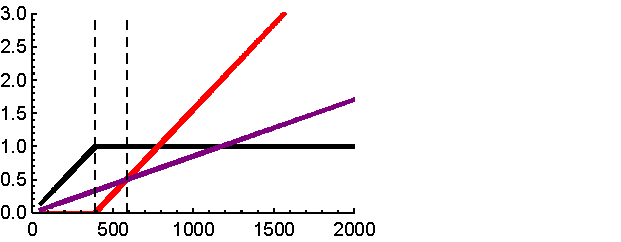
\includegraphics[height=2.5cm]{figures/price1.pdf}}
        \qquad
        \subfloat[A red coin, ETH equivalent to \$1.50, and a portfolio of a red coin and \$0.94.]{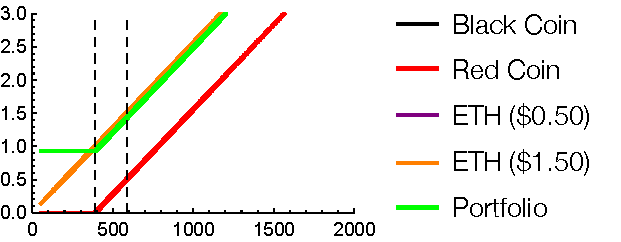
\includegraphics[height=2.5cm]{figures/price2.pdf}}
    \caption[Red-Black Coins Price Changes]{Redemption value in USD (y-axis) as the price of ETH (x-axis) changes. \label{fig:price1} \label{fig:price2}}
\end{figure}

In this section, we answer questions about the financial characteristics of the red-black primitive. Consider a black coin that targets \$1 USD when 1 ETH is \$381.56 USD, and the DApp holds 0.00393126 ETH (worth \$1.5 USD).  Assume for now that (i) a red-black coin is a (non-fungible) contract between two individuals, (ii) it has a fixed maturity date, and (iii) no one intervenes when ETH/USD declines enough that black coins starts to lose value (no liquidations). Figure~\ref{fig:price1}(a) shows how much a black coin is worth (y-axis) as the price of ETH varies (x-axis). The starting point (\$381.56 USD) is marked and if the price of ETH increases (rightward), the black coin is always worth \$1. If the value of ETH decreases (leftward), the black coin is still stable until the value of ETH hits \$254.37 (marked)---at this point, 0.00393126 ETH starts to become worth less than \$1 and the black coin `breaks the buck.'

Figure~\ref{fig:price1}(a) also shows the redemption value of a red coin. When created, a red coin is redeemable for \$0.50 USD. A user with \$0.50 USD can choose between purchasing a red coin or purchasing ETH (also shown). In both cases, the user profits when ETH increases and loses when ETH decreases in price. However the slope of red coin is greater. This indicates it is a \emph{leveraged} position in ETH.  

% = = = = = = = = = = = = = = = = = = = = = = = = = = = = = = = = = = = = = = = = = =

\subsection{How Much Should You Pay for a Black Coin?}

Consider a black coin that is purchased today when ETH is \$381.56 USD. How much will it be worth in 100 days? In most future worlds, the black coin will be worth \$1. In some future worlds (when ETH is worth less than \$254.37), the black coin will break the buck. But even here, it takes a `haircut' on value as opposed to being worthless (\eg it can be redeemed for, say, \$0.90). 

\begin{figure}[t]
    \centering
        \subfloat[Price of ETH in USD (y-axis) over number of days (x-axis).]{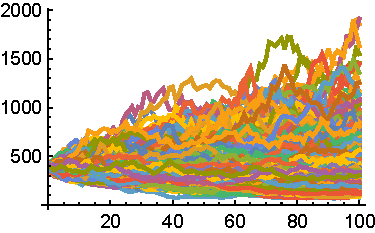
\includegraphics[width=0.4\columnwidth]{figures/mc.pdf}}
        \qquad
        \subfloat[Histogram of final price of ETH in USD (x-axis).]{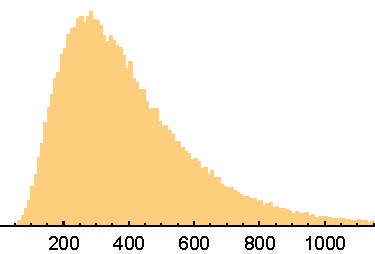
\includegraphics[width=0.4\columnwidth]{figures/histro.pdf}\label{fig:histro}}
    \caption[Monte Carlo Simulation Results]{ETH/USD Monte Carlo simulation results. \label{fig:sim}}
\end{figure}

The average value of a black coin for different possible outcomes can be estimated if we have a statistical model for ETH price movements. In finance, many statistical models have been proposed for many assets. Pricing ETH remains an open research problem. Until future research from the finance community advocates for the most appropriate model, we will sketch in some concrete numbers using Geometric Brownian Motion (GBM), which underlies the Black-Scholes model for pricing options~\cite{BS73} and has been used for ETH in other work~\cite{GPH+20}. We omit the details of the model itself (covered in nearly every  financial textbook~\cite{Sey09}). We fit the model to the historical `closing' prices of ETH for 1000 days prior to 18 Sept 2020\footnote{CoinGecko API: \url{https://api.coingecko.com}} and obtain $\mu=0.000744754$ (an upward drift in price over time) and $\sigma=0.0524172$ (a measure of volatility). If we simulate the next 100 days using Monte Carlo, we obtain the results in Figure~\ref{fig:sim}. For the parameters of this example, the average value of the black coin is \$0.94 USD at the maturity date. Our model can be adjusted for the initial price, over-collateralization ratio (section ~\ref{sec:redchar}), and days until redemption. It is available in Python and Mathematica.\footnote{GitHub: https://github.com/GreatSoshiant/Monte-Carlo/tree/master/Code.} 

As shown in Figure~\ref{fig:sim}\subref{fig:histro}, the expected return is log-normal. When we model more than 100 days, the variance increases and the average redemption value of a black coin decreases: \$0.94 USD after 100 days, \$0.85 USD after 200 days, and \$0.80 after 1 year. This does not mean the black coin is worth less over time, it means the risk it falls out-of-the-money increases the more time you give it. 

% = = = = = = = = = = = = = = = = = = = = = = = = = = = = = = = = = = = = = = = = = =

\subsection{Why Would You Want a Red Coin?}
\label{sec:redchar}

While a stablecoin has utility to the holder, it is less clear what the utility of a red coin is. A red coin is a \textit{leveraged} position in ETH, which means that both gains and losses are amplified---compare the slope of the red coin value with a \$0.50 ETH investment at the same starting point (\$381.56 USD) in Figure~\ref{fig:price1}(a). Leverage is popular with investors. Investing in a red coin is equivalent to investing \$0.50 along with borrowing $2\times\$0.50$ in ETH (\ie 3:1 leverage). If the over-collateralization ratio is decreased from 1.50 to 1.10, then leverage for the red coin increases to 11:1. However, the black coin becomes riskier and its 100-day average value drops from \$0.94 to \$0.86. For a \$2.00 collateralization, red coin leverage is 2:1, and the black coin average value is \$0.98. 

Speculators seek out red coins but what about a user that wants to hold ETH without any leverage? She seemingly has no interest in red (or black) coins. Consider two scenarios: (a) she holds \$1.50 worth of ETH; and (b) she takes her \$1.50 worth of ETH, issues and sells a black coin (\eg for \$0.97 USD), and holds the red coin. She actually has a small portfolio of a red coin and close to \$1 USD. The redemption value of (a) and (b) are depicted in Figure~\ref{fig:price2}(b), along with the red coin by itself. The portfolio is actually an attractive investment---she has `insurance' against catastrophic loss during a devaluation of ETH for a small fixed `fee'---the \$0.03 USD difference between what she received for the black coin (\$0.94) and what the DApp pays out to the black coin holder (\$1.00). Additionally, she produced a stable black coin, which has external benefit to the decentralized economy. 

% = = = = = = = = = = = = = = = = = = = = = = = = = = = = = = = = = = = = = = = = = =

\section{Research Agenda: Extending Red-Black Coins}
\label{sec:taxonomy}

Red-black coins are primitives. Before deploying them, other aspects of their design should to be considered. Design decisions include the maturity/redemption policy, how to make black and red coins fungible, and interventions to prevent the black coin from breaking the buck. One path through the decision tree leads to a design like \dai, however there are many other decisions that could result in very different stablecoins that have not been thoroughly explored by academics or the DeFi community to our knowledge. We do not propose a specific alternative but see our contribution as setting a research agenda. 

%The purpose of this section is to emphasize that \dai is one set of reasonable decisions but there are many alternative designs that have not been (to our knowledge) explored.

% = = = = = = = = = = = = = = = = = = = = = = = = = = = = = = = = = = = = = = = = = =

\subsection{Fungibility}

Assume Alice creates a red/black coin, selling the red coin to Carol. Later, Bob creates a red/black coin, selling the red coin to David. Alice's black coin is not identical to Bob's black coin. Because they were created at different times, the ETH/USD exchange rate is different, and thus the  amount of collateral in ETH in the DApp will be different. The more collateral, the more a black coin is worth (recall Section~\ref{sec:redchar}). Such coins are not interchangeable or \textit{fungible} which adds effort to valuation and exchange. 

One design option is to \textbf{(1) forgo fungibility} and have each coin pair be its own individual contract between two counter-parties (\aka over-the-counter (OTC) contracts). This is the difference between, say, a forward and futures contract~\cite{Har03}. A second option is to \textbf{(2) pool the collateral} of the red coins so that each black coin is a claim against the pool. A pool can be unfair: the losses are democratized to all black coin holders. When pooled, Alice might obtain a black coin before an ETH/USD price bubble; all the black coins issued during the rising bubble are backed by significantly less collateral and when the bubble bursts (consider the case that it reverts to the pre-bubble price), the pool could become under-collateralized, impacting Alice. Had Alice used an OTC contract instead, her red coin would acquire and lose value with the bubble but not be under-collaterialized after bursting. 

A third option is to additionally offer \textbf{(3) red coin fungibility}. Since red coins have variable collateral (based on when they were created), two conditions need to be added to its transfer function: (i) red coins with less than a specified collateral are not transferable, and (ii) red coins with more than the specified collateral will transfer the surplus to the seller’s address while transferring it. While this is not possible with vaults in \dai currently, it seems feasible to add.
	
% = = = = = = = = = = = = = = = = = = = = = = = = = = = = = = = = = = = = = = = = = =

\subsection{Redemption}
\label{sec:maturity}

A policy for redeeming the collateralized ETH is the next design decision. Note that the DApp can autonomously distribute the collateral without the participation of the red or black coin holder, however someone needs to trigger a function call against the DApp to finalize the process.

 Red-black coins could \textbf{(1) mature on a pre-specified date} (\eg the first day of a specified month). At any given time, red/black coins in circulation would have one of a few different expiration dates, while still allowing some degree of fungibility. Coin holders would shorten or extend their coins by trading for a coin with a different maturity date. This is precisely how futures  mature~\cite{Har03}, and yTokens are based on the same principle~\cite{RoNi20}. After maturity, the DApp would lock all transfer functions and only allow withdrawal by the coin holders. The first to ask for a withdrawal would trigger the DApp to look up the ETH/USD price as of the maturity date and split the collateral accordingly. 

Alternatively, red-black coins could be redeemed at any time \textbf{(2) on demand by the black coin holder}, or \textbf{(3) red coin holder}, \textbf{(4) either}, or \textbf{(5) both}. Options (in the US style) work on the principal of (2) or (3)~\cite{Har03,Sey09}. Allowing either to redeem is unlike anything we could find in traditional finance---we speculate it would add uncertainty without any clear gain. Requiring both to agree to redemption could be done by agreement, or (consistent with futures contracts~\cite{Har03}), a red coin holder could acquire a (fungible) black coin and redeem the (netted-out) pair.

% = = = = = = = = = = = = = = = = = = = = = = = = = = = = = = = = = = = = = = = = = = = = = = = = = =

\subsection{Under-collateralization}

When the ETH/USD exchange rate drops enough that under-collateralization is possible, the system could \textbf{(1) do nothing} and let the black coin holder price the risk of this into the coin. If the design attempts further mitigation, the DApp could operate like a margin trading account and require red coin holders to top-up their collateral. If they do not, it is \textbf{(2) liquidated} (\eg sold by auction for black coins). The challenge is incentivizing users to sell USD-pegged black coins for ETH when ETH/USD is in decline (a counter-cyclic investment). In \dai, because collateral is pooled, liquidation is essential because under-collateralized red coins hurt all black coin holders. When collateral is not pooled, liquidation is useless for black coin holders because both ETH and black coins decrease in value at the same rate (recall Figure~\ref{fig:price1}) so it is simpler to do nothing.

Liquidation does not incentivize topped-up collateral unless it is accompanied by a \textbf{(3) punishment} (otherwise red coin holders might try to buy their liquidated assets from themselves at a discount). Beyond charging a fee, a stablecoin system might also withhold rewards (some systems used a secondary token for providing governance and providing rewards) or block red coin transfers until collateral is restored. In traditional financial markets, it is also the case that a trader's margin is inadequate to settle their account, they are still legally liable for the difference. A stablecoin accompanied by a \textbf{(4) reputation system} could mandate that red coin holders settle any obligation, however the potential loses for a red coin holder becomes unbound. A different approach is to obtain \textbf{(5) insurance} or financial coverage for the event of a decline in ETH/USD. This could be actual insurance, whether decentralized or from a traditional brokerage, or an offsetting financial investment that hedges the currency exchange risk. %This is similar to Abra. %Insurance or hedging could be done for a pool of red/black coins, or more simply, it could be done on the individual level (a stablecoin would consist of one black coin and an option to sell for \$1 USD).  

The last approach is \textbf{(6) bail out} any losses through sales of a secondary token. This was used recently by Maker for \dai holders when its normal procedures of (2) and (3) were not adequate for dealing with a sharp, unexpected decline in the price of ETH on 12 Mar 2020 (`black Thursday'). While the auction was successful and recollateralized the pool, it cannot be guaranteed that minting new tokens will be adequate for offsetting any incurred debt. This event also exposed the lack of understanding and underestimation of risk by many vault (\ie red coin) holders who faced losses under (3), and raises the question of whether a system should be designed that is more forgiving to red coin holders in turbulent markets.%, especially since their financial position enables the issuance of a stablecoin. 

% = = = = = = = = = = = = = = = = = = = = = = = = = = = = = = = = = = = = = = = = = = = = = = = = = =

\subsection{Autonomy} 

A design based on the red-black coin primitive that is OTC and does not liquidate is entirely autonomous. It can be instantiated in a DApp and operate without human intervention. While black coins are price-stable under most market conditions, traders who are time-sensitive may forgo obtaining a good price in order to trade quickly. This particularly is influential for stablecoins which provide a low-friction avenue in and out of speculative positions on the price of ETH. Since red and black coins are issued in the same proportion, supply/demand imbalances between them could also add volatility to the black coin price. This could potentially be addressed in the design. 

A non-interventionist approach would let the red and black coin price \textbf{(1) float freely}. This avoids adding complexity to the design---in fact, a design goal might be to design a system that traders can easily understand and grasp the risk of. This could thwart potential lawsuits, such as a recent class action suit against \dai.\footnote{CoinDesk: \url{https://t.co/iJET1JGJib}} An alternative is to further stabilize prices by \textbf{(2) setting rates and fees} at various points in the system. For example, if black coin holders can redeem at any time, a fee could be charged to the black coin holder and paid to the red coin holder. If redemption requires both a red and black coin, the fee could be collected by the DApp. This principle is used by central banks for targeting interest rates, and is used in Maker to control the spot market for \dai. It is a struggle to set fees in the context of a decentralized and autonomous organization---while allowing decisions to be voted on is a first step, it does not guarantee that token holders are independent, informed, and not unduly influenced by the `expert' recommendations. 

% = = = = = = = = = = = = = = = = = = = = = = = = = = = = = = = = = = = = = = = = = = = = = = = = = =
% = = = = = = = = = = = = = = = = = = = = = = = = = = = = = = = = = = = = = = = = = = = = = = = = = =
% = = = = = = = = = = = = = = = = = = = = = = = = = = = = = = = = = = = = = = = = = = = = = = = = = =

\section{Concluding Remarks}

In this chapter, we distil complex stablecoin systems into one of their core primitives, the red-black coin and provide a detailed study of its characteristics and possible extensions. It would be useful to have research results on the most suitable financial model for the ETH/USD price rate (\eg drift-diffusion or GARCH) for us to use in work like this chapter. Future work could also examine the benefits of building a \dai alternative, still based on red-black coins but using different design parameters. Two examples that seem interesting are: (a) a more understandable system that reduces the amount of intervention, and (b) a system with fungible red coins that can be traded freely. Finally, while our research answers the question of how much you should pay for a black coin, the analysis is much more complicated for \dai---with pooled collateral, liquidation, and bailouts, \dai is less risky than a simple black coin but the risk that these countermeasures systemically fail is not zero.



%%%%%%%%%%%%%%%%%%%%%%%%
\chapter{Conclusion and Future Work}
\label{chap:conclusion}

In this thesis, we presented an analysis of three Ethereum components---upgradeability, oracles, and stablecoins---which all add a degree of centrality. They each add trust points to an otherwise decentralized system, increasing the attack surface.

The main takeaways from measuring upgradeability on Ethereum (Chapter 3) is that immutability, as a core property of blockchain, is oversold. Also, we show that almost 64\% of smart contracts are in the control of a centralized agent who can decide to change the whole logic of the system. Future work on upgradability might examine our dataset to learn more about actual upgrade events that have happened on Ethereum. For instance, how many upgrades have happened, how frequently, and what can we determine about the reason behind the upgrade? Undisclosed security vulnerabilities could also be reverse-engineered from an upgrade serving as a security patch. 

The main takeaways from studying oracle systems on Ethereum (Chapter 4) is that most Ethereum projects depend on the data provided by Chainlink, which can be a single point of failure for the Ethereum ecosystem. It highlights a need to diversify which oracle services are used. We also point out that security is reduced to ensuring that the profit from corruption is less than the cost of corruption. Future work should examine how to capture the full extent of the potential profit, considering that attackers may profit outside of Ethereum by attacking oracles on Ethereum. It might conclude this can never be fully captured. 

The main takeways from enumerating the design space of Dai-like stablecoins (Chapter 5) is that they hide risk from the end-user or investor in complex ways that hard to analyze. There is also a prevailing idea that the choices made by MakerDao in designing Dai are the only way to make a stablecoin. We show that there are lots of other suitable designs with differing properties that deserve further research attention. It would also be helpful to have concrete results on the most suitable financial model for the ETH/USD exchange rate (\eg would drift-diffusion or GARCH work better?). Finally, is there a stablecoin design that would be more useful than Dai. Adding fungability to red coins (or CDPs/vaults in Dai) is the most interesting idea from our perspective.

%%%%%%%%%%%%%%%%%%%%%%%%%%%%%%%%%%%%%%%%%%%%%%%%
%% Bibliography
%%%%%%%%%%%%%%%%%%%%%%%%%%%%%%%%%%%%%%%%%%%%%%%%
\clearpage
\phantomsection
\addcontentsline{toc}{chapter}{Bibliography}  %  Add Bibliography to TOC
\singlespacing % save space in the bibliography
\bibliographystyle{abbrv}
\bibliography{references,bib/pulp.bib,bib/new.bib,bib/bib.bib}



%%%%%%%%%% Appendices %%%%%%%%%%%%%%%%
% ---- Appendix settings. Please Do NOT change them. -----
\appendix
\setcounter{table}{0}		% reset the table counter
\setcounter{figure}{0}		% reset the figure counter
\renewcommand{\thefigure}{\Alph{chapter}.\arabic{figure}} 	% numbering the a figure in Appendix as Figure A.2, Figure B.1, etc.
\renewcommand{\thetable}{\Alph{chapter}.\arabic{table}}		% numbering the a table in Appendix as Table A.2, Table B.1, etc.

%%%%%%%%%% Body of Appendix %%%%%%%%%%%%%%%%
%\begin{appendices}
%\doublespacing

%\chapter{First Appendix}
%\label{chap:apdx1}



%\chapter{Concordia Logos}
%\label{chap:logos}
%\begin{figure}[h!]
%	\centering
%	\includegraphics{logos/Concordia_University_logo}
%	\caption{Concordia University}
%\end{figure}
%\vspace{2em}
%\begin{figure}[h!]
%	\centering
%	\includegraphics{logos/Concordia_GinaCody_vertical}
%	\caption{Gina Cody School of Engineering and Computer Science (vertical)}
%\end{figure}
%\vspace{2em}
%\begin{figure}[h!]
%	\centering
%	\includegraphics{logos/Concordia_GinaCody_horizontal}
%	\caption{Gina Cody School of Engineering and Computer Science (horizontal)}
%\end{figure}

%\end{appendices}

\end{document}